\documentclass[fontsize=12pt,paper=a4,twoside,bibtotoc,idxtotoc,
liststotoc,pagesize,BCOR1.2cm,DIV15,chapterprefix,pagesize=pdftex]{scrbook}

%\usepackage[utf8x]{inputenc}
\usepackage[ngerman]{babel}
\usepackage{amsmath}
\usepackage{amssymb}
\usepackage{dsfont}
\usepackage{textcomp}
\usepackage{stmaryrd}
\usepackage{graphicx}
\usepackage{xcolor}
\usepackage{tikz}
\usepackage[xetex,dvipdfmx]{animate}
\usepackage{mathtools}
\usepackage{amsthm}

\theoremstyle{plain}
\newtheorem{sz}[equation]{Satz}
\newtheorem{lm}[equation]{Lemma}
%\newtheorem{pf}{Beweis}
\theoremstyle{definition}
\newtheorem{df}[equation]{Definition}
\newtheorem{nt}[equation]{Notation}
\theoremstyle{remark}
\newtheorem{bem}[equation]{Bemerkung}

\title{Einführung in Sage}
\author{Dr.Jochen Schulz}
\date{10-10-11}


%\usepackage{fontspec,xunicode}
% %\usepackage{polyglossia}
%\setdefaultlanguage[spelling=new, latesthyphen=true]{german}
%\setsansfont{DejaVu Sans}
%\setsansfont{Verdana}
%\setsansfont{Arial}
%\setromanfont[Mapping=tex-text]{Linux Libertine}
%\setsansfont[Mapping=tex-text]{Myriad Pro}
%\setmonofont[Mapping=tex-text]{Courier New}

%\setsansfont{Linux Biolinum}

\usepackage[ngerman]{babel}
\selectlanguage{ngerman}

%
% math/symbols
%
\usepackage{amssymb}
\usepackage{amsthm}
% \usepackage{latexsym}
\usepackage{amsmath}
%\usepackage{amsxtra} %Weitere Extrasymbole
%\usepackage{empheq} %Gleichungen hervorheben
%\usepackage{bm}
 %\bm{A} Boldface im Mathemodus
\usepackage{fontspec,xunicode,xltxtra}

\usepackage{multimedia}
%\usepackage{tikz}

\usepackage{cellspace}
\setlength{\cellspacetoplimit}{2pt}
\setlength{\cellspacebottomlimit}{2pt}

%%%%%%%%%%%%%%%%%% Fuer Frames [fragile]-Option verwenden!
%Programm-Listing
%%%%%%%%%%%%%%%%%%
%Listingsumgebung fuer verbatim
%Grauhinterlegeter Text
%Automatischer Zeilenumbruch ist aktiviert
%\usepackage{listings}
\usepackage[framed]{mcode}
%\usepackage{mcode}
% This command allows you to typeset syntax highlighted Matlab
% code ``inline''.
% mcode fuer matlab

\definecolor{lgray}{gray}{0.80}
\definecolor{gray}{gray}{0.3}
\definecolor{darkgreen}{rgb}{0,0.4,0}
\definecolor{darkblue}{rgb}{0,0,0.8}
\definecolor{key}{rgb}{0,0.5,0} 
\definecolor{NU0}{RGB}{68,85,136} % #458
\definecolor{KW3}{RGB}{85,68,136}
\definecolor{KW4}{RGB}{153,0,0}
\definecolor{dred}{RGB}{221,17,68} % #d14
\definecolor{BG}{RGB}{240,240,240}
%\lstset{backgroundcolor=\color{lgray}, frame=single, basicstyle=\ttfamily, breaklines=true}
%\lstnewenvironment{sage}{\lstset{,language=python, keywordstyle=color{blue},    commentstyle=color{green}, emphstyle=\color{red}, %frame=single, stringstyle=\color{red}, basicstyle=\ttfamily, ,mathescape =true,escapechar=§}}{}

\lstdefinelanguage{fooHaskell} {%
  basicstyle=\footnotesize\ttfamily,%
  commentstyle=\slshape\color{gray},%
  keywordstyle=\bfseries,%\color{KW4},
  breaklines=true,
  sensitive=true,
  xleftmargin=1pc,
  emph={[1]
    FilePath,IOError,abs,acos,acosh,all,and,any,appendFile,approxRational,asTypeOf,asin,
    asinh,atan,atan2,atanh,basicIORun,break,catch,ceiling,chr,compare,concat,concatMap,
    const,cos,cosh,curry,cycle,decodeFloat,denominator,digitToInt,div,divMod,drop,
    dropWhile,either,elem,encodeFloat,enumFrom,enumFromThen,enumFromThenTo,enumFromTo,
    error,even,exp,exponent,fail,filter,flip,floatDigits,floatRadix,floatRange,floor,
    fmap,foldl,foldl1,foldr,foldr1,fromDouble,fromEnum,fromInt,fromInteger,fromIntegral,
    fromRational,fst,gcd,getChar,getContents,getLine,head,id,inRange,index,init,intToDigit,
    interact,ioError,isAlpha,isAlphaNum,isAscii,isControl,isDenormalized,isDigit,isHexDigit,
    isIEEE,isInfinite,isLower,isNaN,isNegativeZero,isOctDigit,isPrint,isSpace,isUpper,iterate,
    last,lcm,length,lex,lexDigits,lexLitChar,lines,log,logBase,lookup,map,mapM,mapM_,max,
    maxBound,maximum,maybe,min,minBound,minimum,mod,negate,not,notElem,null,numerator,odd,
    or,ord,otherwise,pi,pred,primExitWith,print,product,properFraction,putChar,putStr,putStrLn,quot,
    quotRem,range,rangeSize,read,readDec,readFile,readFloat,readHex,readIO,readInt,readList,readLitChar,
    readLn,readOct,readParen,readSigned,reads,readsPrec,realToFrac,recip,rem,repeat,replicate,return,
    reverse,round,scaleFloat,scanl,scanl1,scanr,scanr1,seq,sequence,sequence_,show,showChar,showInt,
    showList,showLitChar,showParen,showSigned,showString,shows,showsPrec,significand,signum,sin,
    sinh,snd,span,splitAt,sqrt,subtract,succ,sum,tail,take,takeWhile,tan,tanh,threadToIOResult,toEnum,
    toInt,toInteger,toLower,toRational,toUpper,truncate,uncurry,undefined,unlines,until,unwords,unzip,
    unzip3,userError,words,writeFile,zip,zip3,zipWith,zipWith3,listArray,doParse
  },%
  emphstyle={[1]\color{NU0}},%
  emph={[2]
    Bool,Char,Double,Either,Float,IO,Integer,Int,Maybe,Ordering,Rational,Ratio,ReadS,Show,ShowS,String,
    Word8,InPacket
  },%
  emphstyle={[2]\bfseries\color{KW4}},%
  emph={[3]
    case,class,data,deriving,do,else,if,import,in,infixl,infixr,instance,let,
    module,of,primitive,then,type,where
  },
  emphstyle={[3]\color{darkblue}},
  emph={[4]
    quot,rem,div,mod,elem,notElem,seq
  },
  emphstyle={[4]\color{NU0}\bfseries},
  emph={[5]
    EQ,False,GT,Just,LT,Left,Nothing,Right,True,Show,Eq,Ord,Num
  },
  emphstyle={[5]\color{KW4}\bfseries},
  morestring=[b]",%
  morestring=[b]',%
  stringstyle=\color{darkgreen},%
  showstringspaces=false
}
\lstnewenvironment{hs}
{\lstset{language=fooHaskell,backgroundcolor=\color{BG}}}
{\smallskip}
\newcommand{\ihs}[1]{\lstset{language=fooHaskell,basicstyle=\color[gray]{0.6}}\lstinline|#1|}


\lstdefinelanguage{fooMatlab} {%
backgroundcolor=\color[gray]{0.9},
breaklines=true,
basicstyle=\ttfamily\small,
%otherkeywords={ =},
%keywordstyle=\color{blue},
%stringstyle=\color{darkgreen},
showstringspaces=false,
%emph={for, while, if, elif, else, not, and, or, printf, break, continue, return, end, function},
%emphstyle=\color{blue},
%emph={[2]True, False, None, self, NaN, NULL},
%emphstyle=[2]\color{key},
%emph={[3]from, import, as},
%emphstyle=[3]\color{blue},
%upquote=true,
%morecomment=[s]{"""}{"""},
%commentstyle=\color{gray}\slshape,
%framexleftmargin=1mm, framextopmargin=1mm, 
%title=\tiny matlab,
frame=single,
%mathescape =true,
%escapechar=§
}
\newcommand{\imatlab}[1]{\lstset{language=fooMatlab,basicstyle=\color[gray]{0.6}}\lstinline|#1|}
\lstnewenvironment{matlab}[1][]{\lstset{language=fooMatlab,xleftmargin=0.2cm,frame=none,backgroundcolor=\color{white},basicstyle=\color{darkblue}\ttfamily\small,#1}}{} 
\lstnewenvironment{matlabin}[1][]{\lstset{language=fooMatlab,#1}}{} 
\newcommand{\matinput}[1]{\lstset{language=fooMatlab}\lstinputlisting{#1}}

\lstdefinelanguage{fooPython} {%
language=python,
backgroundcolor=\color[gray]{0.7},
breaklines=true,
basicstyle=\ttfamily\small,
%otherkeywords={ =},
keywordstyle=\color{blue},
stringstyle=\color{darkgreen},
morestring=[b]",%
morestring=[b]',%
showstringspaces=false,
emph={class, pass, in, for, while, if, is, elif, else, not, and, or,
def, print, exec, break, continue, return, import, from, lambda, null},
emphstyle=\color{blue},
emph={[2]True, False, None, self},
emphstyle=[2]\color{key},
emph={[3]from, import, as},
emphstyle=[3]\color{blue},
upquote=true,
morecomment=[s]{"""}{"""},
comment=[l]{\#},
commentstyle=\color{gray},
%framexleftmargin=1mm, framextopmargin=1mm, 
%title=\tiny python,
%caption=python,
frame=single
%frameround=tttt,
%mathescape =true,
%escapechar=§
}

\newcommand{\pyinput}[1]{\lstset{language=fooPython}\lstinputlisting{#1}}
\newcommand{\isage}[1]{{\lstset{language=fooPython,basicstyle=\color[gray]{0.3}}\lstinline|#1|}}

\lstnewenvironment{pyout}[1][]{\lstset{language=fooPython,xleftmargin=0.2cm,frame=none,backgroundcolor=\color{white},basicstyle=\color{darkblue}\ttfamily\small,#1}}{}
\lstnewenvironment{pyin}[1][]{\lstset{language=fooPython,#1}}{}
\lstnewenvironment{sageout}[1][]{\lstset{language=fooPython,xleftmargin=0.2cm,frame=none,backgroundcolor=\color{white},basicstyle=\color{darkblue}\ttfamily\small,#1}}{}
\lstnewenvironment{sagein}[1][]{\lstset{language=fooPython,#1}}{}

%\usepackage{caption}
%\DeclareCaptionFont{white}{ \color{white} }
%\DeclareCaptionFormat{listing}{
%  \colorbox[cmyk]{0.43, 0.35, 0.35,0.01 }{
%      \parbox{\textwidth}{\hspace{15pt}#1#2#3}
%        }
%        }
%        \captionsetup[lstlisting]{ format=listing, labelfont=white, textfont=white, singlelinecheck=false, margin=0pt, font={bf,footnotesize} }


\usepackage{mydef}
%\usepackage{cmap} % you can search in the pdf for umlauts and ligatures
\usepackage{colonequals} %corrects the definition-symbols \colonequals (besides others)

\usepackage{ifthen}

%%%%%%%%%%%%%%%%%%%
%Neue Definitionen
%%%%%%%%%%%%%%%%%%%

%Newcommands
\newcommand{\Fun}[1]{\mathcal{#1}}      %Mathcal fuer Funktoren
\newcommand{\field}[1]{\mathbb{#1}}     %Grundkoerper ?? in mathds

\newcommand{\A}{\field{A}}              %Affines A
\newcommand{\Fp}{\field{F}_{\!p}}       %Endlicher Koerper mit p Elementen
\newcommand{\Fq}{\field{F}_{\!q}}       %Endlicher Koerper mit q Elementen
\newcommand{\Ga}{\field{G}_{a}}         %Add Gruppenschema
\newcommand{\K}{\field{K}}              %Generischer Koerper 
\newcommand{\N}{\field{N}}              %Nat Zahlen
\newcommand{\Pj}{\field{P}}             %Projektives P
\newcommand{\R}{\field{R}} 		%Reelle Zahlen
\newcommand{\Q}{\field{Q}}              %Rationale Zahlen  
\newcommand{\Qt}{\field{H}}             %Quaternionen 
\newcommand{\V}{\field{V}}              %Vektorbuendel V
\newcommand{\Z}{\field{Z}}              %Ganze Zahlen
\DeclareMathOperator{\Real}{Re}

\newcommand{\fdg}{\;|\;}                 %fuer die gilt

%Operatoren
\DeclareMathOperator{\Abb}{Abb}
%\usepackage{sagetex}


%
% Aufgaben
%
\parindent0cm % Abs�tze nicht einr�cken 
% Definieren einer neuen Farbe
\definecolor{light-gray}{gray}{.9}

\newcounter{zaehler}     % neuen Z�hler einf�hren
\newenvironment{aufgn}[2][0]
%---- Header
{\begin{samepage}%
%\colorbox{light-gray}{%                         % Box in gray
% \makebox[\textwidth]{%                           % Box in linewidth
%\textbf{Aufgabe \arabic{zaehler} } }\hspace{-\textwidth}\makebox[\textwidth]{\hfill #1 Punkte} }\\[0.05cm]       % Header
\dotfill\\
{\large\textbf{Aufgabe \arabic{zaehler} \ifthenelse{ \equal{#2}{} }{}{: \emph{ #2 } }}\ifthenelse{-1=#1}{(testierbar)}{}\ifthenelse{0=#1 \or -1=#1}{}{\hfill #1 Punkte} }\\[0.4cm]
%{\large\textbf{Exercise \arabic{zaehler}  #2 }\ifthenelse{-1=#1}{(testierbar)}{}\ifthenelse{0=#1 \or -1=#1}{}{\hfill #1 Punkte} }\\[0.4cm]
\begin{minipage}{\textwidth}%
}%
%-----  foot
{\end{minipage}\nopagebreak%\begin{minipage}{1cm} \end{minipage}
%\\ 
%\begin{minipage}{0.1cm} \end{minipage} 
%\hrulefill \begin{minipage}{1cm} \end{minipage}\\[1cm]  
\stepcounter{zaehler}                           % increase counter
\end{samepage}%
\\%
\bigskip%
}


\newenvironment{aufg}[1][0]
%---- Header
{\begin{samepage}%
\refstepcounter{zaehler}% increase counter
%\colorbox{light-gray}{%                         % Box in gray
% \makebox[\textwidth]{%                           % Box in linewidth
%\textbf{Aufgabe \arabic{zaehler} } }\hspace{-\textwidth}\makebox[\textwidth]{\hfill #1 Punkte} }\\[0.05cm]       % Header
\dotfill\\
{\large\textbf{Aufgabe \arabic{zaehler} }\ifthenelse{-1=#1}{(testierbar)}{}\ifthenelse{0=#1 \or -1=#1}{}{\hfill #1 Punkte} }\\[0.4cm]
\begin{minipage}{\textwidth}%
}%
%-----  foot
{\end{minipage}\nopagebreak%\begin{minipage}{1cm} \end{minipage}
%\\ 
%\begin{minipage}{0.1cm} \end{minipage} 
%\hrulefill \begin{minipage}{1cm} \end{minipage}\\[1cm]  
\end{samepage}%
\\%
\bigskip%
}

\begin{document}
\maketitle
\tableofcontents

%%%%%%%%%%%%%%%%%%%%%%%%%%%%%%%%%%%%%%
\chapter{Einleitung}
\section{Was ist Sage?}
%\subsection{Was ist Sage?}
%%%%%%%%%%%%%%%%%%%%%%%%%%%%%%%%%%%%%%

Sage ist ein pythonbasiertes, objektorientiertes Open-source (GPL) Mathematik Software System, dass es seit dem 24. Februar 2005 gibt.
In Sage findet man eine Alternative zu den 4 M's: Magma, Maple, Mathematica, Matlab.
Das (Haupt-)Interface ist der Browser, dennoch besitzt Sage Frontends für viele externe Software.
Zu den Stärken von Sage zählt sicherlich, dass es viele andere CAS und Libraries unter einer einheitlichen Oberfläche vereint 
(so z.B. Maxima, Pari, GAP, R, Magma, ...), sowie durch Python eine sehr mächtige Programmiersprache als Grundlage hat. Desweiteren 
ist der Source Code offen, es gibt ein umfangreiches Hilfesystem sowie viele freie Materialien im Internet.
Wie alles, so hat auch Sage trotz seiner vielen Stärken auch Schwächen, so ist der Befehlsumfang nicht so mächtig, wie der von Maple,Mathematica 
oder Matlab; außerdem fehlt eine standalone Entwicklungsumgebung. Als Alternative zum Webinterface findet sich Cantor.

%%%%%%%%%%%%%%%%%%%%%%%%%%%%%%%%%%%%%%
\subsection{Vorab}
%%%%%%%%%%%%%%%%%%%%%%%%%%%%%%%%%%%%%%

Sage incl. online Testversion und gratis Download sowie einigen anderen Features findet sich unter http://www.sagemath.org/.
Hier ein paar grundlegende Tipps, Tricks und Dinge, die einfach beherzigt werden sollten:
\begin{itemize}
 \item Mehrere Befehle in einer Zeile durch {\color{blue} \verb~;~} trennen. 
 \item Bei Eingaben, die über mehrere Zeilen gehen, kann ein
  Zeilenumbruch durch {\color{blue} \verb~<ENTER>~} erreicht werden.
 \item Das Auswerten eines Blocks erfolgt mit {\color{blue} \verb~<SHIFT>+<ENTER>~}.
 \item Ein neues Eingabefeld erhält man durch klicken auf den blauen, horizontalen Balken
 \item {\color{blue} \isage{_} } refenziert die letzte Ausgabe.
 \item Löschen aller eigenen Variablen und Zurücksetzen auf den Anfangsstatus: {\color{blue} \isage{reset()}}
% Anzeigen aller definierten Variablen: {\color{blue} anames(All)}
% Anzeigen aller selbst definierten Variablen: {\color{blue} anames(All,User)}
 \item Das Feld aktivieren von \emph{Typeset} lässt alle Ausgaben von \LaTeX{} rendern.
% profiler und debugger -> commandline
 \item Html- und/oder \LaTeX-Dokumentation:{\color{blue} \verb~<SHIFT>+<KLICK>~ }auf den blauen Balken
% Publish: Im Notebook kann durch klicken des \alert{Publish}-Reiters das Notebook für alle offen gelegt werden. 
% Unter dem Menupunkt \alert{File} kann man 
 \item {\color{blue} Autocompletion :} mit der {\color{blue} \verb~<TAB>~}-Taste erhält man alle möglichen Funktions- und Variablen-Namen im gegebenen Kontext.\\
  Dies gilt insbesondere auch für Objektfunktionen (\isage{object.function()})
  \item{\color{blue} \isage{<command>?} :} gibt ausführliche Hilfe zu \isage{command} an.
 \item {\color{blue} \isage{help(<command>)} :} öffnet ein Hilfefenster zu \isage{command}.
 \item online Dokumentation:
    \begin{itemize}
    \item Sage: http://www.sagemath.org/doc/index.html
    \item Python: http://docs.python.org/
    \end{itemize}
\end{itemize}  


%%%%%%%%%%%%%%%%%%%%%%%%%%%%%%%%%%%%%%
\section{Überblick}
%%%%%%%%%%%%%%%%%%%%%%%%%%%%%%%%%%%%%%

Als Einstieg und kleine Motivation, wofür man Sage einsetzen kann, wollen wir erst einmal ein paar grundlegende Operationen 
vorstellen:
\begin{itemize}
 \item Deklarieren von Variablen mit \isage{var()}, z.B.{\verb~var('a')~} 
 \item Definieren von Variablen mit {\color{blue}'='}, z.B. {\verb~a=3~} 
 \item Definieren von Funktionen mit{\color{blue} '='}, z.B. {\verb~f(x) = x^2 - 6*x~}
 \item Grenzwertbestimmung: {\color{blue}   \verb~f.limit(x=1, dir='<plus|minus>')~}
 \item Bilden von Ableitungen: {\color{blue} \verb~f.differentiate(x)~}
 \item Lösen von Gleichungen: {\color{blue} \verb~solve( f(x)==0, x)~}
 \item Berechnen numerischer Approximationen: {\color{blue} \verb~float(f(sqrt(3)+ 4))~}
 \item Plotten einer Funktion: {\color{blue} \verb~plot(sin,(0,4))~}
 \item symbolisch Integrieren: {\color{blue} \verb~integrate(f,x)~}
 \item numerisch Integrieren: {\color{blue} \verb~integrate(f,x,a,b)~}
 \item Faktorisieren: {\color{blue} \verb~expand(f)~}
 \item Sortieren: {\color{blue} \verb~f.collect(x)~}
 \item Partialbruchzerlegung: {\color{blue} \verb~f.partial_fraction()~}
 \item vollständiges Vereinfachen: {\color{blue} \verb~f.full_simplify()~}
 \item Vereinfachen mit radicals: {\color{blue} \verb~f.radical_simplify()~}
 \item Matrix eingeben: {\color{blue} \verb~matrix([ [z1s1,z1s2],[z2s1,z2s2] ])~}
 \item Vektor eingeben: {\color{blue} \verb~vector([a,b,c])~}
 \item LGS lösen: {\color{blue} \verb~A\b~}
 \item Matrixoperationen: {\color{blue} \verb~A+B,A-B,A*B~}
 \item Matrix invertieren: {\color{blue} \verb~A^(-1); A.inverse()~}
 \item Substitutieren: {\color{blue} \verb~f.subs(k=2)~}
\end{itemize}
Hiermit stehen uns nun einige Türen offen und wir wollen uns durch ein paar Beispiele der Sagewelt nähern:

%%%%%%%%%%%%%%%%%%%%%%%%%%%%%%%%%%%%%%
\subsection{Kurvendiskussion}
%%%%%%%%%%%%%%%%%%%%%%%%%%%%%%%%%%%%%%

Wir wollen eine handelsübliche Kurvendiskussion führen. Dazu betrachten wir die durch die reelle Zahl $a$ parametrisierte 
Funktionenschar:
\[ 
f: x \quad \mapsto \quad \frac{2x^2-20x+42}{x-1}+a, \quad
a \in \mathbb{R} 
\]
Wie bekommen wir nun diese Aufgabe mittels Sage gelöst? Zuerst sollten wir diese Funktionenschar wohl Sage ``erklären'', 
um weiter mit ihr arbeiten zu können. Dies geschieht, indem wir zuerst die Variable $a$ und anschließend die Funktion selbst 
deklarieren:
\begin{sagein}
var('a')
f(x) = (2*x^2-20*x +42)/(x-1)+a;f
\end{sagein}
\begin{bem} Die Multiplikationszeichen dürfen NICHT weggelassen werden.\end{bem}
Wir erhalten als Antwort
\begin{sage}
  x |--> a + 2*(x^2 - 10*x + 21)/(x - 1)
\end{sage}
\begin{bem} Es findet keine Ausgabe statt, wenn wir in unserer Eingabe ;f weglassen.\end{bem}
Wir möchten nun herausfinden, ob unsere Funktion $f$ Polstellen besitzt; dazu benutzen wir den {\color{blue} \verb limit() }-Befehl:
\begin{sagein}
f.limit(x=1, dir='minus')
\end{sagein}
\begin{sage}
  x |--> -Infinity
\end{sage}
\begin{sagein}
f.limit(x=1, dir='plus') 
\end{sagein}
\begin{sage}
  x |--> +Infinity
\end{sage}
Wir sehen nun, dass unsere Funktion $f$ an der Stelle x=1 einen Pol hat. Wir verfahren weiter mit der Suche nach Nullstellen 
und wenden dafür den {\color{blue} \verb solve() }-Befehl an:
\begin{sagein}
solve(f==0,x)
\end{sagein}
\begin{sage}
[x == -1/4*a - 1/4*sqrt(a^2 - 32*a + 64) + 5, x == -1/4*a + 1/4*sqrt(a^2 - 32*a + 64) + 5]
\end{sage}
Wir haben nun 2 Nullstellen gefunden und stellen uns sogleich die Frage nach der Ableitung von $f$, die wir über den 
{\color{blue} \verb differentiate() }-Befehl erhalten:
\begin{sagein}
f.differentiate(x)
\end{sagein}
\begin{sage} 
x |--> 4*(x - 5)/(x - 1) - 2*(x^2 - 10*x + 21)/(x - 1)^2
\end{sage}
Da unsere Funktion $f$ offenbar eine Ableitung besitzt, interessiert uns, ob und, wenn ja, wo $f$ Extrema besitzt sowie die Antwort 
auf die Frage, ob es sich um Minima oder Maxima handelt:
\begin{sagein}
maxi = solve(f.differentiate(x)==0,x); maxi
\end{sagein}
\begin{sage}
[x == -2*sqrt(3) + 1, x == 2*sqrt(3) + 1]
\end{sage}
\begin{sagein}
float( ((f.diff(x)).diff(x))(maxi[0].rhs()) )
\end{sagein}
\begin{sage}
-1.1547005383792501
\end{sage}
\begin{sagein}
float( ((f.diff(x)).diff(x))(maxi[1].rhs()) )
\end{sagein}
\begin{sage}
1.1547005383792515
\end{sage}
Wir erkennen die Existenz zweier Extremstellen, von denen eine ein Maximum, die andere ein Minimum ist.
\begin{bem} Als ``Speicherplatz'' der Nullstellen von $f'$ besitzt maxi zwei Werte-- diese werden mit maxi[0].rhs() 
bzw maxi[1].rhs() angesprochen.\end{bem}
Ohne den {\color{blue} \verb float() }-Befehl sähe die Ausgabe im ersten Fall so aus:
\begin{sagein}
-1/18*((2*sqrt(3) - 1)^2 + 20*sqrt(3) + 11)*sqrt(3) + 2/3*sqrt(3) + 8/3
\end{sagein}
und wäre somit unbrauchbar, um direkt ein Maximum oder Minimum erkennen zu können.
Zuletzt betrachten wir noch das Verhalten am Rande:
\begin{sagein}
f.limit(x=oo); f.limit(x=-oo)
\end{sagein}
\begin{sage}
x |--> +Infinity
x |--> -Infinity
\end{sage}
\begin{bem} Wir erkennen, in Sage stellt sich $\infty$ dar via oo, $-\infty$ entspricht -oo.
Viel interessanter jedoch ist die Tatsache, dass Sage mit jenen ``Werten'' direkt arbeiten zu können scheint.\end{bem}
Zuletzt wollen wir uns mit der grafischen Darstellung einiger Repräsentanten von f auseinandersetzen. Hierzu wollen wir zuerst 3 
jener Repräsentanten deklarieren und diese anschließend mit dem {\color{blue} \verb plot() }-Befehl visualisieren:
\begin{sagein}
 f0 = f(x, a=0)
 f1 = f(x, a=-20)
 f2 = f(x, a=20);f0,f1,f2
\end{sagein}
\begin{sage}
(2*(x^2 - 10*x + 21)/(x - 1), 2*(x^2 - 10*x + 21)/(x - 1) - 20, 2*(x^2 - 10*x + 21)/(x - 1) + 20)
\end{sage}
\begin{sagein}
p = plot(f0,detect_poles='show',xmin=0, xmax=10,color='red')
p += plot(f1,detect_poles='show',xmin=0, xmax=10,color='green')
p += plot(f2,detect_poles='show',xmin=0, xmax=10,color='blue'); p.show(ymin=-80, ymax=80)
\end{sagein}
Wir erhalten als Grafikausgabe:
\begin{center}
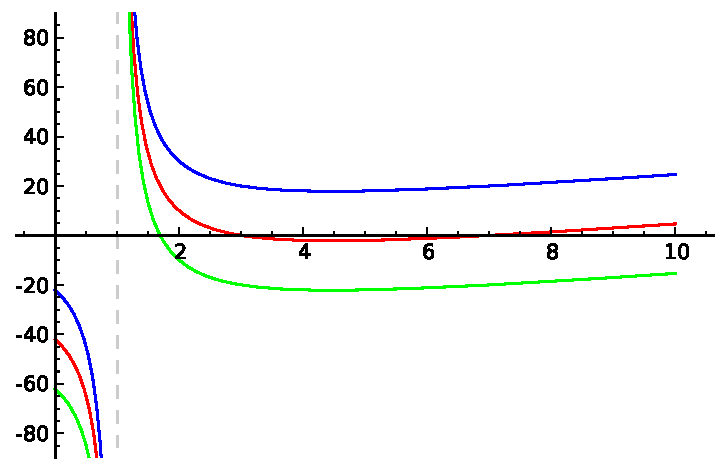
\includegraphics[height=4.5cm]{graphen}
\end{center}

%%%%%%%%%%%%%%%%%%%%%%%%%%%%%%%%%%%%%%
\subsection{Symbolisches Rechnen}
%%%%%%%%%%%%%%%%%%%%%%%%%%%%%%%%%%%%%%

Wir wollen uns nun ein wenig mit symbolischem Rechnen vertraut machen. Dazu zählt das numerische Lösen von Integralen, 
sicherlich aber auch die Vereinfachung oder die Faktorisierung eines Terms. 
Wir betrachten einige Beispiele:
Wir möchten gerne das Integral $\int_0^\infty x^4 e^{-x} dx$ numerisch berechnen, dazu benötigen wir lediglich
\begin{sagein}
integrate(x^4*exp(-x),x,0,oo)
\end{sagein}
und erhalten als Ausgabe 
\begin{sage}
  24
\end{sage}
Wollen wir eine Stammfunktion von $\frac{1+\sin (x)}{1+\cos(x)}$ berechnen, so genügt uns die Deklaration zweier Funktion f
und g wie folgt:
\begin{sagein}
f(x) = (1+sin(x))/(1+cos(x))
g = f.integrate(x);g
\end{sagein}
\begin{sage}
x |--> sin(x)/(cos(x) + 1) - log(cos(x) + 1)
\end{sage}
Die Funktion g sieht eher unschön aus, wir möchten sie daher vereinfachen und benutzen dafür
\begin{sagein}
g.full_simplify()
\end{sagein}
\begin{sage}
x |--> -((cos(x) + 1)*log(cos(x) + 1) - sin(x))/(cos(x) + 1)
\end{sage}
Die Verschönerung hat hier nur bedingt geklappt, aber der Versuch war es wert und oft erhält man wirklich ein schöneres 
Ergebnis als zuvor. Ein wenig effektiver funktioniert es mit ($\frac{e^x -1}{e^{(1/2)x}+1}$)
\begin{sagein}
g = (exp(x)-1)/(exp(x/2)+1)
g.simplify_radical()
\end{sagein}
\begin{sage}
 e^(1/2*x) - 1
\end{sage}
Es gibt noch andere Möglichkeiten, Termen ein schöneres Aussehen zu geben. Betrachten wir den Term
\begin{sage}
x^4 - 10*x^3 + 35*x^2 - 50*x + 24
\end{sage}
und fragen uns: Können wir ihn Faktorisieren? Eine Antwort darauf liefert 
\begin{sagein}
factor(x^4 - 10*x^3 + 35*x^2 - 50*x + 24)
\end{sagein}
\begin{sage}
(x - 4)*(x - 3)*(x - 2)*(x - 1)
\end{sage}
Als kleine Probe können wir die Faktorisierung rückgängig machen:
\begin{sagein}
expand(_)
\end{sagein}
\begin{sage}
x^4 - 10*x^3 + 35*x^2 - 50*x + 24
\end{sage}
\begin{bem} Wir erinnern uns, dass {\color{blue} \verb _ } eine Referenz auf die letzte Ausgabe ist.\end{bem}
Wir können Terme auch bzgl. einer Variablen sortieren:
\begin{sagein}
var('b,a')
g = x^2+2*x+b*x^2+sin(x)+a*x
g.collect(x)
\end{sagein}
\begin{sage}
(b + 1)*x^2 + (a + 2)*x + sin(x)
\end{sage}
Zuletzt steht uns hier noch die Partialbruchzerlegung zur Verfügung:
\begin{sagein}
g = x^ 2/( x^ 2- 1)
g.partial_fraction()
\end{sagein}
\begin{sage}
1/2/(x - 1) - 1/2/(x + 1) + 1
\end{sage}

%%%%%%%%%%%%%%%%%%%%%%%%%%%%%%%%%%%%%%
\subsection{Analytische Geometrie und Lineare Algebra}
%%%%%%%%%%%%%%%%%%%%%%%%%%%%%%%%%%%%%%

Wir wollen uns ein wenig mit analytischer Geometrie und linearer Algebra beschäftigen und zu Anfang mal den Schnittpunkt einer Ebene mit einer Geraden 
berechnen. Dazu sei die Ebene E gegeben durch
\[ E: \vec{x}= 
\left ( \begin{array}{c}  2 \\ 1 \\ -1 \end{array} \right) +l 
\left ( \begin{array}{c}  1 \\ -1 \\ -1 \end{array} \right) +m
\left ( \begin{array}{c}  -3 \\ 1 \\ 4 \end{array} \right), \quad l,m
\in \mathbb{R}
\]
und die Gerade g
\[
g: \vec{x}=
\left ( \begin{array}{c}  3 \\ 0 \\ 1 \end{array} \right) +k
\left ( \begin{array}{c}  4 \\ -1 \\ 2 \end{array} \right), \quad k \in \mathbb{R}
\]
Gleichsetzen ergibt: 
\[ 
\left ( \begin{array}{c}  2 \\ 1 \\ -1 \end{array} \right) +l 
\left ( \begin{array}{c}  1 \\ -1 \\ -1 \end{array} \right) +m
\left ( \begin{array}{c}  -3 \\ 1 \\ 4 \end{array} \right) = \left ( \begin{array}{c}  3 \\ 0 \\ 1 \end{array} \right) +k
\left ( \begin{array}{c}  4 \\ -1 \\ 2 \end{array} \right)
\] oder {
\[ 
\underbrace{\left(   
\begin{array} {ccc} 
1 & -3 & -4\\
-1 & 1 & 1 \\
-1 & 4 & -2  
\end{array} \right)}_{\displaystyle =:A} 
\underbrace{\left ( \begin{array}{c}  l \\ m \\ k \end{array}
  \right)}_{\displaystyle =:L} = \underbrace{\left ( \begin{array}{c}  1 \\ -1 \\ 2
  \end{array} \right)}_{\displaystyle =:b}
\] }
oder $A L=b$.
Wir wollen nun lineare Gleichungssysteme (wie dieses) wie gewöhnlich durch Matrizen beschreiben und via Sage lösen. Dazu benötigen wir ein paar Grundlagen:

 Definieren der Matrix $A$
\begin{sagein}
A = matrix([[1,-3,-4],[-1,1,1],[-1,4,-2]]); A
\end{sagein}
\begin{sage}
[ 1 -3 -4]
[-1  1  1]
[-1  4 -2]
\end{sage}
 Definieren des Vektors $b$
\begin{sagein}
b = vector([1,-1,2]);b
\end{sagein}
\begin{sage}
(1,-1,2) 
\end{sage}
 Lösen von  $A \ L=b$
\begin{sagein}
A.solve_right(b)
\end{sagein}
oder 
\begin{sagein}
A\b
\end{sagein}
ergibt
\begin{sage}
(6/5, 3/5, -2/5)
\end{sage}
 Einsetzen in die Geradengleichung
\begin{sagein}
x_s = matrix([g1,g2,g3]).subs(k=L[2]); x_s
\end{sagein}
\begin{sage}
[7/5 2/5 1/5]
\end{sage}

So haben wir nun recht aufwandsarm den Schnittpunkt der beiden Objekte E und g erhalten. Wir geben noch einen kurzen Ausblick auf weitere 
Matrizenoperationen:
\begin{sagein}
B = matrix([[1,0,0],[0,1,1],[1,1,1]])
A*B, A-B, A+B
\end{sagein}
\begin{sage}
(
[-3 -7 -7]   [ 0 -3 -4]  [ 2 -3 -4]
[ 0  2  2]   [-1  0  0]  [-1  2  2]
[-3  2  2],  [-2  3 -3], [ 0  5 -1]
)
\end{sage}
Berechnen der Inversen (mit Probe)
\begin{sagein}
$A^{(-1)}$, A*A^(-1)
\end{sagein}
\begin{sage}
(
[  -2/5 -22/15   1/15]  [1 0 0]
[  -1/5   -2/5    1/5]  [0 1 0]
[  -1/5  -1/15  -2/15], [0 0 1]
)
\end{sage}
Wir wollen uns das Ganze mal visualisieren, hierzu bietet uns Sage den 3D plot:
\begin{sagein}
var('l,m'); E1 = 2+l-3*m; E2 = 1-l+m; E3 =-1-l+4*m
p = parametric_plot3d([E1,E2,E3],(l,-2,2),(m,-2,2), color='green', opacity=0.8)
var('k'); g1 = 3+4*k; g2 = -k; g3 = 1+2*k
p += parametric_plot3d( (g1,g2,g3), (k, -3, 3),thickness='3' ) 
p.show()
\end{sagein}
\begin{center}
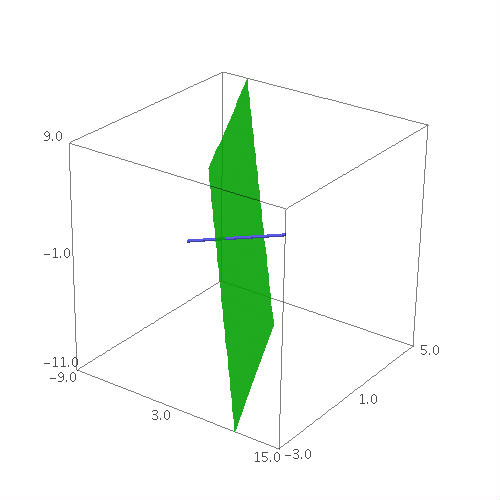
\includegraphics[width=0.7\textwidth]{ebene2}
\end{center}
\begin{bem} In Sage lässt sich der 3D plot drehen.\end{bem}

%%%%%%%%%%%%%%%%%%%%%%%%%%%%%%%%%%%%%%
\subsection{Programmieren}
%%%%%%%%%%%%%%%%%%%%%%%%%%%%%%%%%%%%%%
Sage erlaubt uns, eigene Funktionen von nahezu beliebigem Komplexitätsgrad zu schrieben. Wir wollen uns hier die einzeiligen Funktionen zusammen 
mit Listen und Tupeln sowie Schleifen anschauen-- um im Anschluss etwas Zahlentheorie zu betreiben. Beginnen wir mit den einzeiligen Funktionen, die 
wie folgt aufgebaut sind:
  \begin{sagein}
  def <name>(<Argumente>) : return <Rueckgabe>
  \end{sagein}
Um zu sehen, wie eine solche selbstdefinierte Funktion aussehen könnte, schreiben wir eine Funktion $fd(ex)$, die die Ableitung von $ex$ berechnet 
und sich der Einfachheit halber der sage-internen Funktion {\color{blue} \verb diff() } bedient:
  \begin{sagein}
  def fd(ex) : return diff(ex)
  fd(x^2)
  \end{sagein}
  \begin{sage}
  2*x
  \end{sage}

Sage kennt Listen und Tupel, in denen wir Objekte ablegen, zusammenfassen und noch einiges mehr können. Eine {\color{blue} \verb Liste } 
ist in Sage (und Python) durch \isage{[..,..]}, ein {\color{blue} \verb Tuple } durch \isage{(..,..)} gekennzeichnet. Wir haben einige 
interessante Operationen speziell für Listen:
  \begin{sagein}
  liste = [21,22,24,23]
  liste.sort(); liste 
  \end{sagein}
  \begin{sage}
  [21, 22, 23, 24]
  \end{sage}
\begin{bem}
 Wir erinnern uns, dass durch die {\color{blue} \verb~<TAB>~}-Taste eine Autovervollständigung verfügbar ist. Wenden wir sie auf die Eingabe
{\color{blue} \verb list. } an, erhalten wir eine Auflistung möglicher Operationen auf Listen.
\end{bem}
Fast analog haben wir Tuple:
  \begin{sagein}
  tuple = (liste[0], liste[2])
  tuple, tuple[0]
  \end{sagein}
  \begin{sage}
  ((21, 24), 21) 
  \end{sage}
\begin{bem}
 {\color{blue} \verb liste[i] } liefert das $i$-te Element der Liste liste.
\end{bem}
Wir werden oft eine Liste ganzer Zahlen von \isage{a} bis \isage{b} brauchen, sie von Hand zu erstellen wäre zwar möglich, doch Sage kommt uns 
gern durch sogar 2 Befehle entgegen:
  \begin{sagein}
  [a..b] ; range(a,b+1)
  \end{sagein}
Wir erstellen uns probehalber eine Liste der Zahlen von 1 bis 10:
\begin{sagein}
 a = [1..10];a
\end{sagein}
\begin{sage}
 [1, 2, 3, 4, 5, 6, 7, 8, 9, 10]
\end{sage}
Schauen wir uns nun etwas wirklich nützliches an: Schleifen! Wir unterscheiden grundlegend bedingte und unbedingte Schleifen:
  \begin{sagein}
  [<expr(var)> for <var> in <range|liste>] 
  [<expr(var)> for <var> in <range|liste> if <expr>] 
  \end{sagein}
Als kleine Aufwärmübung wollen wir uns die Quadrate der Zahlen von 1 bis 5 berechnen:
  \begin{sagein}
  [m^2 for m in [1..5] ]
  \end{sagein}
  \begin{sage}
  [1, 4, 9, 16, 25]
  \end{sage}
Und anschließend die Quadrate der Zahlen von 1 bis 5, die durch 2 teilbar sind:
  \begin{sagein}
  [m^2 for m in [1..5] if m%2==0]
  \end{sagein}
  \begin{sage}
  [4, 16]
  \end{sage}

%%%%%%%%%%%%%%%%%%%%%%%%%%%%%%%%%%%%%%
\subsection{Zahlentheorie}
%%%%%%%%%%%%%%%%%%%%%%%%%%%%%%%%%%%%%%

Wir sind nun in der Lage, etwas kompliziertere Aufgabenstellungen zu bearbeiten:
Die Fermatschen Primzahlen sind gegeben durch $F_n=2^{2^n} +1$. Wir wollen die kleinste dieser Zahlen finden, die keine Primzahl ist. Dazu 
schreiben wir uns ein kleines Programm:
\begin{sagein}
def F(n): return 2^(2^n)+1
[[F(m),is_prime(F(m))] for m in range(1,6)]
\end{sagein}
\begin{sage}
[[5, True], [17, True], [257, True], [65537, True], [4294967297, False]]
\end{sage}
Da $F_5$ keine Primzahl ist, interssieren uns nun noch die Teiler von $F_5$
\begin{sagein}
divisors(int(F(5)))
\end{sagein}
\begin{sage}
[1, 641, 6700417, 4294967297]
\end{sage}
 Wir möchten eine Liste der Primzahlen bis 100 und lösen unser Problem durch eine Schleife:
\begin{sagein}
menge = range(1,101)
[m for m in menge if is_prime(m)]
\end{sagein}
\begin{sage}
[2, 3, 5, 7, 11, 13, 17, 19, 23, 29, 31, 37, 41, 43, 47, 53, 59, 61, 67, 71, 73, 79, 83, 89, 97]
\end{sage}
 Sage hätte alternativ die {\color{blue} \verb filter() } Funktion geliefert, die allgemeiner nach (fast) beliebigen Merkmalen filtert:
\begin{sagein}
 filter(is_prime,menge)
\end{sagein}

 Die Mersenne Primzahlen sind gegeben durch $2^p-1$, dabei $p$ Primzahl. Wir wollen die Mersenne Primzahlen im Bereich $\leq200$ bestimmen:
\begin{sagein}
menge = range(1,201)
primes = [m for m in menge if is_prime(m)]
[2^m-1 for m in primes if is_prime(2^m-1)]
\end{sagein}
\begin{sage}
[3, 7, 31, 127, 8191, 131071, 524287, 2147483647, 2305843009213693951,
618970019642690137449562111, 162259276829213363391578010288127,
170141183460469231731687303715884105727]
\end{sage}
Wir widmen uns einer etwas komplizierteren Aufgabe: Wir wollen für die Zahlen $\leq1000$ bestimmen, wieviele Zahlen 1,2,3,... Teiler haben:
\begin{sagein}
menge = range(1,1001)
liste = [number_of_divisors(int(m)) for m in menge]
[(i,len([m for m in liste if m==i]))for i in range(1,51)]
\end{sagein}

\begin{sage}
[(1, 1), (2, 168), (3, 11), (4, 292), (5, 3), (6, 110), (7, 2), (8,
180), (9, 8), (10, 22), (11, 0), (12, 97), (13, 0), (14, 5), (15, 4),
...
\end{sage}
Bis hierher haben wir einen kleinen Rundumblick genommen, einige sehr elementare Grundlagen kennengelernt und sind schon recht vertraut mit 
Sage. Vieles von dem, was wir bisher gesehen haben, wird uns wieder begegnen, wenn wir uns weiter mit Sage befassen.
%%%%%%%%%%%%%%%%%%%%%%%%%%%%%%%%%%%%%%
\chapter{Grundlagen}
\section{Interna}
%%%%%%%%%%%%%%%%%%%%%%%%%%%%%%%%%%%%%%
Um Sage richtig verstehen zu können, ist es wichtig, das ``Innenleben'' zu kennen-- hierzu wollen wir uns anschauen, welche Datentypen Sage 
kennt und wie es mit ihnen umgeht. Hierzu betrachten wir die Funktion $f$
\begin{sagein}
f = x^2-3*x-18
\end{sagein}
und stellen uns einmal folgende Fragen:
\begin{enumerate}
 \item Wie geht Sage mit der Unbekannten $x$ um?
 \item Welchen Datentyp hat $f$?
 \item Was kann ich mit $f$ machen?
\end{enumerate}
Wir wollen die Begriffe Bezeichner, Wert eines Bezeichners, Datentyp und Objekt klar voneinander abgrenzen, hierzu:
\subsubsection{Bezeichner}
\begin{df}
 Bezeichner sind Namen, wie z.B. $x$ oder $f$. Sie können
im mathematischen Kontext sowohl Variablen als auch Unbestimmte repräsentieren.
Bezeichner sind aus Buchstaben, Ziffern und
Unterstrich \_ zusammengesetzt.
Sage unterscheidet zwischen Groß- und Kleinschreibung.
Bezeichner dürfen nicht mit einer Ziffer beginnen.
\end{df}
\begin{bem}
 zulässige Bezeichner:\isage{x}, \isage{f}, \isage{x23}, \isage{_x_1}\\
unzulässige Bezeichner:\isage{12x}, \isage{p~}, \isage{x>y}, \isage{Das System}
\end{bem}
\begin{df}
Der Wert eines Bezeichners  ist ein Objekt eines bestimmten Datentyps.
Ein Datentyp ist durch seine Eigenschaften gegeben.
Ein Objekt ist eine Instanz (Einheit) eines Datentyps.
\end{df}
An dieser Stelle müssen wir uns klarmachen, welche Datentypen Sage kennt-- hierzu eine kleine Übersicht
    \begin{center}
      \begin{tabular}{|lll|}
      \hline
      Typ & Bedeutung & Beispiel\\
      \hline
      \isage{integer} & ganze Zahlen & \isage{-3,0,100}\\
      \isage{rational} & rationale Zahlen & \isage{7/11}\\
      \isage{float} & Gleitpunktzahl & \isage{0.123}\\
      \isage{complex} & komplexe Zahlen & \isage{complex(1,3)}\\
      \isage{expression} & symbolische Ausdrücke & \isage{x+y} \\
      \isage{bool} & logische Werte: true/false& \isage{bool(1<2)} \\
      \hline
      \end{tabular}
    \end{center}
An einigen Beispielen sollten wir uns verdeutlichen, wie Sage diese Datentypen voneinander abgrenzt:
    \begin{sagein}
    type(5)
    \end{sagein}
    \begin{sage}
      <type 'sage.rings.integer.Integer'>
    \end{sage}
    \begin{sagein}
    f = x^2-3*x-18; type(f)
    \end{sagein}
    \begin{sage}
      <type 'sage.symbolic.expression.Expression'>
    \end{sage}
    \begin{sagein}
    type(x)
    \end{sagein}
    \begin{sage}
      <type 'sage.symbolic.expression.Expression'>
    \end{sage}
    \begin{sagein}
    f+f
    \end{sagein}
    \begin{sage}
    2*x^2 - 6*x - 36
    \end{sage}
\subsubsection{Zuweisung}
Nachdem diese Dinge klar sind, betrachten wir Zuweisungen in Sage. Durch {\color{blue} \isage{bez=wert}} wird dem Bezeichner bez der Wert wert
zugewisen. Analoges gilt für Funktionen: Durch {\color{blue} \isage{func(arg)=expr(arg)}} wird die Funktion func mit dem Argument arg definiert, 
die den von arg abhängigen Ausdruck expr auswertet. Da wir einem Bezeichner einen Wert zuweisen können, ist es nur konsequent, das es auch eine 
Methode gibt, die einen Bezeichner von einem Wert befreit: {\color{blue} \isage{reset(bez)}} löscht die Zuweisungen des Bezeichners bez.
\begin{bem}
 Wir beachten, dass durch {\color{blue} \verb = } eine Zuweisung erfolgt, wohingegen {\color{blue} \verb == } der logische Test auf Gleichheit zweier 
Objekte bedeutet.
\end{bem}
Da wir nun das mächtige Werkzeug der Zuweisung beherrschen, welches wir schon die ganze Zeit ``unbewusst'' benutzt haben, wollen wir es auch 
gleich nocheinmal ein wenig ausprobieren:
      \begin{sagein}
      N=6; N
      \end{sagein}
      \begin{sage}
	6
      \end{sage}
      \begin{sagein}
      x,y = var('x,y'); f = x+2*x*x-y; g(x) = x^2; f,g
      \end{sagein}
      \begin{sage}
      (2*x^2 + x - y, x |--> x^2)
      \end{sage}
      \begin{sagein}
      x=pi;y = cos(x); x,y
      \end{sagein}
      \begin{sage}
	(pi, -1)
      \end{sage}
\subsubsection{Auswertung}
Da wir die Zuweisung nun blind beherrschen und auf diese Weise Werte an Bezeichner binden können, stellt sich die Frage nach der Auswertung solcher 
Bezeichner. Dazu halten wir in einer kurzen Definiton folgendes fest:
\begin{df}
 Der Bezeichner ist der Name einer Unbekannten. Die Auswertung eines Bezeichners erfolgt ohne die Benutzung von bekannten Zuweisungen. Der Wert 
bezeichnet die Auswertung zum Zeitpunkt der Zuweisung.
\end{df}
Das wollen wir uns doch genauer ansehen:
    \begin{sagein}
    var('a') ; f(x) = x*x-3*x-a
    \end{sagein}
    \begin{sage}
    x |--> x^2 - a - 3*x
    \end{sage}
    \begin{sagein}
    f(a=2)
    \end{sagein}
    \begin{sage}
    x^2 - 3*x - 2 
    \end{sage}
    \begin{sagein}
    f(1)
    \end{sagein}
    \begin{sage}
      -a - 2
    \end{sage}
    \begin{sagein}
    f(1,a=2)
    \end{sagein}
    \begin{sage}
      -4
    \end{sage}
\subsubsection{Operatoren}
Nun, da wir mit Zuweisung und Auswertung vertraut sind, wollen wir uns den Operatoren und Ausdrücken zuwenden. Auch hierzu eine Begriffsabgrenzung:
\begin{df}
 Operatoren verbinden in Sage Objekte miteinander und sind äquivalent zu Funktionen. Bei der Kombination von Operatoren gelten die üblichen 
Bindungsstärken (also Punktrechnung vor Strichrechnung, Klammerung über alles).
\end{df}
Die in Sage gängigen Operatoren seien hier nur der Vollständigkeit halber aufgeführt:
\begin{center}
\begin{tabular}{|c|l|}
\hline
Operator/Funktion &  Erklärung\\
\hline
\hline
\verb!+! & Addition \\
\verb!-! & Subtraktion\\
\verb!*! & Multiplikation \\
\verb!/! & Division\\
\verb!^! & Potenz\\
\verb!%! &  Rest bei Division\\
\verb!factorial()! & Fakultät \\
\hline
\end{tabular}
\end{center}
\subsubsection{Ausdrücke}
\begin{df}
 In Sage sind Ausdrücke Zusammensetzungen von Operanden ( == Objekte ).
\end{df}
Für Ausdrücke ( == alles ) stehen uns diverse, nennen wir sie einmal ``externe'', Operationen zur Verfügung; so können wir 
beispielsweise die Anzahl ihrer Operanden ({\color{blue} \isage{Ausdruck.nops()}}), ihre Operanden selbst ({\color{blue} \isage{Ausdruck.operands()}}) 
sowie das Vorkommen eines Operanden in einem Ausdruck ermitteln ({\color{blue} \isage{Ausdruck.has(a)}}).
\begin{bem}
 Die Befehle beziehen sich jeweils auf die automatisch vereinfachten Objekte.
\end{bem}
Hierzu wollen wir zwei einfache Beispiele betrachten:
\begin{sagein}
_=var('z,y');f = x*z+3*x+sqrt(y)
f.operands(),(f.operands())[1],((f.operands())[1]).nops()
\end{sagein}
\begin{sage}
([x*z, 3*x, sqrt(y)], 3*x, 2)
\end{sage}
\begin{sagein}
f.has(z), f.has(6) 
\end{sagein}
\begin{sage}
(True, False)
\end{sage}
Da wir sie eben schon kurz angesprochen haben, wollen wir hier einen kurzen, dennoch sehr aufschlussreichen Einschub über die automatische 
Vereinfachung unterbringen:
Sage vereinfacht oft selbstständig. Ist dies einmal nicht der Fall, so haben wir vermöge der Funktion {\color{blue} \verb simplify() } die 
Möglichkeit, eine Vereinfachung anzufordern. Das sieht dann im Prinzip so aus:
\begin{sagein}
sin(15*pi), exp(0)
\end{sagein}
\begin{sage}
(0, 1)
\end{sage}
\begin{sagein}
2*Infinity-5
\end{sagein}
\begin{sage}
+Infinity
\end{sage}
\begin{sagein}
y = (-4*x+x^2+4)*(7*x+x^2+12); y
\end{sagein}
\begin{sage}
(x^2 - 4*x + 4)*(x^2 + 7*x + 12)
\end{sage}
\begin{sagein}
y.full_simplify()
\end{sagein}
\begin{sage}
x^4 + 3*x^3 - 12*x^2 - 20*x + 48
\end{sage}
Da wir uns nun mit der Zuweisung, der Auswertung, Operatoren und Ausdrücken beschäftigt haben, sollte uns interessieren, wie wir unsere 
Ergebnisse, die ja in Sageobjekten stecken, in z.B. einem Text (also in gewisser Art und Weise ``schön'') ausgeben können. Dazu bietet 
Sage die Textausgabe, in der Variablen direkt angesprochen werden können:
\begin{sagein}
print "Text %<format> und %<format> ... " % (x,y,...)}
\end{sagein}
\begin{bem}
 Für \isage{<format>} müssen wir den Datentyp des Objekts einsetzen, also ``i'' für integer oder ``f'' für float, etc. Die Anzahl der 
\isage{<format>}-Platzhalter ist beliebig.
\end{bem}
Wir wollen uns diese Funktionalität an konkreten Beispielen verdeutlichen:
\begin{sagein}
x = 4;y = 6
print "x ist %i und y ist %i" % (x,y)
\end{sagein}
\begin{sage}
x ist 4 und y ist 6
\end{sage}
\begin{sagein}
x = [var("x%i" % k) for k in [1..3]]; x
\end{sagein}
\begin{sage}
[x1, x2, x3]
\end{sage}
Dieses soll uns als Grundlagenwissen über die Sage-interna genügen. Wir werden nun zu anwendungsorientierteren Problemen zurückkehren.
%%%%%%%%%%%%%%%%%%%%%%%%%%%%%%%%%%%%%%
\section{Praxisbezug}
%%%%%%%%%%%%%%%%%%%%%%%%%%%%%%%%%%%%%%
In diesem Abschnitt wollen wir uns mit Funktionen, Code-Blöcken, Bedingungen sowie praktischen Anwendungen befassen.
%%%%%%%%%%%%%%%%%%%%%%%%%%%%%%%%%%%%%%
\subsection{Dictionaries}
%%%%%%%%%%%%%%%%%%%%%%%%%%%%%%%%%%%%%%
Wir wollen ein sageinternes Speichermedium betrachten, das Dictionary. Dabei handelt es sich um ein Konstrukt der Form
\begin{sagein}
d = {<Index1>:<Wert1>,<Index2>:<Wert2>,...}
\end{sagein}
Der Zugriff auf den Inhalt eines solchen Dictionaries geschieht über den Index und liefert, falls vorhanden, den zum Index gehörigen Wert:
\begin{sagein}
d[<Index>]
\end{sagein}
Hier ein kleines Beispiel:
\begin{sagein}
var('x,y,z');d = {x:21,y:5,z:42==y}
d[x],d[z],d[z].rhs()
\end{sagein}
\begin{sage}
(21, 42 == y, y)
\end{sage}
\begin{bem}
 Wir erinnern uns an die Auswirkung der {\color{blue} \verb rhs() }-Funktion. Zugleich erahnen wir, dass Dictionaries, richtig verstanden,
 sehr mächtige Werkzeuge werden können. 
\end{bem}

Wir werden später noch einmal auf dieses nützliche Speichermedium zurückkommen.
%%%%%%%%%%%%%%%%%%%%%%%%%%%%%%%%%%%%%%
\subsection{Funktionen und Abfragen}
%%%%%%%%%%%%%%%%%%%%%%%%%%%%%%%%%%%%%%
Wir betrachten nun Funktionen in Sage. Dazu haben wir zuerst einmal die sog. anonymen Funktionen. Diese sind Funktionen, die keinen aufrufbaren 
Namen besitzen. Sie sind somit ein Funktionen-Objekt. Sinnvoll ist eine anonyme Funktion innerhalb von Konstrukten oder Aufrufen anderer Funktionen.
Eine anonyme Funktion ``lambda'' erstellt man in Sage nach folgendem Schema:
\begin{sagein}
lambda <parameter_list>: <expression> 
\end{sagein}
Wir wollen uns eine anonyme Funktion konstruieren, die die Quadrate der Elemente einer gegebenen Menge berechnet:
\begin{sagein}
menge = [1,2,3,4,5]
map(lambda x: x^2,menge)
\end{sagein}
\begin{sage}
 [1, 4, 9, 16, 25]
\end{sage}
\begin{bem}
 Die Funktion {\color{blue} \verb map() } wendet im Allgemeinen eine Funktion $f$ auf eine gegebene Liste an:
\begin{sagein}
 map(sin, [1, 2, 3])
\end{sagein}
\begin{sage}
 [sin(1), sin(2), sin(3)]
\end{sage}
\end{bem}
\subsubsection{Objektmethoden}
Ein weiterer Funktionentyp sind die sog. Objekt-Methoden, die, wie der Name schon sagt, Funktionen von Objekten sind (wir haben schon einige solcher 
Objekt-Methoden kennengelernt, z.B. die {\color{blue} \verb simplify() }-Funktion). Diese Funktionen werden auf Objekten aufgerufen und sind 
paramterlos (also Objekt.Funktion()). Ein Aufruf der Form Funktion(Objekt) widerspricht der Logik des Programms, wie uns folgender semi-defekter 
Aufruf erhellt:
\begin{sagein}
f = 1 +x -x^2; f.operands(); operands(f)
\end{sagein}
\begin{sage}
[-x^2, x, 1]
Traceback (click to the left of this block for traceback)
...
NameError: name 'operands' is not defined
\end{sage}
\begin{bem}
 f.operands() erzeugt die erste Zeile.
 Den ErrorCode verursacht operands(f).
\end{bem}
Ein Objekt kennt alle auf sich selbst anwendbaren Funktionen; Nur einige Methoden sind als globale Funktionen benutzbar (wie z.B. {\color{blue} \verb map() }).
\subsubsection{Code-Blöcke}
Wir wollen nun unseren Begriff der einzeiligen Schleife auf ganze Code-Blöcke erweitern. Dazu betrachten wir das uns bekannte \verb+[.. for .. in ..]+-Konstrukt. 
Die \verb+for+-Schleife kann von Natur aus ganze Blöcke wiederholen:
\begin{sagein}
for <indexvar> in <expr>/<list>:
    <Code-Block>
else:
    <Code-Block>
\end{sagein}
\begin{bem}
 Wir wollen beachten, dass in Sage (ebenso wie in Python) ein Code-Block durch einen {\color{blue} \verb : } eingeleitet wird und um ein 
{\color{blue} \verb TAB } eingerückt ist.
\end{bem}
Wir machen uns unsere Errungenschaft an einem kleinen Beispiel klar:
\begin{sagein}
x = 2; y = 2
for k in [1..4]:
    x = x +k
    y = y^k
x,y
\end{sagein}
\begin{sage}
(12, 16777216)
\end{sage}
\subsubsection{Abfragen}
Nun, da wir entdeckt haben, dass Sage ganze Code-Blöcke verarbeiten kann, ist es nur konsequent, nach bedingter Ausführung von Code-Blöcken zu verlangen. 
Sage bietet uns hier das {\color{blue} \verb if/else }-Konstrukt:
\begin{sagein}
if <boolean expr>:
    <Code-Block>
\end{sagein}
Auch hierzu benötigen wir ein kleines Beispiel:
\begin{sagein}
x = 3; y = 2
if x > y :
    z = x
else:
    z = y
z
\end{sagein}
\begin{sage}
3
\end{sage}

%%%%%%%%%%%%%%%%%%%%%%%%%%%%%%%%%%%%%%
\subsection{Ausdrücke}
%%%%%%%%%%%%%%%%%%%%%%%%%%%%%%%%%%%%%%
Wir kommen noch einmal zurück zu Ausdrücken, Operationen auf diesen sowie einigen nützlichen Manipulationen. 
\subsubsection{Kombination von Ausdrücken}
Zuerst stellen wir einmal fest, 
dass Ausdrücke nach Belieben miteinander kombiniert werden können. Hierzu definieren wir uns zwei Funktionen $f$ und $g$:
\begin{sagein}
var('x,y'); f = x*x+3*x+y; g = x-y
\end{sagein}
Nun wollen wir, aus einer Laune heraus, f mit g Potenzieren:
\begin{sagein}
f^g
\end{sagein}
\begin{sage}
(x^2 + 3*x + y)^(x - y)
\end{sage}
Offensichtlich kein Problem, auch wenn das Ergebnis recht ``unübersichtlich'' ist (wir erinnern uns an den {\color{blue} \verb simplify() }-Befehl\ldots).
Wie dem auch sei, wenn schon das Potenzieren funktioniert, so werden die übrigen Rechenarten wohl kaum Probleme machen:
\begin{sagein}
f+g, f-g
\end{sagein}
\begin{sage}
(x^2 + 4*x, x^2 + 2*x + 2*y)
\end{sage}
Multiplikation/ Division
\begin{sagein}
f*g, f/g
\end{sagein}
\begin{sage}
((x - y)*(x^2 + 3*x + y), (x^2 + 3*x + y)/(x - y))
\end{sage}
\subsubsection{Vereinfachung von Ausdrücken}
Da wir nun Ausdrücke beliebig kombinieren können, und also auch die Ergebnisse solcher Kombinationen beliebig ``hässlich'' werden können, wollen 
wir uns noch einmal mit verschiedenen Möglichkeiten der ``Verschönerung'' beschäftigen. Dazu stellt Sage uns die Funktionen 
{\color{blue} \verb collect() }, {\color{blue} \verb combine() }, {\color{blue} \verb expand() }, {\color{blue} \verb factor() }, {\color{blue} \verb partial_fraction() } und 
{\color{blue} \verb simplify() } zur Verfügung. Wir betrachten ihre Wirkungsweisen der Reihe nach:
\subsubsection{collect()}
{\color{blue} \isage{a.collect(<unknown>)}} bewirkt, dass der Ausdruck \isage{a} bzgl. der \isage{unknown} Variablen sortiert wird. Das sieht in der Praxis 
dann so aus:
\begin{sagein}
f = a*x^2+a*x+x^3+sin(x)+b*x+4*x+x*sin(x)
f.collect(x)
\end{sagein}
\begin{sage}
a*x^2 + x^3 + (a + b + sin(x) + 4)*x + sin(x)
\end{sage}
\begin{sagein}
f.collect(x*sin(x))
\end{sagein}
\begin{sage}
a*x^2 + x^3 + a*x + b*x + x*sin(x) + 4*x + sin(x)
\end{sage} 
Wir sehen, dass {\color{blue} \verb collect() } bei richtiger Wahl des Arguments eine deutlich wahrnehmbare Übersicht schafft. Sollten wir 
einen Ausdruck vorfinden, der möglicherweise durch Potenzgesetze zu vereinfachen ist, so sollten wir uns an folgenden Befehl erinnern:
\subsubsection{combine()}
{\color{blue} \isage{a.combine()}} bewirkt, dass der Ausdruck durch die Potenzgesetze zusammengefaßt wird.
\begin{sagein}
g = x^(a)*x^(b)
g.combine()
\end{sagein}
\begin{sage}
x^(a + b)
\end{sage}
Wir kennen bereits den {\color{blue} \isage{a.expand()}}-Befehl, den wir hier erweitern wollen.
\subsubsection{expand\_trig()}
Durch {\color{blue} \isage{a.expand_trig()}} wird nach trigonometrischen Eigenschaften ausmultipliziert.
\begin{sagein}
expand((x+2)^4)
\end{sagein}
\begin{sage}
x^4 + 8*x^3 + 24*x^2 + 32*x + 16
\end{sage}
\begin{sagein}
(sin(x+y)).expand_trig()
\end{sagein}
\begin{sage}
sin(x)*cos(y) + sin(y)*cos(x)
\end{sage}
\begin{sagein}
a = (16*x-13)^2 == (3*x+5)^2/2
a.expand()
\end{sagein}
\begin{sage}
256*x^2 - 416*x + 169 == 9/2*x^2 + 15*x + 25/2
\end{sage}
\begin{sagein}
a.expand('left')
\end{sagein}
\begin{sage}
256*x^2 - 416*x + 169 == 1/2*(3*x + 5)^2
\end{sage}
\begin{sagein}
a.expand('right')
\end{sagein}
\begin{sage}
(16*x - 13)^2 == 9/2*x^2 + 15*x + 25/2
\end{sage}
\subsubsection{factor()}
Durch {\color{blue} \isage{factor(Ausdruck)}} wird ein Ausdruck Faktorisiert. 
Sage faktorisiert nur, wenn die resultierenden Koeffizienten rationale 
Zahlen sind. Bei rationalen Funktionen wird ein gemeinsamer Hauptnenner gesucht.
\begin{sagein}
factor(x^2-2), factor(x^2-9/4)
\end{sagein}
\begin{sage}
(x^2 - 2, 1/4*(2*x - 3)*(2*x + 3))
\end{sage}
\begin{sagein}
factor(2 - 2/(x^2-1))
\end{sagein}
\begin{sage}
2*(x^2 - 2)/((x - 1)*(x + 1))
\end{sage}
\subsubsection{f.partial\_fraction()}
Der {\color{blue} \isage{f.partial_fraction()}}-Befehl liefert eine Partialbruchzerlegung.
\begin{sagein}
f = x^2/(x^2-1); f.partial_fraction()
\end{sagein}
\begin{sage}
1/2/(x - 1) - 1/2/(x + 1) + 1
\end{sage}
\begin{sagein}
f = (x^2+2*x+3)/(x^3+4*x^2+5*x+2); f 
\end{sagein}
\begin{sage}
(x^2 + 2*x + 3)/(x^3 + 4*x^2 + 5*x + 2)
\end{sage}
\subsubsection{simplify()}
Hier wollen wir den {\color{blue} \isage{f.simplify()}}-Befehl spezifizieren. {\color{blue} \isage{f.simplify_<target>()}}: vereinfacht den Ausdruck $f$ mit der Methode \isage{<target>}. 
Mögliche targets sind dabei \isage{trig}: trigonometrisch, \isage{rational}: rational, \isage{radical}: log/ln/exp, \isage{factorial}: 
Nutzung der Fakultät, \isage{full}: alle Vereinfachungen. Anwendungen sehen dann zumeist so aus:
\begin{sagein}
(2 - 2/(x^2-1)).simplify_rational()
\end{sagein}
\begin{sage}
2*(x^2 - 2)/(x^2 - 1)
\end{sage}
\begin{sagein}
f = x/(x+y)+y/(x+y)-sin(x)^2-cos(x)^2
f.simplify_rational()
\end{sagein}
\begin{sage}
-sin(x)^2 - cos(x)^2 + 1
\end{sage}
\begin{sagein}
g = sqrt(997)-(997^3)^(1/6)
g.simplify()
\end{sagein}
\begin{sage}
0
\end{sage}
\begin{sagein}
(tan(x)).simplify_trig()
\end{sagein}
\begin{sage}
sin(x)/cos(x)
\end{sage}
\begin{sagein}
a = (2^(1/3)+4^(1/3))^3-6*(2^(1/3) + 4^(1/3))-6
a.simplify_full() 
\end{sagein}
\begin{sage}
0
\end{sage} 
%%%%%%%%%%%%%%%%%%%%%%%%%%%%%%%%%%%%%%
\subsection{Gleichungen, Vergleiche, Logik}
%%%%%%%%%%%%%%%%%%%%%%%%%%%%%%%%%%%%%%
An dieser Stelle wollen wir uns mit Gleichungen, Gleichungssystem und Logik beschäftigen. Dazu betrachten wir zuerst zwei kleine Beispiele 
\begin{sagein}
var('x,y')
Gleichungen = [x+y == 1, x-y == 1]
solve(Gleichungen,x,y)
\end{sagein}
\begin{sage}
[[x == 1, y == 0]]
\end{sage}
\begin{sagein}
Gleichungen1 = [x+y == 1,(x-y)^2 == 1]
solve(Gleichungen1,x,y)
\end{sagein}
\begin{sage}
[[x == 0, y == 1], [x == 1, y == 0]]
\end{sage}
Sage liefert uns offenbar ein sehr gut handhabbares Tool zum Lösen auch komplizierterer Gleichungen, wie das nicht-lineare Beispiel zeigt.
Unsere leichtfertige Benutzung des logischen Operators {\color{blue} \verb == } soll uns hier zum Anlass dienen, Sage einmal genauer auf 
Logik-Tauglichkeit zu untersuchen.
\subsubsection{Logik}
Wir stellen zunächst einmal fest, dass {\color{blue} \verb == } formal den Vergleich zweier Objekte 
auf Gleichheit bedeutet. a==b ist also genau dann wahr, wenn a und b die gleiche Auswertung besitzen und typgleich sind. Mit {\color{blue} \isage{bool(Ausdruck)}} 
haben wir die Möglichkeit, einen Ausdruck auf Wahrheit zu prüfen, logischerweise wird {\color{blue} \verb True } oder {\color{blue} \verb False } 
als Ergebnis zurückgeliefert. Das Gegenteil des {\color{blue} \verb == }-Operators ist der {\color{blue} \verb <> }-Operator-- dementsprechend 
ist a<>b genau dann wahr, wenn a nicht gleich b ist. Wir betrachten zu Verdeutlichung einige Beispiele:
\begin{sagein}
bool(4-3==1)
\end{sagein}
\begin{sage}
True
\end{sage}
\begin{sagein}
bool(4*x==x); x=0; bool(4*x==x)
\end{sagein}
\begin{sage}
False
True
\end{sage}
\begin{sagein}
bool(x==0); bool(x<>0)
\end{sagein}
\begin{sage}
True
False
\end{sage}
\begin{sagein}
bool(0.5==1/2)
\end{sagein}
\begin{sage}
True
\end{sage}
\begin{sagein}
type(0.5); type(1/2)
\end{sagein}
\begin{sage}
<type 'sage.rings.real_mpfr.RealLiteral'>
<type 'sage.rings.rational.Rational'>
\end{sage}
Sage scheint recht gut mit Logik arbeiten zu können-- wir bemerken noch folgendes: Sage kennt das logische 'und' {\color{blue} \verb and }, 
das 'oder' {\color{blue} \verb or } sowie das 'not' {\color{blue} \verb not }. Wiederum der Vollständigkeit halber ein kleines, selbsterklärendes 
Beispiel und die (hoffentlich) bekannte Logiktabelle:
\begin{sagein}
true and false, true or false, not true
\end{sagein}
\begin{sage}
 (False, True, False)
\end{sage}
\begin{center}
\begin{tabular}{|c||c|c|}
\hline
\textbf{and} & \isage{True} & \isage{False}  \\\hline\hline
\isage{True} & \isage{True} & \isage{False}  \\\hline
\isage{False} & \isage{False} & \isage{False} \\\hline
\end{tabular}
\bigskip

\begin{tabular}{|c||c|c|}
\hline
\textbf{or} & \isage{True} & \isage{False} \\\hline\hline
\isage{True} & \isage{True} & \isage{True}  \\\hline
\isage{False} & \isage{True} & \isage{False}  \\\hline
\end{tabular}
\end{center}
\subsubsection{Gleichungssysteme}
Nachdem wir uns nun mit Gleichungen und Logik auseinandergesetzt haben, betrachten wir nun noch Gleichungssysteme. Dabei handelt es sich, aus der 
Sicht von Sage lediglich um eine erweiterung des uns schon wohlbekannten {\color{blue} \verb solve() }-Befehls:
\begin{sagein}
 solve(<gleichungen>,<variablen>,<optionen>)
\end{sagein}
Dabei repräsentiert <gleichungen> das zu lösende System von Gleichungen und <variablen> die Unbekannten der Gleichungen. In <optionen> können 
wir einstellen, ob wir die Lösungen mit Vielfachheiten bekommen möchten ({\color{blue} \verb multiplicities=True }) bzw. ob die Lösungen als Dictionary asugegeben 
werden sollen ({\color{blue} \verb solution_dict=True }). Zu beachten ist, dass bei einzelnen Gleichungen der Lösungswert, bei einem Gleichungssystem 
ein System äquivalenter Gleichungen zurückgeliefert wird. Wir machen uns dies klar an einigen Beispielen.
\begin{sagein}
solve(x^2+x == y/4,x)
\end{sagein}
\begin{sage}
[x == -1/2*sqrt(y + 1) - 1/2, x == 1/2*sqrt(y + 1) - 1/2]
\end{sage}
\begin{sagein}
f = (x-1)^5*(x^2+1)
solve(f == 0, x)
\end{sagein}
\begin{sage}
[x == -I, x == I, x == 1]
\end{sage}
\begin{sagein}
solve(f == 0, x, multiplicities=True)
\end{sagein}
\begin{sage}
([x == -I, x == I, x == 1], [1, 1, 5])
\end{sage}
\begin{sagein}
assume(x>0); solve(x^2+x == y/4,x)
\end{sagein}
\begin{sage}
 [y == 4*x^2 + 4*x]
\end{sage}
\begin{sagein}
solve([x^2-y^2 == 0],[x,y])
\end{sagein}
\begin{sage}
([x == -y, x == y], [1, 1])
\end{sage}
\begin{sagein}
solve([x^2-y^2 == 0, x+y == 1],x,y)
\end{sagein}
\begin{sage}   
[[x == (1/2), y == (1/2)]]
\end{sage}
\begin{sagein}
sol = solve([x^2-y^2 == 0, x+y == 1],x,y, solution_dict=True); sol 
\end{sagein}
\begin{sage}
 [{y: 1/2, x: 1/2}]
\end{sage}
\begin{sagein}
 sol[0][x], sol[0][y]
\end{sagein}
\begin{sage}
 (1/2, 1/2)
\end{sage}
An dieser Stelle betrachten wir noch rasch das numerische Lösen von Gleichungen, hier lediglich im 1-D Fall des Auffindens von Nullstellen 
der Funktion $f$ in einem Intervall $[a,b]$:
\begin{sagein}
f.find_root(a,b) 
\end{sagein}
Exemplarisch sei die Funktion $f(x)=sin(x)$ zu betrachten
\begin{sagein}
 (x == sin(x)).find_root(-2,2)
\end{sagein}
\begin{sage}
0.0
\end{sage}
\begin{bem}
 Der geneigten Leserin wird aufgefallen sein, dass hier tatsächlicherweise nicht die Nullstelle der Funktion $f(x)=sin(x)$ gesucht und gefunden 
wurde, sondern die Suche nach einem Fixpunkt zurückgeführt wurde auf ein Nullstellenproblem. Eine identische Lösung hätte die Nullstellenbetrachtung 
der Funktion $f(x)=sin(x)-x$ geliefert (und tatsächlicherweise auch der Funktion $sin(x)$).
\end{bem}

%%%%%%%%%%%%%%%%%%%%%%%%%%%%%%%%%%%%%%
\chapter{Mengen und Zahlen}
\section{Mengen}
%%%%%%%%%%%%%%%%%%%%%%%%%%%%%%%%%%%%%%
Wie (fast) jedes Kapitel, dass sich mit Mengen auseinandersetzt, so beginnt auch dieses mit der ``gottgegebenen'' Definition des Mengenbegriffs 
nach Cantor:
\begin{quote}
Unter einer Menge verstehen wir jede Zusammenfassung $M$ von bestimmten wohlunterschiedenen Objekten $m$ unserer Anschauung oder unseres Denkens zu einem Ganzen.\\
{\tiny (G. Cantor; Beiträge zur Begründung der transfiniten Mengenlehre; Mathematische Annalen; Bd. 46; 1895; S. 481-512) }
\end{quote}
Die Objekte einer Menge werden Elemente genannt, wir schreiben kurz $x\in M$ für das Element $x$ der Menge $M$. Eine Menge $N$ kann die Menge $M$
enthalten ($M\subset N$) , dies ist der Fall, falls $x\in M \Longrightarrow x\in N$. Wir sprechen von der Gleichheit zweier Mengen $M,N$, falls 
$M\subset N$ und $N\subset M$ gilt.
\subsubsection{Set}
Für Mengen stellt Sage den Typ set bereit. Um eine Menge zu erstellen, benutzen wir die Funktion {\color{blue} \verb Set } und übergeben die Elemente 
direkt mit:
\begin{sagein}
Set([<element1>,<element2>,...])
\end{sagein}
\begin{bem}
 Beachte die doppelte Klammerung.
\end{bem}
Für Sage ist ein set eine ungeordnete Menge von beliebigen Objekten. Der Zugriff auf die Elemente erfolgt, wie üblich, über den Index. Der Aufruf 
{\color{blue} \verb M[n] } würde uns also das $n$-te Elemente der (ungeordneten!) Menge M zurückliefern. Mit {\color{blue} \verb M[i:j] } erhalten wir 
die Elemente mit den Indizes i bis (j-1). Die leere Menge können wir durch {\color{blue} \verb Set([]) } erzeugen. Wir betrachten weitere Beispiele:
\begin{sagein}
M1 = Set([x, 2,3,pi,sqrt(2)]); M1
\end{sagein}
\begin{sage}
{pi, 2, 3, sqrt(2), x}
\end{sage}
\begin{sagein}
var('y');M2 = Set([y,1,Set([1,y]),2,x]); M2
\end{sagein}
\begin{sage}
{1, y, 2, x, {1, y}}
\end{sage}
\begin{sagein}
M2[1]; M2[1:4]
\end{sagein}
\begin{sage}
y
[y, 2, x]
\end{sage}
\subsubsection{Operationen auf Sets}
Wenn Sage mit Mengen richtig umgehen können soll, so müssen elementare Mengenoperationen vorhanden sein. Im Folgenden beschäftigen wir uns mit 
solchen Funktionen:
\subsubsection{cardinality()}
Will man Mengentheorie betrieben, sollte man die ``Größe'' einer Menge wie gewohnt bestimmen können. Hierzu stellt Sage die {\color{blue} \verb cardinality() }- 
Funktion bereit, welche wir auf unsere Menge $M1$ anwenden wollen:
\begin{sagein}
M1.cardinality()
\end{sagein}
\begin{sage}
  5
\end{sage}
% Ändern von Einträgen mit \isage{op} und \isage{subsop} ohne Nebeneffekt:
%\begin{sagein}
%op(M2,3), subsop(M2,3=neu)
%\end{sagein}
%\begin{sage}
%  {1, y}, {1, 2, neu, x, y}
%\end{sage}
\subsubsection{Vereinigung, Differenz, Schnitt}
Weiter sind wir es gewohnt, Mengen schneiden und vereinigen zu können, sowie die Differenz zweier Mengen zu bilden. Hierfür bietet uns Sage die Befehle 
{\color{blue} \verb intersection() }, {\color{blue} \verb union() } und {\color{blue} \verb difference() }. Um uns der Funktionalität gewahr zu werden, betrachten wir folendes 
Minimalbeispiel:
\begin{sagein}
L1 = Set([1,2,3,a,b]); L2 = Set([a,b,c,4,5])
L1.union(L2), L1.difference(L2), L1.intersection(L2)
\end{sagein}
\begin{sage}
({1, 2, 3, 4, a, c, b, 5}, {1, 2, 3}, {b, a})
\end{sage}
Auf die Frage, ob ein Element in einer Menge enthalten ist, liefert folgendes eine aufschlussreiche Antwort:
\begin{sagein}
a in L1, c in L1
\end{sagein}
\begin{sage}
(True, False)
\end{sage}
\begin{sagein}
Set([1,y]) in M2
\end{sagein}
\begin{sage}
True
\end{sage}
\subsubsection{Auswahl nach Eigenschaften}
Betrachten wir etwas ausgefallenere Mengenoperationen. Hierzu erinnern wir uns an die {\color{blue} \verb filter() }-Funktion. Wir wollen 
uns aus einer gegebenen Menge die Primzahlen herausgeben lassen:
\begin{sagein}
M = Set(range(1,15))
filter(is_prime,M)
\end{sagein}
\begin{sage}
  [2, 3, 5, 7, 11, 13]
\end{sage}
Wir wollen die Potenzmenge der Menge $\{1, 2, 3\}$ bestimmen
\begin{sagein}
list(powerset([1,2,3]))
[s for s in Set([1..3]).subsets()]
\end{sagein}
\begin{sage}
[[], [1], [2], [1, 2], [3], [1, 3], [2, 3], [1, 2, 3]]
[{}, {1}, {2}, {3}, {1, 2}, {1, 3}, {2, 3}, {1, 2, 3}]
\end{sage}
\begin{bem}
 Während der erste Befehl eine Liste von Listen erzeugt, erhalten wir im zweiten Fall eine Liste von Mengen. Formal korrekt ist die Potenzmenge 
eine Menge von Mengen.
\end{bem}
\subsubsection{filter()}
Wir wollen uns etwas genauer mit Filtern befassen. Ein Filter erzeugt nach bestimmten Kriterien eine Teilmenge aus einer größeren Menge $M$.
\begin{sagein}
M1 = filter(<f>,<M>)
\end{sagein}
Diese Kriterien sind festgelegt durch die Funktion $f(x)$, die eine Abbildung auf die Boolschen Werte \isage{True/False} ist. 
$M1$ ist die Teilmenge, die aus den Elementen $x\in M$ besteht, für die $f(x)$ eine wahre Aussage ergibt. Wir wollen ein wenig mit Filtern experimentieren:
\begin{sagein}
M = Set(range(1,101))
def f(x): return bool(mod(x,2)==0)
M2 = Set(filter(f,M))
def f(x): return bool(mod(x,15)==0)
M15 = Set(filter(f,M))
M2.intersection(M15)
\end{sagein} 
\begin{sage}
 {90, 60, 30}
\end{sage}
\begin{bem}
 Wir haben hier die durch 2 und 15 teilbaren Elemente der Menge $\{1,\ldots,100\}$ bestimmt.
\end{bem}
Durch eine uns schon bekannte Methode hätten wir den Filter ersetzen können:
\begin{sagein}
M2 = Set([m for m in M if mod(m,2)==0])
M15 = Set([m for m in M if mod(m,15)==0])
M2.intersection(M15)
\end{sagein}
Wir möchten untersuchen, ob eine Menge \isage{A1} eine Teilmenge der Menge \isage{A} ist.
\begin{sagein}
A = Set(range(1,11))
A1 = Set(range(1,3))
A2 = Set(range(9,12))
\end{sagein}
\begin{sagein}
A.intersection(A1) == A1
\end{sagein}
\begin{sage}
  True
\end{sage}
\begin{sagein}
A.intersection(A2) == A2
\end{sagein}
\begin{sage}
  False
\end{sage}
Nachdem wir nun Mengen unser Eigen nennen dürfen, wird es Zeit, dass wir Zahlsysteme, Gruppen und Körper erschließen.
%%%%%%%%%%%%%%%%%%%%%%%%%%%%%%%%%%%%%%
\section{Zahlen}
%%%%%%%%%%%%%%%%%%%%%%%%%%%%%%%%%%%%%%
% andere einfuehrung!
\subsection{Natürliche Zahlen}
Wir wollen noch etwas Zahlentheorie betreiben, die sich dann in lineare Algebra kanalisieren soll. Zunächst führen wir die natürlichen Zahlen nach Peano ein:
\subsubsection{Peano Axiome}
Sei N eine Menge natürlicher Zahlen, für die gilt:
\begin{itemize}
 \item $0 \in N$
 \item Es gibt eien Nachfolgerabbildung $nf:N\rightarrow N\smallsetminus\{0\}$
 \item nf ist injektiv
\end{itemize}
Falls nun gilt, dass $n\in N\Longrightarrow nf(n)\in N \ \forall n\in N$ so ist $N = \mathbb{N}$


Bemerkungen:

 Nachfolgefunktion: $nf(m)=m+1$
 Es besteht ein enger Zusammenhang zwischen den natürlichen
  Zahlen und vollständiger  Induktion.
%TODO:erklaerung  .
 Sage: kein eigener Datentyp (aber: ganze Zahlen (Integer)). 

Sei $M$ eine Menge. Eine {\color{red} Äquivalenzrelation} $R$ auf $M$ ist eine Teilmenge
\[R\subseteq M \times M\]
 mit den folgenden Eigenschaften (Schreibweise: $(x,y) \in R$, $x \sim_R y$, $x \sim y$):

 \textbf{Reflexivität:} für alle $x \in M$ gilt $x \sim x$. 
 \textbf{Symmetrie:} für alle $x,y \in M$ folgt aus $x \sim y$ das $y \sim x$.
 \textbf{Transitivität:} für alle $x,y,z \in M$ und $x \sim y$, $y \sim z$ folgt
  $x \sim z$.  


 Sei $\sim_R$ eine Äquivalenzrelation auf einer Menge $M$.
 Eine Teilmenge $A \subset M$ heißt {\color{red} Äquivalenzklasse}, falls gilt:

 [(a)] $A \neq \emptyset$.
 [(b)] $x,y \in A \ \Rightarrow \ x \sim y$.
 [(c)] $x \in A$, $y \in M$, $x \sim y$ $\Rightarrow$ $y \in A$.

 Eine Äquivalenzrelation zerlegt eine Menge in disjunkte
Äquivalenzklassen.  
 Andersrum definiert eine disjunkte Zerlegung einer Menge eine Äquivalenzrelation.
  Ein $a \in A$ ist ein {\color{red} Repräsentant} der Äquivalenzklasse
$A$. Man schreibt auch $\overline{a}$ oder $a \bmod R$ für ein Äquivalenzklasse $A$. 

Ganze Zahlen: $\mathbb{Z}:=\{ 0,1,-1,2,-2,\dots \}$
% das kann abe rbesser...

 Äquivalenzrelation auf $\mathbb{N} \times \mathbb{N}$:\\
$(m,n) \sim (p,q) \mbox{ genau dann, wenn } m+q=n+p \mbox{ gilt.} $
 Nichtnegative Zahlen: $(m,0)$. Sie sind paarweise nicht äquivalent
zueinander.
 Negative Zahlen: $(0,m)$. 
 Die ganzen Zahlen $\mathbb{Z}$ sind  gegeben durch die Menge
der Äquivalenzklassen.
 Addition:
\[
\overline{(m,n)}+\overline{(u,v)}:=\overline{(m+u,n+v)}\]
 Multiplikation:
\[
\overline{(m,n)}\cdot\overline{(u,v)}:=\overline{(m u+nv,mv+nu)}
\]

Datentyp \isage{Integer}. \\
\textbf{Beispiele:}
\begin{sagein}
type(5), type(0), type(-5)
\end{sagein}
\begin{sage}
(<type 'sage.rings.integer.Integer'>, 
<type 'sage.rings.integer.Integer'>, 
<type 'sage.rings.integer.Integer'>)
\end{sage}
Division
\begin{sagein}
type(5*4), type(5/4)
\end{sagein}
\begin{sage}
(<type 'sage.rings.integer.Integer'>, 
<type 'sage.rings.rational.Rational'>)
\end{sage}
Seien $x \in \mathbb{Z}$, $a \in \mathbb{N}$. Dann gibt es eindeutig bestimmte Zahlen
$n,r \in \mathbb{Z}$ mit $r \in \{0,1,\dots ,a-1\}$, so dass $x=na + r$ gilt. \\
\textbf{Beispiele:}
\begin{sagein}
mod(45,7), floor(45/7)
\end{sagein}
\begin{sage}
(3, 6)
\end{sage}
\begin{sagein}
mod(-34,8), floor(-34/8)
\end{sagein}
\begin{sage}
(6, -5)
\end{sage}
Äquivalenzrelation auf $\mathbb{Z}\times(\mathbb{Z}\smallsetminus \{ 0\})$:
\[ (m,n) \sim (p,q) \mbox{ genau dann, wenn } mq=np \mbox{ gilt.} \]
Statt $(m,n)$ schreibt man $\frac{m}{n}$.

 Die Äquivalenzklasse $\overline{(0,n)}$, $n \in \mathbb{Z}$ ist
die $0$ in $\mathbb{Q}$.
 Mit $(n,m)$ gehören auch alle Erweiterungen $(kn,km)$ zu einer
Ä.-klasse.  
 Addition:  
\[ 
\overline{\genfrac(){}{}{m}{n}}+\overline{\genfrac(){}{}{p}{q}}=\overline{\genfrac(){}{}{mq+pn}{nq}},
\]
Multiplikation:
\[
\overline{\genfrac(){}{}{m}{n}} \ \cdot \ \overline{\genfrac(){}{}{p}{q}}=\overline{\genfrac(){}{}{mp}{nq}}.
\]
% Die rationalen Zahlen bilden einen \alert{Körper}.
 
Datentyp \isage{rational}. 

\begin{sagein}
var('a,b,c,d'); (a/b+c/d).simplify_rational())
\end{sagein}
\begin{sage}
(a*d + b*c)/(b*d)
\end{sage}

\begin{sagein}
bool(a/b+c/d == (a/b+c/d).simplify_rational())
\end{sagein}
\begin{sage}
True
\end{sage}
Eine {\color{red} Gruppe} ist ein Paar $(G,\cdot)$ bestehend aus einer Menge
$G$ und einer Verknüpfung $\cdot$ auf $G$, d.h. einer Abbildung
\[
 \cdot: G \times G \ \rightarrow \ G, \quad (a,b) \mapsto a \cdot b
\]
mit folgenden Eigenschaften

 [(G1)] $(a \cdot b) \cdot c =a \cdot (b \cdot c)$ für alle
$a,b,c \in G$.
 [(G2)] Es existiert ein $e \in G$ ({\it neutrales Element}) mit $e \cdot a =a$ für alle $a
\in G$ und zu jedem $a \in G$ existiert ein $a' \in G$ ({\it inverses
Element}) mit $a' \cdot a=e$. 
  
{\it abelsche} Gruppe: $a \cdot b = b \cdot a$ \emph{für alle} $a,b \in G$.

 Für ein neutrales Element gilt auch $a \cdot e= a$ für alle
$a\in G$.
 Es gibt genau ein neutrales Element $e \in G$.
 Zu jedem $a \in G$ ist das inverse Element $a' \in G$ eindeutig
und wird durch $a^{-1}$ bezeichnet. 
 Es gilt auch $a \cdot a'=e$. 
 Für abelsche Gruppen schreibt man oft $+$ statt $\cdot$. Das Inverse zu $a$ wird dann mit $-a$, das Neutrale mit $0$ bezeichnet.

Ein {\color{red} Körper} ist ein Tripel $(K,+,\cdot)$ bestehend aus einer
Menge $K$ und zwei Verknüpfungen $+$ und $\cdot$ mit folgenden
Eigenschaften:

 [(K1)] $(K,+)$ ist eine abelsche Gruppe. (Das neutrale Element
heiße $0$. Das inverse Element zu $a \in K$ sei $-a$.) 
 [(K2)] $(K \smallsetminus \{ 0 \}, \cdot)$ sei eine abelsche
Gruppe. (Das neutrale Element dazu sei $1$.)
 [(K3)] Distributivgesetze
\begin{eqnarray*}
a \cdot (b + c) & = & (a \cdot b) + (a \cdot c)\\
(a+b) \cdot c & = &   (a \cdot c) + (b \cdot c) \mbox{ für alle }
a,b,c \in K.
\end{eqnarray*}

(Ein Körper ist ein kommutativer unitärer Ring)

BEISPIELE

Gruppen:

 $(\mathbb{Z},+)$, die ganzen Zahlen mit Addition.
 $(\mathbb{Z}/n\mathbb{Z},+)$, die Restklassen modulo $n$ mit Addition.
 $(\mathbb{Q},+)$, $(\mathbb{Q} \smallsetminus \{ 0 \} ,\cdot)$
 $(\mathop{Add}(M,\mathbb{R}),+)$, die reellwertigen Funktionen auf einer Menge $M$ mit punktweiser Addition.
 
Körper:

 Die rationalen Zahlen $\mathbb{Q}$ mit den Verknüpfungen $+$ und $\cdot$.
 Die reellen Zahlen $\mathbb{R}$ mit den Verknüpfungen $+$ und $\cdot$.
 Die komplexen Zahlen $\mathbb{C}$ mit den Verknüpfungen $+$ und $\cdot$.
 Für $p$ Primzahl $\mathbb{Z}/p\mathbb{Z}$, die Restklassen modulo $p$ mit $+$ und $\cdot$.


KÖRPER UND GRUPPEN IN SAGE


 Die ganzen Zahlen  $\mathbb{Z}$: \isage{ZZ}
 Die rationalen Zahlen $\mathbb{Q}$: \isage{QQ} 
 Die reellen Zahlen $\mathbb{R}$: \isage{RR} 
 Die komplexen Zahlen $\mathbb{C}$ : \isage{CC}

\begin{sagein}
QQ(5.01), RR(5/3) 
\end{sagein}
\begin{sage}
(501/100, 1.66666666666667)
\end{sage}
\begin{sagein}
RR.is_field(),ZZ.is_field()
\end{sagein}
\begin{sage}
(True, False)
\end{sage}
Sei $K$ ein Körper. Er heißt {\color{red} angeordnet}, wenn es einen {\color{red}
Positivbereich} $P \subset K$ gibt mit

 Die Mengen $P$, $\{ 0 \}$, und $-P:=\{-x\;|\;x \in P \}$ sind
disjunkt. 
 $K = P \cup \{ 0 \} \cup -P$.
 Aus $x,y \in P$ folgt $x+y \in P$ und $x \cdot y \in P$. 

Man definiert:
\begin{eqnarray*}
 x >y& \text{genau dann, wenn}& x-y\in P,\\
 x \geq y&  \text{genau dann, wenn} &x-y \in P \cup \{ 0 \}.
\end{eqnarray*}
Analog definiert man $<$ und $\leq$. 
Sei $K$ ein angeordneter Körper.

 {\color{red} obere Schranke} $y\in K$: Für $M \subset K$, wenn für alle $x\in M$ die Relation $x \leq y$ gilt.
 nach oben {\color{red} beschränkt}: Wenn eine Teilmenge $M$ von $K$ eine obere Schranke besitzt (analog {\color{red} untere Schranke}).
 {\color{red} Maximum} von $M$: Eine obere Schranke $y$ einer Teilmenge $M \subset K$, wenn $y\in M$ (analog {\color{red} Minimum}).
 {\color{red} Supremum}: Die kleinstmögliche obere Schranke $y$ einer Teilmenge $M \subset K$ (analog {\color{red} Infimum}) 
(Nicht notwendigerweise in $M$ oder $K$).  

REELLE ZAHLEN

 Sei $M$ die Menge aller Teilmengen von $\mathbb{Q}$ mit oberer
Schranke.
 Äquivalenzrelation: Zwei Elemente aus $M$ seien äquivalent, wenn sie dieselben
Mengen von oberen Schranken haben. 
 Die entstehenden Äquivalenzklassen nennt man {\color{red} reelle
Zahlen}.

Bemerkungen

 Es lassen sich die üblichen Verknüpfungen auf $\mathbb{R}$
definieren. 
 Die reellen Zahlen können auch als Vervollständigung von
$\mathbb{Q}$ definiert werden oder durch den Dedekindschen Schnitt.
 Die rationalen Zahlen sind als Äquivalenzklassen der
einelementigen Mengen $\{ x \}$, $x \in \mathbb{Q}$ enthalten.


REELLE ZAHLEN IN SAGE

Datentyp \isage{RealNumber}\\
\textbf{Problem:}
keine exakte Darstellung möglich => Approximation: die Gleitkommazahlen

 Gleitkommazahlen haben in Sage den Datentyp \isage{float}. 
% Gleitkommazahlen werden zur Basis $10$ ausgegeben.
 Die Anzahl der signifikanten Stellen kann durch die Objekt-Methode \isage{n(digits=<digits>)} gesteuert werden
% Intern werden zus\"atzliche Schutzstellen verwendet. Z.B. wird
%bei DIGITS=10 intern mit ca. 19 Stellen gerechnet. ?? nachlesen


\textbf{Beispiel:} $\sqrt{2}$
\begin{sagein}
(sqrt(2)).n(digits=200)
\end{sagein}
\begin{sage}
1.4142135623730950488016887
242096980785696718753769480731767
\end{sage}

FEHLER


 \emph{Relativer Fehler}: Sei $rd(x)$ die 'gerundete' Gleitkomma-Zahl zu $x \in \mathbb{R}$.  Dann gilt
\[ \frac{|x -rd(x)|}{|x|} \leq \varepsilon \]
mit $\varepsilon=b^{1-t}$ ($b$=Basis, $t$=Anzahl signifikante Stellen).
 Rundungsfehler können sich innerhalb eines Verfahrens
verstärken. ({\it Fehlerfortpflanzung}).
 Katastrophale Auswirkungen möglich! Z.B. Absturz der Arianne-Rakete
1996.

Warnung! {\color{red} Die Subtraktion zweier fast gleichgroßer Gleitkommazahlen ist zu
vermeiden.}

NUMERIK


  Berechnen einer numerischen  Näherung
\begin{sagein}
(pi).n(digits=22), (exp(1)).n(digits=22)
\end{sagein}
\begin{sage}
(3.141592653589793238463, 2.718281828459045235360)
\end{sage}
 Sage rechnet mit \isage{floats}, sobald mindestens eine Zahl in
Gleitkommadarstellung gegeben ist 
\begin{sagein}
(1.0+(5/2*3))/(1/7+7/9)^2
\end{sagein}
\begin{sage}
10.0286860879905
\end{sage}
\begin{sagein}
(1+(5/2*3))/(1/7+7/9)^2
\end{sagein}
\begin{sage}
67473/6728
\end{sage}


 Viele Sage Funktionen liefern numerische Werte beim Einsetzen
     von Gleitkommazahlen.
\begin{sagein}
sqrt(64.0), sin(3.14), sin(7/5)
\end{sagein}
\begin{sage}
(8.0000000000000, 0.00159265291648683, sin(7/5))
\end{sage}
 Ausdrücke werden nicht automatisch umgewandelt
\begin{sagein}
2/3*sin(2), 0.666666666666666*sin(2)
\end{sagein}
\begin{sage}
(2/3*sin(2), 0.666666666666666*sin(2))
\end{sage}
\begin{sagein}
float(2/3*sin(2))
\end{sagein}
\begin{sage}
0.60619828455045444
\end{sage}


AUSLÖSCHUNG

\begin{sagein}
x = 10^(-2); ((1.0+x)-1.0)/x
\end{sagein}
\begin{sage}
  1.00000000000000
\end{sage}
\begin{sagein}
x = 10^(-4); ((1.0+x)-1.0)/x
\end{sagein}
\begin{sage}
 0.999999999999890
\end{sage}
\begin{sagein}
x = 10^(-16); ((1.0+x)-1.0)/x
\end{sagein}
\begin{sage}
  0.000000000000000
\end{sage}

\begin{center}
\begin{tabular}{|ll|}
\hline
\isage{abs} & Absolutbetrag\\
\isage{ceil} & Aufrunden\\
\isage{floor} & Abrunden\\
%\isage{frac} & Abschneiden der Vorkommastellen\\
%\isage{trunc} & Abschneiden der Nachkommastellen\\
\isage{round} & Runden\\
%\isage{sign} & Vorzeichen\\
\isage{sqrt} & Wurzel\\
\isage{digits} & Anzahl Stellen\\
%\isage{parent} & Vaterobjekt; Gruppe der Zahl\\
\hline
\end{tabular}
\end{center}


GLEITKOMMAZAHLEN

\[ x=(-1)^{\color{brown} s} \cdot ({\color{red} 0.a_1a_2 \dots a_t}) \cdot {\color{blue}
  b^e}, \quad { \color{red} a_1} \neq 0
\]

 ${\color{blue} b} \in \mathbb{N} \smallsetminus \{ 0, 1\}$ ist die Basis
 ${\color{red} a_1} \neq 0$ erzwingt die Eindeutigkeit der Darstellung.
 ${\color{brown} s \in \{0, 1\}}$ das Vorzeichen.
 Es sei ${\color{red} a_i} \in \{0,1,\dots, b-1 \}$.
 $t$ ist die Anzahl der {\it signifikanten Stellen}.   
 $x$ hat den Wert $(-1)^s b^e \sum_{k=1}^t a_k b^{-k}$. 
 Man spricht von einer {\color{red} $b$-adischen Darstellung} oder einer Darstellung zur Basis $b$.
 
\textbf{Beispiele:}
\[ 73 = {\color{red} 1} \cdot 2^6+{\color{red} 0} \cdot 2^5 +{\color{red} 0} \cdot 2^4 +
  {\color{red} 1} \cdot 2^3 +{\color{red} 0} \cdot 2^2
  + {\color{red} 0} \cdot 2^1 + {\color{red} 1} \cdot 2^0 
\]
$\Rightarrow$ Binärdarstellung {\color{red} $1001001=0.1001001\cdot 2^7$}.
\[
73={\color{blue} 1} \cdot 8^2 + {\color{blue} 1} \cdot 8^1 + {\color{blue} 1} \cdot 8^0
\]
 $\Rightarrow$ Oktaldarstellung {\color{red} $111=0.111 \cdot 8^3$}.
\begin{sagein}
73.str(2)
\end{sagein}
\begin{sage}
1001001
\end{sage}
\begin{sagein}
73.str(8)
\end{sagein}
\begin{sage}
111
\end{sage}
\[ 2.45 = {\color{red} 1} \cdot 2^1 + {\color{red} 0} \cdot 2^0 + {\color{red} 0} \cdot
  2^{-1} + {\color{red} 1} \cdot 2^{-2}+
{\color{red} 1} \cdot 2^{-3} + {\color{red} 1} \cdot 2^{-4}+{\color{red} 0} \cdot 2^{-5}+ \dots \]
$\Rightarrow$ Binärdarstellung {\color{red} \ $10.01110 \dots$}\\

\[ 2.45 = {\color{red} 2} \cdot 8^0 +  {\color{red} 3} \cdot
  8^{-1} + {\color{red} 4} \cdot 8^{-2}+
{\color{red} 6} \cdot 8^{-3} + {\color{red} 3} \cdot 8^{-4}+{\color{red} 1} \cdot 8^{-5}+ \dots \]
$\Rightarrow$ Oktaldarstellung {\color{red} \ $2.34631 \dots$}\\
 \begin{sagein}
 (2.45).str(2)
 \end{sagein}
 \begin{sage}
10.011100110011001100110011001100110011001100110011010
 \end{sage}
 \begin{sagein}
 (2.45).str(8)
 \end{sagein}
 \begin{sage}
2.346314631463146320
 \end{sage}

KOMPLEXE ZAHLEN

Der Körper $\mathbb{C}$ der {\color{red} komplexen Zahlen}:
Die Menge $\mathbb{R}^2=\mathbb{R} \times \mathbb{R}$ mit 

    Addition: $(k,l)+(n,m)=(k+n,l+m)$
 Multiplikation:  $ (k,l) \cdot (n,m) = (kn-lm, km+ln) $



  {\color{red} $i:=(0,1)$}  mit 

 $ i^2=(0,1) \cdot (0,1) = (-1,0) $
 $\forall (x,y) \in \mathbb{C}:  (x,y)=x \cdot (1,0) + y \cdot (0,1)= x +i y$

 \emph{Betrag}: $|z|=|(x,y)|:=\sqrt{x^2+y^2}$ (Sage: \isage{abs})


 \emph{Fundamentalsatz der Algebra}: Jedes nicht konstante Polynom (mit komplexen Koeffizienten) hat mindestens eine Nullstelle in $\mathbb{C}$. 
 Polarkoordinaten $(r, \varphi)$ zu $(x,y) \in \mathbb{C}$
\[  r:= \sqrt{x^2+y^2}, \quad \tan(\varphi)=\frac{y}{x} \] 

 Es gilt: $z = (x,y)_{\text{Rechtwinklig}} = (r,\varphi)_{\text{Polar}} = re^{i\varphi}$


C IN SAGE


 Datentyp in Sage: \isage{complex}
 Die imaginäre Einheit $i=(0,1)$ ist in Sage \isage{I}.
\begin{sagein}
sqrt(-1), I^2
\end{sagein}
\begin{sage}
(I, -1)
\end{sage}
 Rechnen mit komplexen Zahlen
\begin{sagein}
(1+2*I)*(4+I), (1/2+I)*(0.1+I/2)
\end{sagein}
\begin{sage}
 (9*I + 2, -0.4500000000 + 0.3500000000*I)
\end{sage}


  Keine automatische Trennung bzgl. Realteil und  Imaginärteil\\
 \isage{real()}: Realteil
 \isage{imag()}: Imaginärteil
\begin{sagein}
1/(sqrt(2)+I), real(1/(sqrt(2)+I)) + imag(1/(sqrt(2)+I))*I
\end{sagein}
\begin{sage}
1/(sqrt(2) + I)
1/3*sqrt(2) - 1/3*I
\end{sage}
\begin{sagein}
real(1/(sqrt(2)+I)), imag(1/(sqrt(2)+I))
\end{sagein}
\begin{sage}
(1/3*sqrt(2), -1/3)
\end{sage}


%%%%%%%%%%%%%%%%%%%%%%%%%%%%%%%%%%%%%%
\chapter{Vektoren und Funktionen}
\section{Vektoren}
\subsection{Matrizen}
%%%%%%%%%%%%%%%%%%%%%%%%%%%%%%%%%%%%%%

MATRIX

{\color{red} $m \times n$ Matrix} $A=(a_{ij}) \in K^{m\times n}$ über einen Körper $K$ 

\[ A = \left( \begin{array}{cccc}
a_{11} & a_{12} & \cdots & a_{1n} \\
a_{21} & a_{22} & \cdots & a_{2n} \\
\vdots & \vdots & \ddots & \vdots \\
a_{m1} & a_{m2} & \cdots & a_{mn} 
\end{array} \right) \] 
$a_{ij} \in K$, Zeilenindex $i \in [1,m]$, Spaltenindex $j \in [1,n]$

DEFINITIONEN


 {\color{red} Transponiert} von $A=(a_{ij})$: $A^T:=(a_{ji})$ .
 {\color{red} Symmetrisch}: wenn $A=A^T$ gilt.
 \emph{Adjungiert} von $A=(a_{ij})\in \mathbb{C}^{m\times n}$: $A^* :=
(\overline{a_{ji}}) \in \mathbb{C}^{n \times m}$.
 \emph{Einheitsmatrix}: $I:=I_n:=(\delta_{ij}) \in K^{n \times
n}$
 {\color{red} Addition}: Seien $A=(a_{ij}),B=(b_{ij}) \in {K}^{n \times m}$, dann
\[ C=(c_{ij}):=A+B \in {K}^{n \times m} \]
mit $c_{ij}=a_{ij}+b_{ij}$. 
  {\color{red} Multiplikation}: Seien $A=(a_{ij}) \in {K}^{m \times n}$ und $B=(b_{ij})
\in {K}^{n \times p}$, dann 
\[ C=(c_{ij}):=A \cdot B \in{K}^{m \times p} \]
mit $c_{ij}=\sum_{k=1}^n a_{ik} b_{kj}$. 
 {\color{red} orthogonal}: $A \cdot A^T=A^T \cdot A=I_n$ für $A\in K^{n \times n}$ 
 {\color{red} unitär}: $A \cdot A^*=A^* \cdot A=I_n$ für $A\in \mathbb{C}^{n \times n}$.
 {\color{red} invertierbar}: $A\in K^{n \times n}$ heißt , wenn eine
Matrix $A^{-1}\in K^{n \times n}$ existiert mit  $A \cdot
A^{-1}=A^{-1} \cdot A=I_n$.


Bemerkungen


 Die Multiplikation ist assoziativ aber in der Regel \emph{nicht kommutativ}. 
 Die Matrizen aus $K^{m \times n}$ bilden einen Vektorraum über
$K$ (mit komponentenweiser Skalarmultiplikation).
 {\color{red} allgemeine
lineare Gruppe} $\operatorname{GL}(K,n) = \operatorname{GL}_n(K) = \operatorname{GL}(n,K)$: 
Die Menge der invertierbaren Matrizen aus $K^{n \times n}$ bilden bezüglich der Multiplikation eine Gruppe.
 {\color{red} orthogonale Gruppe}: $O(n)$: Die Menge der orthogonalen Matrizen in $GL(\mathbb{R},n)$ bilden
 eine Untergruppe von  $GL(\mathbb{R},n)$. 
  {\color{red} unitäre Gruppe} $U(n)$: Die entsprechende Untergruppe der unitären Matrizen in $GL(\mathbb{C},n)$.


in SAGE

\begin{sagein}
matrix([[a11,a12,...],[a21,a22,..],..])
\end{sagein}


 Der Rückgabewert ist vom Typ \isage{matrix}.
 Die Einträge der Matrix können beliebige Ausdrücke sein.
 Es ist möglich Matrizen über bestimmten Bereichen
(z.B. $\mathbb{R}$, $\mathbb{C}$, $\mathbb{Z}$) zu
konstruieren.                                                     
 Es gibt spezielle Datenstrukturen für quadratische Matrizen und für dünnbesetzte Matrizen. 


KONSTRUKTION

Es gibt in Sage verschiedene Möglichkeiten eine Matrix zu
konstruieren. Beispiel:
\[ A:= \left( \begin{array}{cccc}
1 & 2 & 3 & 4\\
a & 0 & 1 & b\\ 
\end{array} \right), \quad a,b\in \mathbb{R} \]

 Einträge pro Zeile in eckigen Klammern $[ ..]$. Alle
Spalten dann wieder in eckigen Klammern $[ ..]$ (Standard)
\begin{sagein}
A = matrix([[1, 2, 3, 4],[a, 0, 1, b]]) 
\end{sagein}
 Explizite Größenangabe
\begin{sagein}
A = matrix(2,4,[[1,2,3,4],[a,0,1,b]]) 
\end{sagein}
 Nullmatrix der Größe $n \times m$:
\begin{sagein}
n = 3; m = 4; B = matrix(n,m)
\end{sagein}
 Erzeugung mit Hilfe einer Funktion $f(i,j)$ mit Einträgen $a_{ij}=f(i,j)$
\begin{sagein}
f(i,j) = i*j
C = matrix([[f(i,j) for i in range(1,6)] for j in range(1,4)]); C
\end{sagein}
 Eingabe von Zeilen- und Spaltenvektoren (falls explizit nötig)
\begin{sagein}
matrix(3,1,[1,2,3])
matrix(1,3,[4,5,6])
\end{sagein}


ZEILEN/SPALTEN


 Spaltenanzahl: \isage{<matrix>.ncols()}
\begin{sagein}
C.ncols()
\end{sagein}
\begin{sage}
  5
\end{sage}
 Zeilenanzahl: \isage{<matrix>.nrows()}
\begin{sagein}
C.nrows()
\end{sagein}
\begin{sage}
  3
\end{sage}
 Informationen über die Matrix: \isage{<matrix>.parent()}
\begin{sagein}
C.parent()
\end{sagein}
\begin{sage}
Full MatrixSpace of 3 by 5 dense matrices over Symbolic Ring
\end{sage}


ZUGRIFF


 Zugriff auf Einträge in Zeile $i$ und Spalte $j$:
\begin{sagein}
i=1; j=2; C[i,j]
\end{sagein}
\begin{sage}
  6
\end{sage}
 Ändern eines Eintrags in Zeile $i$ und Spalte $j$:
\begin{sagein}
i=1; j=2; C[i,j]=22
\end{sagein}
 Extrahieren von Zeilen/Spalten
\begin{sagein}
zeile = C.row(0)
spalte = C.column(4)
\end{sagein}
 Teilmatrizen
\begin{sagein}
C[1:3,1:3]
\end{sagein}
 Diagonalmatrizen
\begin{sagein}
x = [1,2,3,4,5]
Diag = diagonal_matrix(x); Diag
\end{sagein}


RECHNEN

 
 Addieren, Multiplizieren
\begin{sagein}
var('a,b,c,d,g,h,f')
A = matrix([[a, b], [c,d]])
B = matrix([[e, f], [g,h]])
A+B; A*B
\end{sagein}
 Inverse und der Transponierte
\begin{sagein}
A^(-1); A.transpose()
\end{sagein}


RANG

Sei $A \in K^{m \times n}$. 

 {\color{red} Spaltenrang}: Die Dimension der linearen Hülle der Spaltenvektoren. Er ist höchstens gleich $n$.
 {\color{red} Zeilenrang}: Die Dimension der linearen Hülle der Zeilenvektoren. Er ist höchstens gleich $m$.
 {\color{red} Rang}: Abkürzung, da Zeilenrang und Spaltenrang von Matrizen gleich sind. 


BEISPIELE


 Bestimmen des Ranges einer Matrix
\begin{sagein}
S = matrix([[1,0,0],[0,1,1],[1,1,1]])
S.rank()
\end{sagein}
\begin{sage}
  2
\end{sage}
 ist S symmetrisch ? ist S invertierbar ?
\begin{sagein}
S.is_symmetric() 
S.is_invertible()
\end{sagein}
\begin{sage}
False
False
\end{sage}
 Determinante
\begin{sagein}
S.det()
\end{sagein}
\begin{sage}
  27
\end{sage}

%  Ist eine Matrix unitär ?
% \begin{sagein}
% linalg::isUnitary(S)
% \end{sagein}
% \begin{sage}
%   FALSE
% \end{sage}
% \begin{sagein}
% F:=matrix([[I,0],[0,-I]])
% linalg::isUnitary(F)
% \end{sagein}
% \begin{sage}
%   TRUE
% \end{sage}


MAPS

Anwendung der Funktion \isage{<function>} auf \isage{<matrix>} (siehe auch \isage{map()})\\
\begin{sagein}
map_threaded(<function>,<matrix>)
\end{sagein}
\textbf{Beispiel}:
\begin{sagein}
map_threaded(sqrt,matrix(RR,[[1,2],[3,4]]))
\end{sagein}
  	
\begin{sage}
[1.00000000000000 1.41421356237310]
[1.73205080756888 2.00000000000000] 
\end{sage}

%%%%%%%%%%%%%%%%%%%%%%%%%%%%%%%%%%%%%%
\subsection{Vektorräume}
%%%%%%%%%%%%%%%%%%%%%%%%%%%%%%%%%%%%%%

Ein Tripel $(V,+,\cdot)$, bestehend aus einer nichtleeren Menge $V$
und Verknüpfungen
\[ +:V \times V \ \rightarrow \ V, \qquad \cdot:K\times V \ \rightarrow \ V\]
heißt {\color{red} Vektorraum} über einem Körper
$K$, wenn gilt:

 $(V,+)$ ist eine abelsche Gruppe.
 Für alle $v,w \in V$ und alle $\lambda, \mu \in K$ gilt:

  $(\lambda + \mu) \cdot v  =(\lambda \cdot v) + ( \mu \cdot v)$.
 $\lambda \cdot (v + w )  = ( \lambda \cdot v) + ( \lambda \cdot w)$.
 $(\lambda \mu) \cdot v = \lambda \cdot (\mu \cdot v)$.
 $1 \cdot v = v$.



BEGRIFFE


 {\color{red} Vektoren}: Die Elemente eines Vektorraums.
 {\color{red} Skalarmultiplikation}: Die Abbildung $\cdot : K\times V \ \rightarrow \ V$. Die Elemente des Körpers $K$ nennt man
  {\color{red} Skalare}.
 {\color{red} Untervektorraum} oder {\color{red} Unterraum} von $V$: Ist $U \subset V$ eine Teilmenge des Vektorraums $V$ und es gelten
  alle Vektorraumaxiome.
 \emph{Vorsicht!} man muß zwischen der $0$ des Körpers und der $0$ des Vektorraums (Nullvektor) unterscheiden. \\
Es gilt $0 \cdot v  = 0$ für alle $v \in V$. 


BEISPIELE


 $K^n := \{(x_1,\ldots,x_n) \;|\; x_1, \ldots, x_n \in K\}$, $n \in \mathbb{N}$
 Sei $M$ eine beliebige Menge. Die Menge der Abbildungen von $M$
  in $K$, $\text{Abb}(M,K)$, mit den punktweise definiertenVerknüpfungen
\begin{eqnarray*}
(f+g)(x) & :=& f(x)+g(x), \forall\; x \in M\\
(\alpha \cdot f)(x) & :=& \alpha \cdot f(x), \forall\; x \in M  
\end{eqnarray*}
für $\alpha \in K$, $f,g:M \mapsto K$.
 Die Menge der Polynome bis zum Grad $n$.
 Die Menge aller Polynome.
 $\mathbb{R}$ als $\mathbb{Q}$-Vektorraum.
 $\mathbb{C}$ als $\mathbb{R}$-Vektorraum.


inSAGE

Konstruktion von Vektoren
\begin{sagein}
vector([v1,v2,..]) 
\end{sagein}
\textbf{Beispiele}:

 Konstruktion
\begin{sagein}
a = vector([1,2,3,4]); b = vector([5,6,7]); a,b
\end{sagein}
\begin{small}
\begin{sage}
((1, 2, 3, 4), (5, 6, 7))
\end{sage}
\end{small}
 Datentyp: \isage{vector_integer_dense} (für dichte Vektoren)
\begin{sagein}
type(a)
\end{sagein}
\scriptsize{
\begin{sage}
<type 'sage.modules.vector_integer_dense.Vector_integer_dense'>
\end{sage}}


DEFINITION

Sei $V$ ein $K$-Vektorraum und $(v_1,\dots ,v_r)$ eine Familie von
Elementen aus $V$.

 {\color{red} Linearkombination} $v \in V$ von $(v_1,\dots ,v_r)$: 
  falls $\exists \lambda_1, \dots, \lambda_r \in K$  mit
  $ v= \lambda_1 v_1 + \dots + \lambda_r v_r$. 
 {\color{red} Lineare Hülle} $\mathop{span}\{v_1, \dots, v_n\}$: Die Menge aller Linearkombinationen. Die Lineare
  Hülle ist ein Unterraum von $V$.
 {\color{red} linear unabhängig}: 
  Sind $\lambda_1, \dots , \lambda_r \in K$ und ist $\lambda_1 v_1 +
  \dots + \lambda_r v_r=0$ so folgt $\lambda_1= \dots =
  \lambda_r=0$. Andernfalls {\color{red} linear abhängig}. 

 Ist $M \subseteq V$ eine unendliche Menge, dann ist $M$ linear unabhängig falls alle endlichen Teilmengen von $M$ linear unabhängig sind.



NOTATION

Sei $V$ ein $K$-Vektorraum und $(v_1,\dots ,v_r)$ eine Familie von
Elementen aus $V$

 $(v_1,\dots ,v_r)$ sind genau dann linear unabhängig, wenn sich
jeder Vektor $v \in span\{v_1, \dots ,v_r\}$ eindeutig linear kombinieren
läßt. 
 Vektoren sind linear unabhängig wenn die Determinante der korrelierenden Matrix ungleich 0 ist.
 Gilt $V=span\{v_1,\dots ,v_r \}$, so ist $(v_1, \dots ,v_r)$ ein
{\color{red} Erzeugendensystem}. Sind $(v_1, \dots ,v_r)$ zusätzlich linear
unabhängig, so ist $(v_1, \dots ,v_r)$ eine {\color{red} Basis}.
 Aus jedem Erzeugendensystem kann man eine Basis auswählen. 


BEISPIELE


 Seien $(e_i)_{i=1,\ldots,n} \in \mathbb{R}^n$ die Einheitsvektoren. $(e_1, \dots
,e_n)$ ist eine Basis des $\mathbb{R}^n$.
 Die Monombasis $(1,x,x^2,\dots, x^n)$ ist eine Basis des
Vektorraums der Polynome $n$-ten Grades.
 $(1,i)$ ist eine Basis von $\mathbb{C}$ als
$\mathbb{R}$-Vektorraum. 
 $\mathbb{R}$ als $\mathbb{Q}$-Vektorraum hat keine endliche
Basis. 


BASIS und DIM


 {\color{red} Dimension} des Vektorraums $V$: die  Anzahl der Basiselemente einer Basis $(v_1,\dots, v_n)$.
 Jeder Vektorraum besitzt eine Basis.
 Seien $W,Z$ Unterräume von $V$. Dann ist {\color{red} $W+Z:=span(W \cup Z)$}
die {\color{red} Summe} von $W$ und $Z$. Es gilt:
\[ \dim(W+Z)=\dim(W) + \dim (Z) - \dim( W \cap Z) \]


inSAGE


 Bestimmen einer Basis von $span(s1,s2,s3)$
\begin{sagein}
s1 = vector([1,0,0])
s2 = vector([0,1,1])
s3 = vector([1,1,1])
span([s1,s2,s3],QQ)
\end{sagein}
\begin{sage}
Vector space of degree 3 and dimension 2 over Rational Field
Basis matrix:
[1 0 0]
[0 1 1]
\end{sage}
 Bestimmen des Schnitts von $span(s1)$ und $span(s2,s3)$
\begin{sagein}
span([s1],QQ).intersection(span([s2,s3],QQ))
\end{sagein}
\begin{sage}
Vector space of degree 3 and dimension 1 over Rational Field
Basis matrix:
[1 0 0]
\end{sage}

 Testen der linearen Unabhängigkeit
\begin{sagein}
m = matrix([s1,s2,s3])
m.rank() >= min(m.ncols(), m.nrows())
m.determinant() <> 0 
\end{sagein}

\begin{sage}
  False
\end{sage}


NORMEN

Sei $V$ ein Vektorraum über $K=\mathbb{R}$ oder $K=\mathbb{C}$.\\
Eine {\color{red} Norm} auf $V$ ist eine Abbildung
\[ \| \cdot \|: V \ \rightarrow \mathbb{R}, v \mapsto \| v \|, \]
so dass für  alle $\alpha \in K$, $u,v \in V$ gilt 
\[ \begin{array} {rcl}
\| v \| & \geq & 0 \\
\| v \| & = & 0 \mbox{ impliziert } v=0\\
\| \alpha v \| & = & | \alpha | \| v \|\\
\| u + v \| & \leq & \| u \| + \| v \| \mbox{ (Dreiecksungleichung)}.\\
\end{array} \]
$(V,\| \cdot \|)$
heißt {\color{red} normierter Raum}.

SKALARPROD

Eine skalarwertige binäre Abbildung
\[ ( \cdot, \cdot ): V \times V: \ \rightarrow \ K\]
auf einem Vektorraum $V$ über $K=\mathbb{R}$ oder $K=\mathbb{C}$ heißt
{\color{red} Skalarprodukt}, wenn für alle $x,y,z \in V$, $\alpha, \beta \in
K$ gilt 
\begin{eqnarray*}
(x,x) & \geq & 0\\
(x,x) & = & 0 \mbox{ impliziert } x=0.\\
(x,y) & = & \overline{(y,x)}\\
(\alpha x+\beta y,z) & = & \alpha (x,z)+ \beta (y,z)
\end{eqnarray*}

BEMERKUNG


 Ein VR $V$ mit Skalarprodukt heißt {\color{red} Prä-Hilbert-Raum}. Ist
$K=\mathbb{R}$ so heißt der Raum auch {\color{red} euklidisch}.
 Durch $\|v\|:=\sqrt{(v,v)}$, $v \in V$ läßt sich eine Norm
definieren. Es gilt die {\color{red} Cauchy-Schwarzsche Ungleichung}
\[ |(u,v)| \leq \| u \| \|v\|. \]
 Im euklidischen Raum ist der Winkel $\alpha$ zwischen zwei Vektoren
$u,v \in V\smallsetminus \{ 0 \}$ definiert durch
\[ \cos(\alpha) = \frac{(u,v)}{\|u\| \|v \|}. \]
 {\color{red} Orthogonal}: wenn $(u,v)=0$ gilt.
 {\color{red} Orthogonalbasis}: Eine Basis aus paarweise orthogonalen Vektoren. 
 {\color{red} Orthonormalbasis}: Eine Orthogonalbasis, bei der alle Vektoren die Norm $1$
haben.
 Jeder endlichdimensionale Prä-Hilbert-Raum hat eine
Orthonormalbasis. 
 {\color{red} Orthogonalraum}:
\[
{U}^\perp := \{ v \in V \ | \ (v,u)=0 \mbox{ für alle } u \in U \}
\]
wenn $U$ ein Unterraum von $V$ ist.
 Es gilt: $\dim U + \dim U^\perp = \dim V$, insb. $U \cap U^\perp = 0$.


inSAGE


 $p$-Norm:
\[
\|v\|:=(\sum_{i=1}^n |v_i|^p)^{1/p}, p\in [1,\infty)                   
\]
auf $K^n$ mit $K=\mathbb{R},\mathbb{C}$
\begin{sagein}
x = vector([1,2,3,4,5]); p=2
x.norm(p)
\end{sagein}
 sind Vektoren orthogonal zueinander ?
\begin{sagein}
a1 = vector([1,2,3])
a2 = vector([0,4,1])
a3 = vector([1,1,1])
X = matrix([a1,a2,a3])
X * X.transpose() 
\end{sagein}
 Berechnen des Skalarprodukts
\begin{sagein}
a2.dot_product(a3), a2*a3
\end{sagein}
\begin{sage}
  (5, 5)
\end{sage}
 Berechnen des Winkels zwischen zwei Vektoren
\begin{sagein}
float(acos(a2*a3/(abs(a2)*abs(a3))))
\end{sagein}
\begin{sage}
  0.79520271328967818
\end{sage}


%%%%%%%%%%%%%%%%%%%%%%%%%%%%%%%%%%%%%%
\section{Funktionen}
%%%%%%%%%%%%%%%%%%%%%%%%%%%%%%%%%%%%%%
AUFBAU FKT

\begin{sagein}
def <Name><(a,b,..)>:
    <Code-Block>
    return <ret>
\end{sagein}

 Argumente/Übergabeparameter \isage{(a,b,..)} 
 Jede Zeile, die einen folgenden Block einleitet, muss mit einem Doppelpunkt \isage{:} abgeschlossen werden.
 Jede Zeile in diesem Block muss eine grössere Einrückung besitzen (typischerweise ein \emph{Tab})
 Zeilen gleicher Einrückung gehören zum gleichen Block.
 Rückgabewert \isage{ret} mittels \isage{return(ret)} zurückgegeben. Funktion ist dann beendet.
 Ohne return wird eine leere Variable des Typs \isage{NoneType} zurückgegeben.  


ERKLÄRUNG


 In \isage{\"\"\" comment \"\"\"} eingeschlossene Zeilen werden als Hilfetext abgespeichert und können durch \isage{<funktionsname>?} abgefragt werden.
 Kommentarzeilen: Diese beginnen mit \isage{#}. Sie werden vom System ignoriert.
% Die durch \isage{if <bedingung>:} eingeleitete Zeile ist eine
%  sogenannte Verzweigung. Ist die  Bedingung \isage{<bedingung>} wahr, so wird der
%  Block hinter \isage{:} ausgeführt. Ist \isage{<bedingung>} falsch, so
%  wird die Alternative \isage{else:} ausgeführt.


BEISPIEL

\begin{sagein}
def MyMax(a,b):
    """Maximum von a und b"""
    if a<b:
        return (b)
    else: 
        return (a)
\end{sagein}

 Das Beispiel berechnet das Maximum zweier Zahlen $a$ und
$b$. 
 Aufruf in Sage ist {\color{blue} \isage{MyMax(a,b)}}. 
 Die Funktion gibt dann entweder den Wert $a$ oder den Wert $b$
  zurück.
  

EDIT

Bei umfangreicheren Funktionen oder richtigen Programmen ist es evtl. sinnvoller dies mit
einem Editor zu erstellen. 


  Erstellen einer \verb+<name>.sage+-Datei (Editor: z.B. \verb+geany+)
 \isage{attach <path>/<name>.sage}: hängt die Datei an das Notebook an und wird automatisch geladen und aktuell gehalten.
 \isage{attached_files()}: listet alle angehängte Dateien.


%%%%%%%%%%%%%%%%%%%%%%%%%%%%%%%%%%%%%%
\chapter{Datencontainer, Lineare Abbildungen, Eigenwerte und -vektoren}
\section{Datencontainer in Sage}
\subsection{Folgen}
%%%%%%%%%%%%%%%%%%%%%%%%%%%%%%%%%%%%%%
FOLGEN

\begin{sagein}
 Folge = a,b,c,..
 Folge = tuple(<sequence>)
\end{sagein}


 Ein Tuple ist eine Aneinanderreihung beliebiger Sage-Objekte,
  welche durch Kommata getrennt sind.
 ein Tuple ist in  runde Klammern eingeschlossen.
 Tuple sind ein grundlegender Typ (Listen und Mengen bestehen daraus).

 Einfache Definition
\begin{sagein}
t=var('a,b,c,d,e');Folge1 = a,b,c; Folge2 = (c,d,e); Folge1 ; Folge2
\end{sagein}
\begin{sage}
(a, b, c)
(c, d, e)
\end{sage}
 

KONSTRUKTION


 Mit Listen erzeugte Folgen 
\begin{sagein}
tuple(i^2 for i in range(2,8))
\end{sagein}
\begin{sage}
(4, 9, 16, 25, 36, 49)
\end{sage}

 Erzeugen von $n$ identischen Objekten
\begin{sagein}
tuple(sin(x) for i in range(0,5))
\end{sagein}
\begin{sage}
  (sin(x),sin(x),sin(x),sin(x),sin(x))
\end{sage}
 Erzeugen von $n$ funktionalen Objekten
\begin{sagein}
x = tuple(sin(i) for i in range(1,5)); x
\end{sagein}
\begin{sage}
(sin(1), sin(2), sin(3), sin(4))
\end{sage}  
 Erzeugen einer leeren Folge
\begin{sagein}
folge = (); folge2 = folge,2,3; folge2
\end{sagein}
\begin{sage}
 ((), 2, 3)
\end{sage}



ZUGRIFF


 Verbinden von Folgen
\begin{sagein}
Folge3 = Folge1+Folge2; Folge3
\end{sagein}
\begin{sage}
(a, b, c, c, d, e)
\end{sage}
 Zugriff auf Elemente
\begin{sagein}
x = 1,2,3,4; x[2] 
\end{sagein}
\begin{sage}
  3
\end{sage}
\begin{sagein}
x[2]; x[0:2]
\end{sagein}
\begin{sage}
3
(1, 2)
\end{sage}



%%%%%%%%%%%%%%%%%%%%%%%%%%%%%%%%%%%%%%
\subsection{Listen}
%%%%%%%%%%%%%%%%%%%%%%%%%%%%%%%%%%%%%%
\begin{sagein}
liste = [a,b,c,...] 
liste = list(<sequence>)
\end{sagein}


 Eine Liste ist eine geordnete Folge beliebiger Sage Objekte.
 eine Liste is in eckigen Klammern eingeschlossen.
 Matrizen werden als geschachtelte Listen definiert.
 Baut auf \isage{tuple} auf.
 einfache Konstruktion:
\begin{sagein}
Liste = [1,[1,2], Set([1,2,3]),x]; Liste
\end{sagein}
\begin{sage}
[1, [1, 2], {1, 2, 3}, (1, 2, 3, 4)]
\end{sage}



KONSTRUKTION


 Erzeugen von Listen mit funktionalen Objekten
\begin{sagein}
Liste = [2^i for i in range(1,9)]; Liste
\end{sagein}
\begin{sage}
[2, 4, 8, 16, 32, 64, 128, 256]
\end{sage}
 Leere Listen:
\begin{sagein}
Liste = []; Liste
\end{sagein}
\begin{sage}
  []
\end{sage}


ZUGRIFF


 Der Zugriff funktioniert genau wie bei Folgen.
\begin{sagein}
Liste=[(x,i) for x in range(1,4) for i in range(0,x)];  Liste
\end{sagein}
\begin{sage}
[(1, 0), (2, 0), (2, 1), (3, 0), (3, 1), (3, 2)]
\end{sage}
\begin{sagein}
Liste[3], Liste[5]
\end{sagein}
\begin{sage}
((3, 0), (3, 2))
\end{sage}
 Zuweisung:
\begin{sagein}
Liste[5] = 42; Liste
\end{sagein}
\begin{sage}
  [(1, 0), (2, 0), (2, 1), (3, 0), (3, 1), 42]
\end{sage}


BEFEHLE


 Entfernen eines Elements aus der Liste mit \isage{pop()}
\begin{sagein}
Liste = [a,b,c]; Liste.pop(1); Liste 
\end{sagein}
\begin{sage}
  [a, c]
\end{sage}
 Entfernen eines Elements aus der Liste mit \isage{remove()} 
\begin{sagein}
Liste = [a,b,c]; Liste.remove(b); Liste
\end{sagein}
\begin{sage}
  [a, c]
\end{sage}
 Anhängen eines Elementes mittels \isage{append()}
\begin{sagein}
Liste.append([3,4,5]); Liste
\end{sagein}
\begin{sage}
[a, c, [3, 4, 5]]
\end{sage}
 Zusammenfügen von Listen mit dem $+$- und $*$-Operator. 
\begin{sagein}
Liste2 = Liste+[3,4,5]; Liste2
\end{sagein}
\begin{sage}
[a, c, [3, 4, 5], 3, 4, 5]
\end{sage}
\begin{sagein}
Liste*2
\end{sagein}
\begin{sage}
 [a, c, [3, 4, 5], a, c, [3, 4, 5]]
\end{sage}
 Sortieren von Listen mit \isage{sort()}
\begin{sagein}
Liste = [4,-23,1,3]; Liste.sort(cmp=lambda x,y: int(2*(abs(x)>abs(y))-1)); Liste
\end{sagein}
\begin{sage}
[1, 3, 4, -23]
\end{sage}


INKLUSIONEN


  Ist Objekt \isage{Objekt} in der Liste \isage{Liste} enthalten?
\begin{sagein}
 <Objekt> in <Liste>
\end{sagein}
Beispiel:
\begin{sagein}
Liste = [x+1,a,x+1,sin(b)]
x+1 in Liste
\end{sagein}
\begin{sage}
  True
\end{sage}
 Position des Objektes in der Liste (bei Fehlen gibt es eine entsprechende Meldung)
\begin{sagein}
 <Liste>.index(<Objekt>)
\end{sagein}
Beispiel:
\begin{sagein}
Liste.index(sin(b))
\end{sagein}
\begin{sage}
  3
\end{sage}



map()

\begin{sagein}
 map(<f>,<Liste>)
\end{sagein}
wendet Funktion \isage{f} auf alle Elemente der Liste \isage{Liste} an.

  Kapselung bei Funktionen mit mehreren Argumenten.
% Der Befehl funktioniert für Mengen, Listen, Dictionaries (nur Index).
 Beispiele:
\begin{sagein}
map(sin,[x,1,0,pi,0.3])
\end{sagein}
\begin{sage}
[sin(x), sin(1), 0, 0, 0.295520206661340]
\end{sage}
\begin{sagein}
map(max,[2,3,4,5,6,7],[8,7,6,5,4,3])
\end{sagein}
\begin{sage}
[8, 7, 6, 5, 6, 7]
\end{sage}



map\_threaded()

\begin{sagein}
map_threaded(<f>,<Liste>)
\end{sagein}
führt die Funktion \isage{f} rekursiv auf alle Elemente in der Liste \isage{Liste} an.

  Beispiele:
\begin{sagein}
map_threaded(sin,[x,[1,0],[pi,[0.3]]])
\end{sagein}
\begin{sage}
[sin(x), [sin(1), 0], [0, [0.295520206661340]]]
\end{sage}
\begin{sagein}
map_threaded(sin,matrix([[1,2,3],[4,5,6]]))
\end{sagein}
\begin{sage}
[sin(1) sin(2) sin(3)]
[sin(4) sin(5) sin(6)]
\end{sage}


filter()

Ein Filter erzeugt eine Teilmenge aus einer größeren Menge.
\begin{sagein}
M1 = filter(<f>,<M>)
\end{sagein}

 \isage{f(x)} ist eine Abbildung auf die Boolschen Werte \isage{True/False}. 
 \isage{M1} ist die Teilmenge  die aus den Elementen $x\in M$ besteht, für die \isage{f(x)} eine wahre Aussage
ergibt. 
% Der Befehl funktioniert für Mengen, Listen, Dictionaries (nur Index) oder Ausdrücke.


BEISPIELE

\begin{sagein}
 filter(bool,[1==1, 1==2, 3==3, 4==5, 7==7])
 \end{sagein}
 \begin{sage}
 [True, True, True]
 \end{sage}
\begin{sagein}
var('x,y,z,a')
def f(x): return a in x.operands()
filter(f,[a+2,x,y,z,sin(a)])
\end{sagein}
\begin{sage}
  [a + 2, sin(a)]
\end{sage}

zip()

\begin{sagein}
zip(<Liste1>, <Liste2>) 
\end{sagein}
die Elemente zweier Listen werden paarweise zu einer neuen Liste verknüpft.\\
\textbf{Beispiel}:
\begin{sagein}
Liste1 = [a,b,c]; Liste2 = [e,f,g]
zip(Liste1,Liste2)
\end{sagein}
\begin{sage}
[(a, e), (b, f), (c, g)]
\end{sage}
% \begin{sagein}
% zip(Liste1,Liste2,_power)
% \end{sagein}
% \begin{sage}
%     e   f   g
%   [a , b , c ]
% \end{sage}

%%%%%%%%%%%%%%%%%%%%%%%%%%%%%%%%%%%%%%
\subsection{Dictionaries}
%%%%%%%%%%%%%%%%%%%%%%%%%%%%%%%%%%%%%%
DIC

\begin{sagein}
d = {<Index1>:<Wert1>,<Index2>:<Wert2>,...}
\end{sagein}


 Dictionaries bestehen aus \emph{Assoziationen} der Form \verb+<Index>:<Wert>+. 
 Zugriff:
\begin{sagein}
d[<Index>]
\end{sagein}
  Sind gut geeignet für das Speichern großer Datenmengen, der indizierte Zugriff sehr schnell ist.
 der \isage{Index} ist eindeutig


KONSTRUKTION


 Erzeugen eines leeren Dictionaries
\begin{sagein}
T = {}; T
\end{sagein}
\begin{sage}
  {}
\end{sage}
 Einträge können durch Zuweisungen der Form \isage{<Dict>[<Index>] = <Wert>} erzeugt oder verändert werden. 
\begin{sagein}
T[f] = sin(x); T[1,2] = 5
T[1,2,3] = [a,b,c]; T[a] = d;
T
\end{sagein}
\begin{sage}
{(1, 2): 5, f: sin(x), a: d, (1, 2, 3): [a, b, c]}
\end{sage}


ZUGRIFF


 Zugriff auf ein Dictionary
\begin{sagein}
T[a],T[1,2],T[c]
\end{sagein}
\begin{sage}
(d, 5, d)
\end{sage}
\begin{sagein}
 float(T[f](x=4))
\end{sagein}
\begin{sage}
 -0.7568024953079282
\end{sage}
Wird ein \isage{Index} nicht gefunden, gibt es eine Fehlermeldung
 Löschen von Einträgen mit \isage{pop()}
\begin{sagein}
T.pop(a)
\end{sagein}


BEFEHLE

Alle Funktionen wirken erstmal direkt auf den Index, nicht den Werten:

 \isage{<a> in <M>}: Es wird überprüft, ob der Index \isage{a} in einem
Dictionary vorkommt. 
 \isage{filter()}: Filtert die Dictionary-Indizes nach Kriterien.
 \isage{map()}: Wendet eine Funktion auf die Indizes an.

Man kann aber die Objektfunktion \isage{values()} benutzen um eine Liste der Werte zu bekommen (Dann hat man allerdings kein Dictionary mehr!)

BEISPIELE


  \isage{in} prüft ob \isage{a} oder \isage{b} als Index in einem Dictionary auftaucht.
\begin{sagein}
Z = {}; Z[a] = b; Z[c] = d; Z[x] = b
a in Z, b in Z
\end{sagein}
\begin{sage}
(True, False)
\end{sage}
\isage{a} taucht als Index auf, \isage{b} nur als Wert.
 \isage{filter} prüft ebenfalls nur den Index.
\begin{sagein}
f(y) = y == c; filter(f,Z)
\end{sagein}
\begin{sage}
[c]
\end{sage}

\begin{sagein}
f(y) = y == d; filter(f,Z.values())
\end{sagein}
\begin{sage}
[d]
\end{sage}



update()


 Dictionaries können aneinander gehängt werden:
\begin{sagein}
T={1:a,2:b}; S={3:c,4:d}
T.update(S); T
\end{sagein}
\begin{sage}
{1: a, 2: b, 3: c, 4: d}
\end{sage}
\emph{Vorsicht}: Doppelt auftretenden Indizes werden überschrieben!


%%%%%%%%%%%%%%%%%%%%%%%%%%%%%%%%%%%%%%
\section{Lineare Abbildungen}
%%%%%%%%%%%%%%%%%%%%%%%%%%%%%%%%%%%%%%
Seien $K$-Vektorräume $V$ und $W$ gegeben. Eine Abbildung
\[ F: \ V \rightarrow \ W \]
heißt {\color{red} linear}, falls für $v,w\in V$ und $\lambda \in K$ gilt:

 [(L1)] $F(v+w)=F(v)+F(w)$
 [(L2)] $F(\lambda \cdot v)=\lambda \cdot F(v)$
 

  {\color{red} Isomorphismus}: $F$ bijektiv. 
 {\color{red} Endomorphismus}: $V=W$.
 {\color{red} Automorphismus}: $V=W$ und $F$ bijektiv.


BEMERKUNGEN


 Sei $(v_i)_{i\in I}$ eine Basis in $V$ und $(w_i)_{i\in I}$
seien Vektoren in $W$. Dann gibt es genau eine lineare Abbildung $F:V
\rightarrow W$ mit $F(v_i)=w_i$ für alle $i \in I$.
 {\color{red} Bild} von $F$:   $\mathop{Im}(F) = F(V):=\{ F(v), v \in V \}$.
 {\color{red} Kern} von F: $\mathop{Ker}(F):=\{v \ \in V \ | \ F(v)=0 \}$
 Kern und Bild sind Untervektorräume.
 Dimensionsformel:
\[\dim V = \dim F(V) + \dim Ker(F)\]
 {\color{red} $\operatorname{Hom}_K(V,W)$}: Die Menge der linearen Abbildungen von $V$ nach $W$. 
Sie ist ein Vektorraum durch punktweise Addition und Skalarmultiplikation.


LAuM


 Jeder Matrix $A \in K^{m \times n}$ läßt sich durch 
\[
 L_A: K^n \rightarrow K^m,\; 
\begin{pmatrix}
 x_1\\
\vdots\\
x_n
\end{pmatrix}
\longmapsto
A
\begin{pmatrix}
 x_1\\
\vdots\\
x_n
\end{pmatrix}
\]
eine lineare Abbildung zuordnen.
 Es gilt $\operatorname{dim}(L_A(K^m))=\operatorname{Rang}(A)$.


KOORDVEC

Sei $V$ ein $K$-Vektorraum mit Basis $\mathcal{V}=(v_1, \dots
,v_n)$.

 Die lineare Abbildung 
$\Phi_\mathcal{V}:K^n \ \rightarrow \ V$ mit
\[\Phi_\mathcal{V}(x_1,\dots ,x_n)=x_1v_1+ \dots +x_nv_n\]
ist ein Isomorphismus. Man nennt $\Phi_\mathcal{V}$ ein
{\color{red} Koordinatensystem} in $V$ und $x=(x_1,\dots ,x_n)=\Phi_\mathcal{V}^{-1}(v)$
den {\color{red} Koordinatenvektor} zu $v \in V$.
 Basiswechselabbildung von $\mathcal{V}$ nach Basis $\mathcal{Z}$:
\[T:= \Phi_\mathcal{Z}^{-1} \circ \Phi_\mathcal{V}\].


ISO

Seien $K$-Vektorräume $V$ und $W$ mit Basen $\mathcal{V}=(v_1, \dots
,v_n)$ und $\mathcal{W}=(w_1, \dots ,w_m)$ gegeben. 

 Für eine Matrix $A\in K^{m
 \times n}$ wird durch
\begin{eqnarray*}
F(v_1) & := & a_{11}w_1 + \dots +a_{m1} w_m\\
\vdots &    & \vdots     \\
F(v_n) & := & a_{1n} w_1 + \dots + a_{mn}w_m
\end{eqnarray*}
eine lineare Abbildung $F$ definiert. Dies ergibt einen Isomorphismus
\[
L^\mathcal{V}_\mathcal{W}: K^{m \times n} \ \rightarrow \
\mathrm{Hom}_K(V,W), \quad A \ \mapsto \ F.
\] 

Kanonisches Bsp

Seien $K^n$ und $K^m$ mit den kanonischen Basen $\mathcal{K}_n$ und
$\mathcal{K}_m$ versehen.

 Die Abbildungen $\Phi_{\mathcal{K}_n}$ und $\Phi_{\mathcal{K}_m}$
sind Identitäten.
  Die Abbildung $L^{\mathcal{K}_n}_{\mathcal{K}_m}$ ist gegeben
durch 
\[ L^{\mathcal{K}_n}_{\mathcal{K}_m} (A)(x)=Ax,\; x \in K^n. \]
 Die Spaltenvektoren von $A$ sind die Bilder der Einheitsvektoren
unter der Abbildung  $L^{\mathcal{K}_n}_{\mathcal{K}_m}(A)$.


DIAG

Seien $K$-Vektorräume $V$ und $W$ mit Basen $\mathcal{V}=(v_1, \dots
,v_n)$ und $\mathcal{W}=(w_1, \dots ,w_m)$ und eine lineare Abbildung
$F$ gegeben. Dann gilt das folgende kommutierende Diagramm:\\
\begin{center}
  \begin{tikzpicture}
  \draw (0,2) node[] (a) {$V$}
   (5,2) node[] (b) {$W$}
   (0,0)  node[] (c) {$K^n$}
   (5,0)  node[] (d) {$K^m$};
  \draw[-latex,thick] (a) -- (b) node[midway, above] {$F$};
 \draw[-latex,thick] (d) -- (b) node[midway,right] {$\Phi_W$};
  \draw[-latex,thick] (c) -- (d) node[midway,below] {$(L_\mathcal{W}^\mathcal{V})^{-1}(F)$};
  \draw[-latex,thick] (c) -- (a) node[midway,left] {$\Phi_V$};
  \end{tikzpicture}
\end{center}

DREHUNG

Drehung um den Winkel $\alpha$ - Drehmatrix $G$:
\[ G(\alpha):= \left ( \begin{array}{cc}
\cos(\alpha) & -\sin(\alpha) \\
\sin(\alpha) & \cos(\alpha)
\end{array} \right)
\]
\begin{sagein}
var('a,b');A = matrix([[cos(a),-sin(a)],[sin(a),cos(a)]])
A(a=pi/2)*vector([1,1])
\end{sagein}
\begin{sage}
 (-1, 1)
\end{sage}

SPIEGELUNG

Spiegelung bezüglich der Ebene 
\[H(a):=\{ x \in \mathbb{R}^3 | x^T a=0  \}, \|a\|=1\]
 durch \[S(a):=I - 2 a a^T.\] 
\begin{sagein}
a = matrix(3,1,[1,2,3])
a = a/norm(a)
I_n = identity_matrix(3)
S = I_n - 2*a*a.transpose()
norm(S*S-I_n)
\end{sagein}
\begin{sage}
   0.0
\end{sage}

%%%%%%%%%%%%%%%%%%%%%%%%%%%%%%%%%%%%%%
\section{Eigenwerte und Eigenvektoren}
%%%%%%%%%%%%%%%%%%%%%%%%%%%%%%%%%%%%%%

Sei $A\in K^{n\times n}$. Ein Element $\lambda \in K$ heißt {\color{red} Eigenwert} von
$A$, wenn ein $x \in K^n\smallsetminus \{0 \}$ existiert, 
\[ {\color{red}A x = \lambda x} \] 
gilt. Der Vektor $x \in K^n$ heißt {\color{red} Eigenvektor} zum Eigenwert $\lambda$.

 Die Eigenwerte sind die Nullstellen des {\color{red} charakteristischen
Polynoms} 
\[p(t):=\det(A-t \ I_n).\] 
 Es gibt höchstens $n$ Eigenwerte.


BEMERKUNGEN


 Eigenvektoren zu paarweise verschiedenen Eigenwerten  sind linear
unabhängig.
 Gibt es eine Basis aus Eigenvektoren, so ist $A$
{\color{red} diagonalisierbar}, d.h. man kann die Abbildung $L_A$ bei
geeigneter Basiswahl durch eine Diagonalmatrix repräsentieren.
 Jeder Endomorphismus eines komplexen Vektorraums läßt sich durch
eine Matrix in \emph{Jordanscher Normalform} darstellen.


EW inSAGE


 Bestimmung von Eigenwerten
\begin{sagein}
_=var('al');A = matrix([[cos(al), sin(al)],[sin(al),-cos(al)]])
[ m.full_simplify() for m in  A.eigenvalues()]
\end{sagein}
\begin{sage}
  [-1, 1]
\end{sage}
 Bestimmung von Eigenvektoren
\begin{sagein}
A.eigenvectors_right()
\end{sagein}
  Bestimmung des charakteristischen Polynoms
\begin{sagein}
E = identity_matrix(2)
p = (A-x*E).det(); p
\end{sagein}
\begin{sage}
(x - cos(al))*(x + cos(al)) - sin(al)^2
\end{sage}
Alternative (Vorsicht: gleich bis auf Vorzeichen!):
\begin{sagein}
A.charpoly() 
\end{sagein}

\begin{sagein}
[m.full_simplify() for m in solve(p==0,x)]
\end{sagein}
\begin{sage}
  [x == -1, x == 1]
\end{sage}


LGS

Sei $A\in K^{m \times n}$ und $b \in K^m$. Gesucht ist die Menge der
Lösungen (Lösungsraum): 
\[ \{ x \in K^n \;|\; A x = b\} \]

 Ist $b=0$, so spricht man von einem {\color{red} homogenen
System}. Ansonsten spricht man von einem {\color{red} inhomogenen System}.
 Der Lösungsraum $W$ des homogenen Systems bildet einen
Untervektorraum des $K^n$. Die Dimension ist 
\[ \dim (W)=n - \rang(A). \] 


STRUKTUR


 {\color{red} affiner Unterraum}  $X \subset K^n$: wenn ein
Unterraum $W$ von $K^n$ und ein $v \in K^n$ existiert, so dass 
\[X=v+W\]
%Der Unterraum $W$ ist durch $X$ eindeutig bestimmt, $v$ kann jeder Vektor aus $X$ sein.
 Die Lösungen des inhomogenen Systems ($b \neq 0$) bilden einen affinen
Unterraum des $K^n$.   

 Ist $W$ der Lösungsraum des homogenen Systems und $v \in K^n$
eine beliebige Lösung von $Ax=b$, dann ist der Lösungsraum $X$ von $Ax=b$
gegeben durch  $X=v+W$.
 Zwei Lösungen des inhomogenen Systems unterscheiden sich durch
eine Lösung des homogenen Systems.


LÖSBARKEIT


 Das inhomogene System ist genau dann für alle $b$
lösbar, wenn $\rang(A)=m$ gilt.
 Das homogene bzw. das inhomogene System besitzt höchstens eine
Lösung, genau dann wenn $\rang(A)=n$ gilt.
 Der Lösungsraum des inhomogenen Systems ist genau dann nicht
leer, wenn $\rang(A)=\rang(A, b)$ gilt. %A,b : erweiterte Koeffizientenmatrix
 Praktisch kann ein LGS mit dem {\color{red} Gausschen
Eliminationsverfahren} gelöst werden.


LGS inSAGE

Berechnung der Lösungen von $Ax=b$: 
\begin{sagein}
A = matrix([[1,2,3],[4,5,6],[7,8,9]])
b1 = vector([0,0,0])
b2 = vector([1,0,0])
b3 = A*b2
print A\b1
print A\b3
\end{sagein}
\begin{sage}
(0, 0, 0)
(1, 0, 0) 
\end{sage}

%linalg::gaussElim(A)

%%%%%%%%%%%%%%%%%%%%%%%%%%%%%%%%%%%%%%
\chapter{Folgen, (Potenz-)Reihen, Vertiefung Schleifen}
\section{Folgen}
%%%%%%%%%%%%%%%%%%%%%%%%%%%%%%%%%%%%%%

FOLGE


 {\color{red} reelle Zahlenfolge}: Abbildung $a:\mathbb{N} \ \rightarrow \ \mathbb{R}$.
 Alternative Notation: $(a_n)_{n \in \mathbb{N}}$ oder $(a_n)_{n}$.
 {\color{red} Glieder} der Folge: Die Zahlen $a_n$.
 {\color{red} Teilfolge}: $(a_{n_i})_{n_i}$ ist eine Abbildung $a:N \
\rightarrow \ \mathbb{R}$, wobei $N \subset \mathbb{N}$ eine Menge mit
unendlich vielen Elementen ist.
 Bemerkung: Wir beschränken uns auf den Fall reeller Zahlenfolgen. 


KONV

Eine Zahlenfolge $(a_n)_n$ ist {\color{red} konvergent} gegen den {\color{red}
Grenzwert} oder {\color{red} Limes} $a\in \mathbb{R}$, wenn es zu jedem
$\varepsilon >0$ ein $n_0 \in \mathbb{N}$ gibt, so dass für alle $n \geq
n_0$ die Abschätzung 
\[ |a_n - a|< \varepsilon \]
 gilt. Man schreibt
\[ a=\lim_{n \rightarrow \infty} a_n. \]

{\color{red} divergent}: nicht konvergente Folge. 

BEMERKUNGEN


 \emph{Nullfolge}: Folge konvergiert gegen $0$.
 {\color{red} Häufungspunkt}: Grenzwert einer konvergenten Teilfolge $(a_{n_i})_{n_i}$.

 Ein Folge kann keinen aber auch mehrere Häufungspunkte besitzten
 konvergente Folgen haben genau einen Häufungspunkt.

  {\color{red} Cauchy-Folge}: eine Folge $(a_n)_n$ bei der für
alle $\varepsilon>0$ ein $n_0 \in \mathbb{N}$ existiert, so dass für alle
$n,m \geq n_0$ gilt:
$|a_n - a_m| < \varepsilon$. \\
 In $\mathbb{R}$ ist eine Folge konvergent,
genau dann wenn sie eine Cauchy-Folge ist (Vollständigkeit).
 {\color{red} $\varepsilon$-Umgebung}: $U_\varepsilon(a)$ von $a$ ist
definiert durch
\[
U_\varepsilon(a) := (a-\varepsilon, a+\varepsilon) := \{ x \in \mathbb{R} \ | \ |x - a| < \varepsilon \}.
\] 


inSAGE

Grenzwerte von Folgen $(a_n)_n$ können in Sage mit Hilfe von 
\begin{sagein}
limit(expr(x), x = oo, dir='above')
\end{sagein}
berechnet werden. Dabei ist $expr(x)$ ein Ausdruck.

\textbf{Beispiele:}

  $a_n:= \frac{1}{n+1} => 1, \frac{1}{2}, \frac{1}{3}, \frac{1}{4}, \ldots$  (konvergent)
\begin{sagein}
_=var('n');limit(1/(n+1),n=oo)
\end{sagein}
\begin{sage}
  0
\end{sage}
 $d_n:=\left( \frac{n+2}{n+1} \right)^{n+1} => \frac{2^1}{1^1},\frac{3^2}{2^2}, \frac{4^3}{3^3},...$ (konvergent)
\begin{sagein}
limit(((n+2)/(n+1))^(n+1),n=oo)
\end{sagein}
\begin{sage}
  e
\end{sage}
 $e_n:=(-1)^n => 1,-1,1,-1,...$ (divergent)
\begin{sagein}
limit((-1)^n,n=oo)
\end{sagein}
\begin{sage}
  ind
\end{sage}
 $c_n:=2^n => 1,2,4,8,\ldots$ (divergent)
\begin{sagein}
limit(2^n,n=oo)
\end{sagein}
\begin{sage}
  +Infinity
\end{sage}
  $b_n:= 2^{-n} => 1,\frac{1}{2}, \frac{1}{4}, \frac{1}{8}, \ldots$ (konvergent)
\begin{sagein}
limit(2^(-n),n=oo)
\end{sagein}
\begin{sage}
  1/1048576
\end{sage}


VIS

Folgen können in Sage durch {\color{blue} \isage{points}} visualisiert werden.
\begin{sagein}
var('n');
point([(n,(-1)^n/n) for n in range(1,21)], pointsize=8)
\end{sagein}
\begin{center}
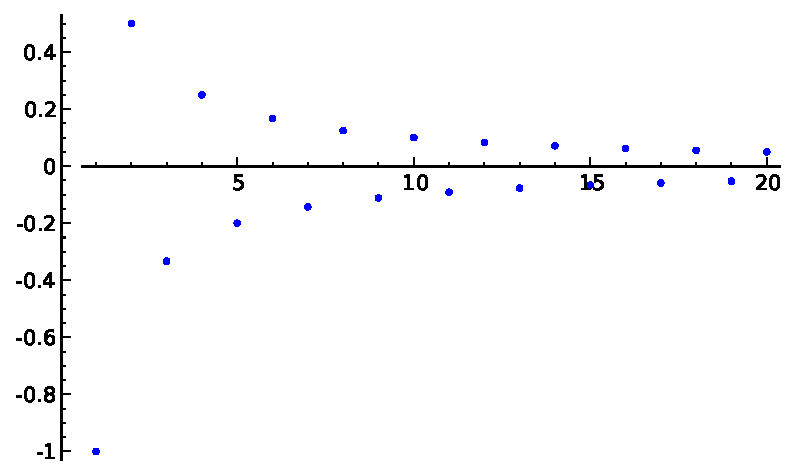
\includegraphics[width=9.5cm]{folge.pdf}
\end{center}

KONV KRIT


 Jede monotone, beschränkte Folge konvergiert.
 Konvergenz bei Addition: Sind $(a_n)_n$ und $(b_n)_n$ konvergente Folgen, $\alpha, \beta \in \mathbb{R}$, so ist auch die
                   Folge $( \alpha a_n+\beta b_n)_n$ konvergent mit
                   dem Grenzwert
 \[ \lim_{n \rightarrow \infty} ( \alpha a_n + \beta b_n)= \alpha
                   \lim_{n \rightarrow \infty} a_n + \beta \lim_{n
                   \rightarrow \infty} b_n .\]
 Konvergenz bei Multiplikation: Sind $(a_n)_n$ und $(b_n)_n$ konvergente Folgen, so ist auch die
                   Folge $(a_n b_n)_n$ konvergent mit
                   dem Grenzwert
 \[
  \lim_{n \rightarrow \infty} ( a_n b_n)= 
                   (\lim_{n \rightarrow \infty} a_n) \cdot  (\lim_{n
                   \rightarrow \infty} b_n).
 \]
 Bemerkung: Weglassen oder Hinzufügen endlich vieler Glieder verändert das
                   Konvergenzverhalten nicht.


SÄTZE


 \emph{(Bolzano-Weierstrass)}: Jede beschränkte Folge besitzt (mindestens) eine
konvergente Teilfolge.
 Jede Teilfolge einer konvergenten Folge konvergiert gegen den
Grenzwert der ursprünglichen Folge.
 Jede konvergente Folge ist beschränkt, d.h. es gibt ein $K>0$,
so dass $|a_n|\leq K$ gilt für alle $n \in \mathbb{N}$.
 \emph{Zwischenfolge}: Seien $(a_n)_n$ und $(b_n)_n$ konvergente Folgen mit $\lim_{n
\rightarrow \infty} a_n = \lim_{n \rightarrow \infty} b_n$. Dann gilt
für eine Folge $(c_n)_n$ mit $a_n \leq c_n \leq b_n$, $n \in
\mathbb{N}$, dass sie konvergiert mit  $\lim_{n
\rightarrow \infty} c_n = \lim_{n \rightarrow \infty} b_n$.


REK

Rekursive Folgen können durch rekursive Funktionen erzeugt werden.
\textbf{Beispiel:}
\[ y_{n+2}:=2y_{n+1}-y_n+2, \quad y_0=-1, y_1=a. \]
\begin{sagein}
var('a')
def y(n):
   if n==0:
       return -1
   if n==1:
       return a
   return 2*y(n-1)-y(n-2)+2
y(4)
\end{sagein}
\begin{sage}
4*a + 15
\end{sage}

%%%%%%%%%%%%%%%%%%%%%%%%%%%%%%%%%%%%%%
\section{Reihen}
%%%%%%%%%%%%%%%%%%%%%%%%%%%%%%%%%%%%%%
Sei $(a_n)_n$ eine Folge reeller Zahlen. Eine {\color{red} (unendliche)
Reihe} mit den {\color{red} Gliedern} $a_n$, in Zeichen
\[ \sum_{n=1}^\infty a_n =a_1 + a_2 + a_3 + \dots, \]
ist definiert durch die Folge $(s_n)_n$ der {\color{red} Partialsummen}\\
\[
s_n=\sum_{k=1}^n a_k = a_1+a_2+ \dots +a_n 
\]
Der Grenzwert $s$ der Folge $(s_n)_n$ wird als {\color{red} Wert} oder 
{\color{red} Summe} der Reihe bezeichnet. Man schreibt
\[s= \sum_{n=1}^\infty a_n.\] 

BEMERKUNGEN


  Reihen sind eine spezielle Art von Folgen.
 Indizierung mit $m$: $\sum_{n=m}^\infty a_n$.
 Bei Abänderung, Weglassen oder Hinzufügen endlich vieler Glieder
bleiben Konvergenz und Divergenz unberührt. I.A. wird sich aber der
Grenzwert ändern.


inSAGE

\begin{sagein}
sum(<f>,<i>,<a>,<b>) 
\end{sagein}
Gesucht: geschlossene Darstellung der Summe $\sum_{i=a}^b f(i)$ mit $a,b \in \mathbb{Z}$ ganze
Zahlen (auch unendlich (\isage{infinity/oo}), \isage{f} Ausdruck in $i$.

 Oft ist die Konvergenz einer Reihe abhängig von bestimmten Parametern. Je nach Parameterwert zeigt die Reihe
unterschiedliches Konvergenzverhalten.
%geometrische Reihe z.b.


BEISPIELE


 \emph{geometrische Reihe}: $\sum_{n=0}^\infty x^n$. Die
Partialsummen lauten
\[ s_n=1+x+x^2+\ldots + x^n = \left \{ \begin{array}{ll}
n+1, & \mbox{ falls } x=1\\
\frac{1-x^{n+1}}{1-x}, & \mbox{ falls } x \neq 1 
\end{array} \right. .\]
Die Reihe divergiert für $|x|\geq1$ und konvergiert für $|x|<1$ mit
dem Wert $\sum_{n=0}^\infty = \frac{1}{1-x}$.

\begin{sagein}
sum(x^k,k,0,oo)
\end{sagein}
\begin{sage}
Is  abs(x)-1  positive, negative, or zero?
\end{sage}
Entsprechend gibt es keine geschlossene Form. Für $x=1/2$ gilt
\begin{sagein}
x = 1/2; sum(x^k,k,0,oo)
\end{sagein}
\begin{sage}
  2
\end{sage}
 Die Reihe $\sum_{n=1}^\infty \frac{1}{n^2}$ konvergiert gegen
$\pi^2/6$.
\begin{sagein}
_=var('k');sum(1/k^2,k,1,oo)
\end{sagein}
\begin{sage}
1/6*pi^2
\end{sage}
 Die \emph{alternierende harmonische Reihe}  $\sum_{n=1}^\infty
\frac{(-1)^{n+1}}{n}$ konvergiert.
\begin{sagein}
sum((-1)^(k+1)/k,k,1,oo)
\end{sagein}
\begin{sage}
  log(2)
\end{sage}
 Die \emph{harmonische Reihe} $\sum_{n=1}^\infty \frac{1}{n}$
 divergiert.
\begin{sagein}
sum(1/k,k,1,oo)
\end{sagein}
\begin{sage}
ValueError: Sum is divergent
\end{sage}


PARTIALSUMMEN


 Definieren der Partialsumme
\begin{sagein}
_=var('x,n,k')
s = sum(x^k,k,0,n); s
\end{sagein}
{\color{blue}\[\frac{x^{{\left(n + 1\right)}} - 1}{x - 1}\]}
% \begin{sage}
% (x^(n + 1) - 1)/(x - 1)
% \end{sage}

 Die ersten $5$ Glieder der Partialsumme
\begin{sagein}
assume(x<>1); [s(n=m) for m in [1..6]]
\end{sagein}
{\color{blue}\[\left[\frac{x^{2} - 1}{x - 1}, \frac{x^{3} - 1}{x - 1}, \frac{x^{4} - 1}{x - 1}, \frac{x^{5} - 1}{x - 1}, \frac{x^{6} - 1}{x - 1}, \frac{x^{7} - 1}{x - 1}\right] \]}
% \begin{sage}
% [(x^2 - 1)/(x - 1), (x^3 - 1)/(x - 1), (x^4 - 1)/(x - 1), (x^5 - 1)/(x -
% 1), (x^6 - 1)/(x - 1), (x^7 - 1)/(x - 1)]
% \end{sage} 
 Bestimmen des Grenzwertes der Folge der Partialsummen
\begin{sagein}
forget();assume(abs(x)<1);limit(s,n=oo)
\end{sagein}
\begin{sage}
-1/(x - 1)
\end{sage}
\begin{sagein}
forget();assume(x>1);limit(s,n=oo)
\end{sagein}
\begin{sage}
+Infinity
\end{sage}
 

assume()

\begin{sagein}
assume(<assumptions>)
\end{sagein}
Annahmen für bestimmte Bezeichner.

\textbf{Beispiele:}
\begin{sagein}
assume(x,'real') # §$x$§ wird auf §$\mathbb{R}$§ eingeschränkt
assume(x>a) # §$x$§ wird auf  §$\{y \in \mathbb{R}\ |\ y>a\}$§ eingeschränkt
\end{sagein}

Ruft man \isage{assume} mehrmals für einen Bezeichner auf, werden zusätzliche Annahmen gemacht. Sind diese
Widersprüchlich erhält man eine entsprechende Meldung.

BEMERKUNGEN


 Umformungen oder Vereinfachungen für symbolische Bezeichner
werden i.A. nur dann durchgeführt,
wenn sie für alle komplexen Zahlen gelten. Hier kann ein Einschränken
des Definitionsbereichs helfen.
 Mittels 
\begin{sagein}
forget(x>a)
\end{sagein}
wird die Annahme \isage{x>a} gelöscht.
 Durch 
\begin{sagein}
assumptions() 
\end{sagein}
können alle Annahmen ausgegeben werden.
% Durch den speziellen Bezeichner \isage{Global} können Annahmen
%für alle Bezeichner gesteuert werden. 


BEISPIELE

\begin{sagein}
var('c'); assumptions()
\end{sagein}
\begin{sage}
c
[]
\end{sage}

\begin{sagein}
c = 2; assume(c>0)
\end{sagein}
\begin{sage}
 AttributeError: 'bool' object has no attribute 'assume'
\end{sage}
\begin{sagein}
_=var('c')
assume(c,'integer'); assumptions()
\end{sagein}
\begin{sage}
[c is integer]
\end{sage}
\begin{sagein}
sin(c*pi)
\end{sagein}
\begin{sage}
sin(pi*c)
\end{sage}
\begin{sagein}
sin(c*pi).simplify()
\end{sagein}
\begin{sage}
   0
\end{sage}
\begin{sagein}
assume(x>0)
sqrt(x^2).simplify()
\end{sagein}
\begin{sage}
  x
\end{sage}


% integer,
% noninteger, even, odd, rational, irrational, real, imaginary, complex,
% analytic, increasing, decreasing, oddfun, evenfun, posfun, constant,
% commutative, lassociative, rassociative, symmetric, antisymmetric,
% integervalued, one_to_one
\begin{center}
 \begin{tabular}{|l|l|}
\hline
Annahme & Erklärung\\
\hline
\isage{'real'} & $\mathbb{R}$ \\
\isage{'rational'} & $\mathbb{Q}$\\
\isage{'integer'} &  $\mathbb{Z}$\\
\isage{'complex'} & $\mathbb{C}$\\
\isage{'even'}   & gerade Zahl \\
\isage{'odd'} & ungerade Zahl\\
\isage{'increasing'} & wachsend \\
\isage{'analytic'} & analytisch\\
\hline
\end{tabular}
\end{center}

KONV KRIT


 \emph{Cauchykriterium:} Eine Reihe $\sum_{n=1}^\infty a_n$ konvergiert
                  genau dann, wenn es zu jedem $\varepsilon>0$ ein $n_0
                  \in \mathbb{N}$ gibt, so dass für alle $m,n \geq n_0$
                  gilt $| \sum_{k=m}^n a_k|<\varepsilon$.
 \emph{Notwendiges Kriterium:} Konvergiert eine Reihe, so bilden ihre Glieder eine Nullfolge. Dieses Kriterium ist \emph{nicht} hinreichend!
 \emph{Verdichtungskriterium:} Eine Reihe $\sum_{n=1}^\infty a_n$ mit
                  einer Folge nichtnegativer, monoton fallender
                  Glieder konvergiert genau dann, wenn die Reihe
                  $\sum_{n=1}^\infty 2^n a_{2^n}$ konvergiert.

Gilt $0 \leq c_n \leq a_n \leq b_n$ für alle $n \in \mathbb{N}$

  {\color{red} Minorante}: $\sum_{n=1}^\infty c_n$
  {\color{red} Majorante}: $\sum_{n=1}^\infty b_n$ 

Die Reihe $\sum_{n=1}^\infty a_n$ \emph{konvergiert}, wenn...
\begin{description}
\item[Majorantenkriterium:] eine konvergente Majorante besitzt (nichtnegative Glieder).

\item[Quotientenkriterium:] Die Glieder positiv sind und ein $q<1$
existiert, so dass für $n \in \mathbb{N}$ gilt $\frac{a_{n+1}}{a_n}
\leq q$. 
\item[Wurzelkriterium:] Die Glieder positiv sind und ein $q<1$
existiert, so dass für $n \in \mathbb{N}$ gilt $\sqrt[n]{a_n} \leq
q$. 
\item[Leibnizsches Kriterium:] wenn die Folge $(a_n)_n$ bei $\sum_{n=1}^\infty (-1)^n a_n$
eine monoton fallende  Nullfolge ist.
\end{description}
Die Reihe $\sum_{n=1}^\infty a_n$ \emph{divergiert}, wenn...
\begin{description}
\item[Majorantenkriterium:] sie eine divergente Minorante besitzt.
\end{description}

BEISPIELE


 Betrachte $\sum_{n=0}^\infty n^4 e^{-n^2}$
\begin{sagein}
f(n) = n^4*exp(-n*n)
g(n) = f(n+1)/f(n)
limit(g(n),n=oo)
\end{sagein}
\begin{sage}
  0
\end{sage}
 Betrache $\sum_{n=2}^\infty \frac{1}{n (\log n)^2}$
\begin{sagein}
f(n) = 1/(n*(log(n)^2))
g(n) = 2^n*f(2^n)
h(n) = 2^n*g(2^n)
limit(h(n+1)/h(n),n=oo)
\end{sagein}
\begin{sage}
  1/2
 \end{sage}


ABS BED KONV

{\color{red} absolut konvergent}: Ist eine Reihe $\sum_{n=0}^\infty a_n$ 
genau dann wenn $\sum_{n=0}^\infty |a_n|$ konvergiert. 

{\color{red} bedingt konvergent}: konvergent, aber nicht absolut konvergent.

 Absolut konvergente Reihen können beliebig umgeordnet werden.
 Dies ist i.d.R. bei nicht absolut konvergenten Reihen falsch!


%%%%%%%%%%%%%%%%%%%%%%%%%%%%%%%%%%%%%%
\section{Potenzreihen}
%%%%%%%%%%%%%%%%%%%%%%%%%%%%%%%%%%%%%%
{\color{red} Potenzreihe}:
\[ \sum_{n=0}^\infty a_n (x-x_0)^n \]
mit $x_0 \in \mathbb{R}$. 

{\color{red} Konvergenzradius}: 
\[  \rho := \frac{1}{ \limsup_{n \rightarrow \infty} \sqrt[n]{|a_n|}}
\]
Ist $a_n \neq 0$ für alle $n > n_0$:
\[
 \rho = \limsup_{n \rightarrow \infty} \frac{|a_{n}|}{|a_{n+1}|}.
\]

Konvergenzverhalten:

  konvergiert absolut für $|x -x_0|< \rho$.
  divergiert für $|x-x_0|>\rho$.
 Die Konvergenz an den Stellen $x_0-\rho$ und $x_0+\rho$ muss bei
jeder Reihe individuell geprüft werden.   


BEISPIELE


 $\sum_{n=1}^\infty \frac{x^n}{n!}$
\begin{sagein}
f(n) = 1/factorial(n)
rho = limit(expand(f(n)/f(n+1)),n=oo); rho
\end{sagein}
\begin{sage}
+Infinity
\end{sage}
Die Potenzreihe konvergiert für alle $x \in \mathbb{R}$. 
 $\sum_{n=0}^\infty n^s x^n$, $s>0$
\begin{sagein}
_=var('s');f(n)= n^s; assume(s>0)
limit(expand(f(n)^(1/n)),n=infinity)
\end{sagein}
\begin{sage}
  1
\end{sage}
Der Konvergenzradius ist $1$.


EXP

Wir erklären die \emph{Exponentialfunktion} durch
\[  exp(x) := \sum_{i=0}^\infty \frac{x^n}{n!}= 1 + \frac{x}{1!} +
\frac{x^2}{2!}+ \frac{x^3}{3!}+ \dots, x \in \mathbb{R}. \]
 Die Funktion ist auf ganz $\mathbb{R}$ definiert. Plot:
\begin{sagein}
plot(exp,(-5,5))
\end{sagein}
\begin{center}
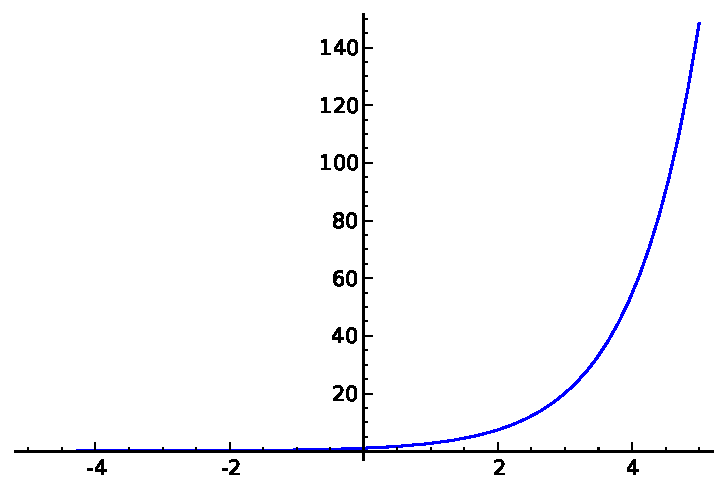
\includegraphics[width=6cm]{fexp.pdf}
\end{center}

EIG EXP


 Es gilt $\exp(x+y)=\exp(x) \cdot \exp(y)$.
 Es gilt $\exp(x)=\lim_{n \rightarrow \infty} (1+\frac{x}{n})^n$.
 Es gilt $\exp(x)=1/\exp(-x)$.
 Die Umkehrfunktion auf $\mathbb{R}_+$ der Exponentialfunktion ist die
Logarithmusfunktion $\log (x)$. Es gilt
\[ \exp(\log(x))=x, \ x >0, \quad \log ( \exp ( x ))=x, \ x \in \mathbb{R}.\] 
 Die {\color{red} allgemeine Potenz} ist durch $a^x:=\exp( x \log a)$,
$a\in \mathbb{R}_+$
definiert. 


inSAGE

\begin{sagein}
sum(x^n/factorial(n),n,0,oo)
\end{sagein}
\begin{sage}
  e^x
\end{sage}
\begin{sagein}
exp(log(x))
\end{sagein}
\begin{sage}
  x
\end{sage}
\begin{sagein}
_=var('n');limit((1+x/n)^n,n=oo)
\end{sagein}
\begin{sage}
  e^x
\end{sage}
% \begin{sagein}
% ??
% ??
% \end{sagein}
% \begin{sage}
%   
% \end{sage}

TRIG

Die {\color{red} Sinusfunktion} und die {\color{red} Cosinusfunktion} sind definiert
durch
\begin{eqnarray*}
\sin(x) := \sum_{n=0}^\infty (-1)^n \frac{x^{2n+1}}{(2n+1)!} \quad\quad
\cos(x) := \sum_{n=0}^\infty (-1)^n \frac{x^{2n}}{(2n)!}. 
\end{eqnarray*}
Die Potenzreihen konvergieren für alle $x \in \mathbb{R}$. Plotten:
\begin{sagein}
p = plot(sin,0,4*pi,color='red')
p += plot(cos,0,4*pi); 
p += text('-- $\sin(x)$', (10, 1.0), color='red')
p += text('-- $\cos(x)$', (10, 0.85)); p.show()
\end{sagein}
\begin{center}
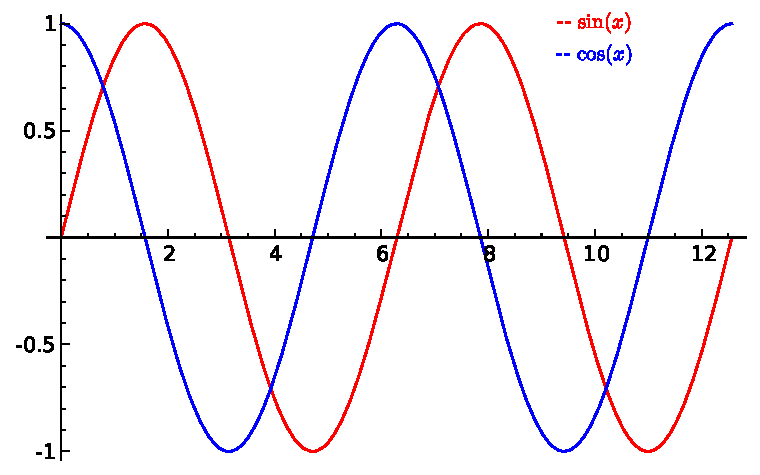
\includegraphics[width=5.5cm]{sincos.pdf}
\end{center}

EIG TRIG


 \emph{Additionstheoreme}:
\begin{eqnarray*}
\sin(x+y) & = &\sin x \cos y+ \cos x \sin y \\
\cos(x+y) & = &\cos x \cos y - \sin x \sin y .
\end{eqnarray*} 
 
\[\sin^2x +\cos^2x=1.\]
 
\begin{eqnarray*}
\sin(x+\pi/2)&=&\cos(x)\\
 \cos(x+\pi/2)&=&-\sin(x).
\end{eqnarray*} 
 Wir definieren $\pi$, indem wir die kleinste positive Nullstelle
von $\cos(x)$ als $\pi/2$ definieren.



inSAGE

\begin{sagein}
solve(cos(x)==0,x)
\end{sagein}
\begin{sage}
[x == 1/2*pi]
\end{sage}
\begin{sagein}
sin(x+pi/2).simplify()
\end{sagein}
\begin{sage}
cos(x)
\end{sage}

MORE EIG


% Man kann die Sinusfunktion und die Cosinusfunktion mit Hilfe eines rechtwinkligen Dreiecks im Einheitskreis auch geometrisch  deuten.
 Umkehrfunktionen: $\arcsin$ bei Sinus und $\arccos$ bei Cosinus.
Plotten: 
\begin{sagein}
p = plot(arcsin,-1,1,color='red')
p += plot(arccos,-1,1); 
p += text('-- arcsin(x)', (-0.7, 1.0), color='red')
p += text('-- arccos(x)', (-0.7, 0.75)); p.show()
\end{sagein}
\begin{center}
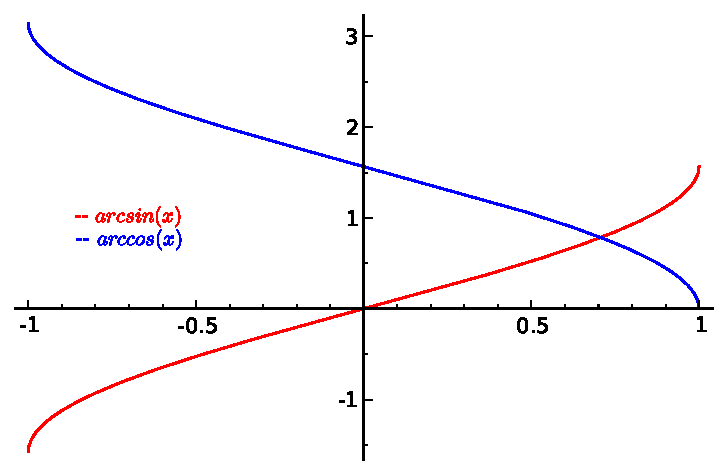
\includegraphics[width=6.5cm]{arcsinarccos.pdf}
\end{center}
 Der {\color{red} Tangens} ist definiert durch
$\tan(x) :=\frac{\sin(x)}{\cos(x)}$.
\begin{sagein}
plot(tan,-4,4,detect_poles=True,ymax=4,ymin=-4)
\end{sagein}
\begin{center}
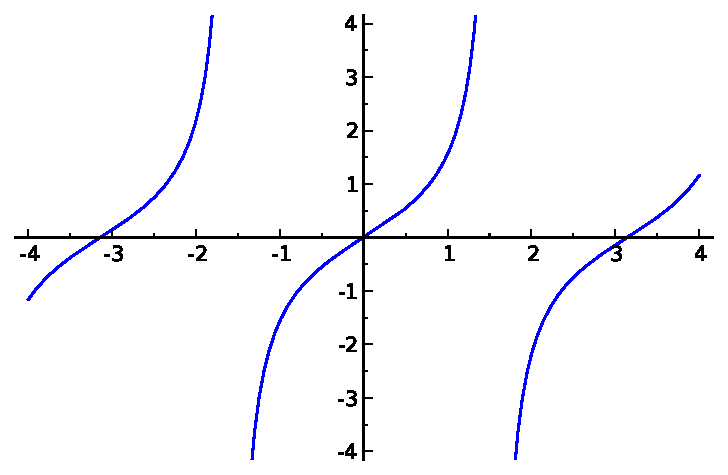
\includegraphics[width=7cm]{tan.pdf}
\end{center}


%%%%%%%%%%%%%%%%%%%%%%%%%%%%%%%%%%%%%%
\section{Vertiefung Schleifen}
%%%%%%%%%%%%%%%%%%%%%%%%%%%%%%%%%%%%%%

WHILE

\begin{sagein}
while <expression> :
    <Code-block>
\end{sagein}
Diese wiederholt \isage{<Code-block>} solange wie die \isage{<expression>} als 
\isage{True} ausgewertet wird.

\textbf{Beispiel}:
\begin{sagein}
f(x) = 1/x
x=0.1
while f(x) > 0.1:
    x += 0.1
x
\end{sagein}
\begin{sage}
 10.1000000000000
\end{sage}
%achtung: rundungsfehler, daher kommt 10.1 raus.. selbst einmal drauf reingefallen..

% 
%  Die Schleifenvariable $k$ durchläuft die Werte $1$, $2$, $3$ und
%   $4$. Dabei wird alles was ab \isage{:} eingerückt ist $k$-mal durchlaufen.
%  Ergebnisse, die in jedem Schleifenschritt berechnet werden,
%   werden \alert{nicht} auf dem Bildschirm ausgegeben. 
%  Eine Ausgabe wird durch den \isage{print}-Befehl erzielt.
% 
% \end{frame}

% \begin{frame}[fragile]{Schleifen III}
%  Eine elegante Möglichkeit sind Schleifen über Listen oder Mengen.
% \begin{sage}
% L = [1..10]
% for i in L:
%     x = i^2
%     print("Das Quadrat von {0} ist {1}").format(i,x)
% \end{sage}
% \end{frame}


% \begin{frame}[fragile]{Etwas Zahlentheorie}
% Wir geben für die natürlichen Zahlen $\leq 1000$ an, wieviele Zahlen
% $1,2,3,\dots $ Teiler haben.
% \begin{sagein}
% Liste = [1..1000]
% def anz_teiler(n): return len(divisors(n))
% Liste2 = map(anz_teiler,Liste)
% for k in [1..50]:
%     print "{0} , {1}".format(k,len(filter(lambda x: x == k, Liste2)))
% print divisors(840)
% \end{sagein}

ALT


 Schleifen abwärts zählen
\begin{sagein}
for j in reversed([2,4]):
   print("{0}, {1}").format(x,x^j) 
\end{sagein}
 Schrittweite modifizieren
\begin{sagein}
for j in srange(3,10,2.6):
    print(x,x^j) 
\end{sagein}
\begin{sage}
(x, x^3.00000000000000)
(x, x^5.60000000000000)
(x, x^8.20000000000000)
\end{sage}



FP

Suche ein $x_{\mathrm{fix}} \in \mathbb{R}$ so dass
\[ x_{\mathrm{fix}} = \cos (x_{\mathrm{fix}}) \]
gilt.
\begin{center}
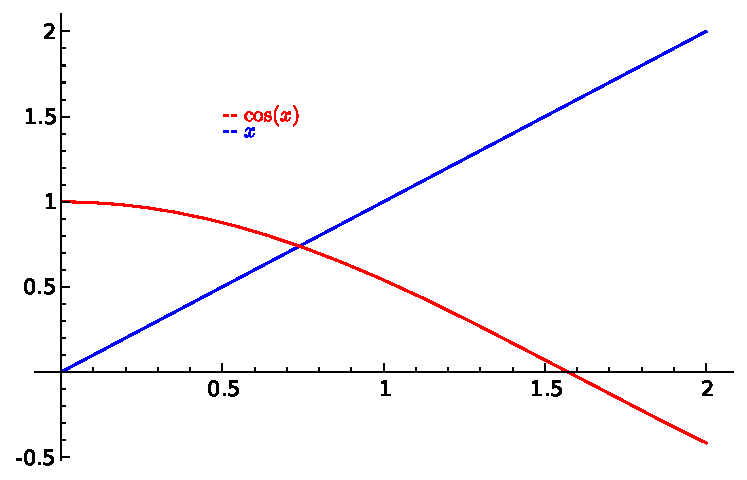
\includegraphics[width=8cm]{iter1.pdf}
\end{center}

FP-IT

Fixpunkt-Iteration 
\[ x_{k+1}=cos(x_k) \]
bei geeignetem Startwert $x_0 = 0.2$.  \\
\centering{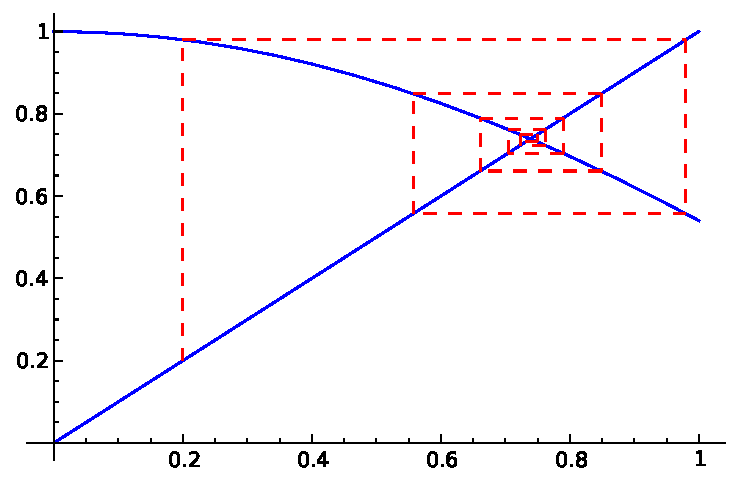
\includegraphics[width=8cm]{fixpunkt.pdf}}\\

IMP

\begin{small}
\begin{sagein}
def fixpunkt(f,In,x0,n):
    y = [x0]
    p = plot(f,(In[0],In[1]))
    p += plot(x,(In[0],In[1]))
    for i in [0..n-1]:
        y.append(float(f(y[i])))
        p += line( [ (y[i],y[i]), (y[i],y[i+1]) ],linestyle='--', color='red')
        p += line( [ (y[i],y[i+1]), (y[i+1],y[i+1]) ],linestyle='--', color='red')
    p.show()
    return(y)
\end{sagein}
\end{small}

CALL

\begin{sagein}
fixpunkt(lambda x: cos(x),[0,1],0.2,10)
\end{sagein}
\begin{sage}
[0.200000000000000, 0.98006657784124163, 0.55696725280964243, 0.84886216565827077, 0.66083755111661502, 0.78947843776686832, 0.70421571334199318, 0.76211956176066087, 0.72337417210557109, 0.74957657633149311, 0.73197742525819132]
\end{sage}


%%%%%%%%%%%%%%%%%%%%%%%%%%%%%%%%%%%%%%
\chapter{Funktionen(-folgen), Grenzwert und Stetigkeit, Grafik}
\section{Funktionen}
%%%%%%%%%%%%%%%%%%%%%%%%%%%%%%%%%%%%%%

FKT

(reelle) {\color{red} Funktion}:  Abbildung
\[f: \ D \subset \mathbb{R} \ \rightarrow \ \mathbb{R}.\]
die jedem Element aus $D$ eindeutig genau ein Element aus $\mathbb{R}$ zuordnet.

  {\color{red} Definitionsbereich}: $D \subset \mathbb{R}$, $D \neq \emptyset$.
 \emph{Wertebereich}: Die Menge $f(D)$ aller rellen Zahlen, die als Werte der
Funktion vorkommen.
 {\color{red} Graph} einer Funktion: ist die Menge aller Punkte 
\[ \{ (x,f(x)) \in \mathbb{R}^2 \;|\; x \in D\}. \]


VERK

Seien $f$ und $g$ Funktionen mit einem gemeinsamen Definitionsbereich. Dann
definiert man:

 Summe: $(f+g)(x):=f(x)+g(x)$
 Differenz: $(f-g)(x):=f(x)-g(x)$
 Produkt: $(f\cdot g)(x):=f(x) \cdot g(x)$
 Quotient: $(\frac{f}{g})(x):=\frac{f(x)}{g(x)}$, falls $g(x) \neq
0$ für alle $x \in D$ 
 Komposition: Mit $f:D_f \rightarrow \mathbb{R}$ und $g:D_g \rightarrow \mathbb{R}$
mit $f(D_f) \subset D_g$ 
\[(g \circ f) (x):=g(f(x)).\] 


MEHRDIM

Ist $D \subseteq \mathbb{R}^n$ und $f : D \Rightarrow \mathbb{R}$ dann spricht man von
einer reellen Funktion in \emph{mehreren Veränderlichen}. Das Studium dieser Funktionen ist einer der Hauptinhalte der Diff2-Vorlesung.

\bigskip

Weiterhin können Funktionen auch Wertebereiche außerhalb der reellen Zahlen haben.
Z.B. 
\[f : D \Rightarrow \mathbb{R}^m.\]
 Im physikalischen Umfeld spricht man für $m=1$ dann von \emph{skalarwertigen Funktionen} und für $m>1$ von \emph{vektorwertigen Funktionen} oder \emph{Vektorfeldern}.
 
inSAGE

\begin{sagein}
f(x,y,...) = expr
\end{sagein}
Abbildung $f$ mit Argumente $x,y$.\\
\textbf{Beispiele:}
\begin{sagein}
f(x,y) = x^2+y^2; f
\end{sagein}
\begin{sage}
(x, y) |--> x^2 + y^2
\end{sage}
Die so definierte Funktion $f$ kann wie jede beliebige andere Funktion
aufgerufen werden. Funktionen haben den Datentyp \isage{expression}.
\begin{sagein}
_=var('a,b');f(a,b+1)
\end{sagein}
\begin{sage}
(b + 1)^2 + a^2
\end{sage}
\begin{sagein}
type(f)
\end{sagein}
\begin{sage}
<type 'sage.symbolic.expression.Expression'>
\end{sage}

Wie gewohnt können Abbildungen addiert, subtrahiert, multipliziert und
dividiert werden:
\begin{sagein}
f(x) = 1/(1+x); g(x) = sin(x^2)
h = f+g; k = f*g; l = f/g
h(a),k(a),l(a)
\end{sagein}
{\color{blue} \[\left(\frac{1}{a + 1} + \sin\left(a^{2}\right),
\frac{\sin\left(a^{2}\right)}{a + 1}, \frac{1}{{\left(a + 1\right)}
\sin\left(a^{2}\right)}\right)\]}
% \begin{sage}
% (1/(a + 1) + sin(a^2), sin(a^2)/(a + 1), 1/((a + 1)*sin(a^2)))
% \end{sage}

KOMP

Kompositionen $f\circ g$ werden in Sage durch Ineinanderschachteln gelöst:
\begin{sagein}
f_g(x) = f(g); g_f(x) = g(f)
f_g(x), g_f(x)
\end{sagein}
{\color{blue} \[ \left(\frac{1}{\sin\left(x^{2}\right) + 1}, \sin\left(\frac{1}{{\left(x
+ 1\right)}^{2}}\right)\right) \]}
% \begin{sage}
% (1/(sin(x^2) + 1), sin((x + 1)^(-2)))
% \end{sage}
Mehrfaches Hintereinanderschalten $f(f(\cdots f(\cdot)))=f \circ \dots
\circ f(\cdot)$
\begin{sagein}
g4(x) = g(g(g(g))); g4
\end{sagein}
{\color{blue} \[ x \ {\mapsto}\sin\left(\sin\left(\sin\left(\sin\left(x^{2}\right)^{2}\right)^{2}\right)^{2}\right) \]}
% \begin{sage}
% x |--> sin(sin(sin(sin(x^2)^2)^2)^2)
% \end{sage}
Diese Konstruktionen funktionieren auch mit Systemfunktionen:
\begin{sagein}
abs(real(-2+3*I))
\end{sagein}
\begin{sage}
  2
\end{sage}
Kompliziertere Funktionen können besser durch selbst definierte Funktionen/Prozeduren \isage{def <func>():} erklärt
werden (vgl. Einheit 4).

AUSDR

Funktion $f$ als Funktion $f(x)=expr(x)$ oder als Ausdruck $f=expr$ (Vorsicht: der Typ ist identisch).
Funktionsauswertung ist i.A. allerdings unterschiedlich.
\begin{sagein}
Funktion(x) = 2*x*cos(x); Funktion(1)
\end{sagein}
\begin{sage}
  2*cos(1)
\end{sage}
\begin{sagein}
Ausdruck = 2*x*cos(x); Ausdruck(x=1)
\end{sagein}
\begin{sage}
  2*cos(1)
\end{sage}
Auch mehrere Veränderliche  sind möglich:
\begin{sagein}
_=var('y');Funktion2(x) = x+sin(y); Funktion2
\end{sagein}
\begin{sage}
 x |--> x + sin(y)
\end{sage}
\begin{sagein}
Funktion3(x,y) = x+sin(y); Funktion3
\end{sagein}
\begin{sage}
  (x, y) |--> x + sin(y)
\end{sage}

%%%%%%%%%%%%%%%%%%%%%%%%%%%%%%%%%%%%%%
\section{Grenzwerte und Stetigkeit}
%%%%%%%%%%%%%%%%%%%%%%%%%%%%%%%%%%%%%%

GRENZ

{\color{red} Grenzwert}: Sei $f$ eine Funktion mit Definitionsbereich $D$ und $a\in D$.\\
$f$ strebt für $x \rightarrow a$ gegen $b \in \mathbb{R}$, wenn es zu jedem $\varepsilon >0$ ein $\delta >0$ gibt, so
dass für alle $x \in D\smallsetminus\{a \}$ mit $|x-a|<\delta$ gilt 
\[ |f(x)-b| < \varepsilon .\]
Der Grenzwert $b$ ist eindeutig bestimmt und man schreibt
\[ \lim_{x \rightarrow a} f(x) =b \mbox{ oder } f(x) \rightarrow b
\mbox{ für } x \rightarrow a. \]
Die Aussage überträgt sich sinngemäß auf $a=\pm \infty$.

BEM


 \emph{Folgenkriterium}: Es gilt $ \lim_{x \rightarrow a} f(x) =b$
genau dann, wenn für jede Folge $a_n \in D$ mit $a_n \neq a$ und $a_n \rightarrow a$
gilt $\lim_{n \rightarrow \infty} f(a_n)=b$.
 Es gelten die üblichen Rechenregeln:
\begin{eqnarray*}
\lim_{x \rightarrow a}(f(x)+g(x)) &=&\lim_{x \rightarrow a} f(x) +
\lim_{x \rightarrow a} g(x) \\
\lim_{x \rightarrow a}(f(x) \cdot g(x)) &=& \lim_{x \rightarrow a}
f(x) \cdot \lim_{x \rightarrow a} g(x)
\end{eqnarray*}
wenn $\lim_{x \rightarrow a} f(x)$ und $\lim_{x \rightarrow a}g(x)$
existieren. 
 Gilt $\lim_{x \rightarrow a} f(x)=b$, $\lim_{x \rightarrow b}
g(x)=c$ bei entsprechenden Definitionsgebieten für $f$ und $g$, so
folgt $\lim_{x \rightarrow a} g(f(x)) =c$.


limit()

\begin{sagein}
expr.limit(x = a, dir=None, taylor=False)
limit(expr, x = a, dir=None, taylor=False)
\end{sagein}
Hierdurch wird der (beidseitige) Grenzwert eines Ausdrucks mit Unbekannten $x$ an
der Stelle $a$ bestimmt. $a$ kann auch $\pm \infty$ sein (\isage{infinity} oder \isage{oo}).\\

  \isage{dir='minus'}: linksseitige Limes. 
 \isage{dir='plus'}: rechtsseitige Limes.
 \isage{taylor=True}: es wird eine Taylorentwicklung benutzt. 


inSAGE


 Grenzwert $\lim_{x \rightarrow 0}
\frac{\sin(x)}{x}$
\begin{sagein}
limit(sin(x)/x,x=0)
\end{sagein}
\begin{sage}
  1
\end{sage}
 Grenzwert $\lim_{x \rightarrow \infty}
\frac{\log(x)}{x}$
\begin{sagein}
limit(log(x)/x,x=infinity)
\end{sagein}
\begin{sage}
  0
\end{sage}
 Grenzwert $\lim_{x \rightarrow \infty} \sqrt[x]{x}$
\begin{sagein}
limit(x^(1/x),x=infinity)
\end{sagein}
\begin{sage}
  1
\end{sage}
 Grenzwert $\lim_{x \rightarrow 0}
\sin(1/x)$
\begin{sagein}
limit(sin(1/x),x=0)
\end{sagein}
\begin{sage}
  ind
\end{sage}
Der Grenzwert existiert nicht: \isage{ind} (indefinite aber beschränkt). 
 Grenzwert $\lim_{x \rightarrow 0} |x|' $
\begin{sagein}
limit(diff(abs(x),x),x=0),
limit(diff(abs(x),x),x=0,dir='minus'),
limit(diff(abs(x),x),x=0,dir='plus')
\end{sagein}
\begin{sage}
  (und, -1, 1)
\end{sage}


STET

Eine Funktion $f:D \ \rightarrow  \ \mathbb{R}$ heißt {\color{red} stetig an
der Stelle $x_0 \in D$}, wenn es zu jedem $\varepsilon>0$ ein $\delta>0$
gibt, so dass für alle $x \in D$ mit $|x - x_0| < \delta$ gilt
\[ |f(x)-f(x_0) | < \varepsilon .\]
Man sagt, dass $f$ {\color{red} stetig} ist, wenn $f$ an jeder Stelle $x_0
\in D$ stetig ist. \\
Sind $f$ und $g$ an $x_0$ stetig, so auch $f+g$, $f-g$, $f \cdot g$
und $\frac{f}{g}$ (falls $g(x_0) \neq 0$). 

SÄTZE


 Sei $f$ auf einem offenen Intervall $I$ definiert. $f$ ist an
$x_0 \in I$ genau dann stetig, wenn gilt
\[ \lim_{x \rightarrow x_0} f(x) = f(x_0). \]
 Für $f:I \rightarrow \mathbb{R}$ und $g:J \rightarrow
\mathbb{R}$ gelte $f(I) \subset J$ und es seien $f$ an $x_0 \in I$ und
$g$ an $y_0=f(x_0)$ stetig. Dann ist $g \circ f$ an $x_0$ stetig.
 Eine Funktion $f: D \rightarrow \mathbb{R}$ ist {\color{red}
linksstetig} bzw. {\color{red} rechtsstetig}, wenn $f|_{D\cap (-\infty,x_0)}$
bzw  $f|_{D\cap (x_0,\infty)}$ an $x_0$ stetig ist. Eine Funktion $f$
ist dann an $x_0$ stetig, genau dann wenn $f$ links- und rechtsstetig
an $x_0$ ist.
 Eine stetige Funktion auf einem abgeschlossenen Intervall $I=[a,b]$
besitzt ein Maximum und ein Minimum.
 Eine stetige Funktion $f$ auf einem abgeschlossenen  Intervall
$[a,b]$ nimmt in $I$ jeden Wert zwischen $f(a)$ und $f(b)$ an.
 Potenzreihen $f(x)=\sum_{n=0}^\infty a_n (x-x_0)^n$ sind stetig
innerhalb ihres Konvergenzintervalls.


GLM STET

$f: D \rightarrow \mathbb{R}$ heißt {\color{red} gleichmäßig stetig auf $D$},
wenn es zu jedem $\varepsilon >0$ ein $\delta>0$ gibt, so dass für alle
Paare $x,x_0 \in D$ mit $|x - x_0|< \delta$ gilt
\[ | f(x)-f(x_0)| < \varepsilon. \]

 Die Exponentialfunktion ist auf jedem kompakten Intervall
gleichmäßig stetig (aber nicht auf ganz $\mathbb{R}$). 
 $\log:(0,1) \rightarrow \mathbb{R}$ ist stetig aber nicht
gleichmäßig stetig.


inSAGE

Stetigkeit einer Funktion $f$ an einer Stelle $x_0$: linksseitige und rechtsseitige Grenzwerte bestimmen.
\begin{sagein}
limit(1/x,x=0,dir='plus') 
\end{sagein}
\begin{sage}
 +Infinity
\end{sage}
\begin{sagein}
 limit(1/x,x=0,dir='minus')
\end{sagein}
\begin{sage}
 -Infinity
\end{sage}

%%%%%%%%%%%%%%%%%%%%%%%%%%%%%%%%%%%%%%
\section{Funktionenfolgen}
%%%%%%%%%%%%%%%%%%%%%%%%%%%%%%%%%%%%%%

FKT FOLG

Seien $f_n: D \ \rightarrow \ \mathbb{R}$, $n \in
\mathbb{N}$  rellwertige Funktionen auf  $D \subset \mathbb{R}$.

 $(f_n)_n$ heißt {\color{red} Funktionenfolge.}
 Ist für jedes $x\in D$ die Folge $(f_n(x))_n$ konvergent, so wird durch 
\[ f(x):= \lim_{n \rightarrow \infty} f_n(x), \quad x \in D \]
die {\color{red} Grenzfunktion} $f:D \ \rightarrow \ \mathbb{R}$ definiert.
 Man sagt $f_n$ strebe {\color{red} punktweise} auf $D$ gegen $f$.  
 Durch $\sum_{i=1}^\infty f_i$ definierte {\color{red} Funktionenreihen}
sind spezielle Funktionenfolgen.
  

GRENZÜ


 $x^n \rightarrow 0$ auf dem Intervall $(-1,1)$.
 $\left( 1+ \frac{x}{n} \right)^n \rightarrow \exp(x)$ auf $\mathbb{R}$.
 Potenzreihen konvergieren innerhalb ihres Konvergenzradius.
 {\color{red} Warnung} zum Vertauschen der Grenzprozesse für $x \in (0,1)$:
\[ \lim_{x \rightarrow 1} \lim_{n \rightarrow \infty} x^n =0 \neq 1 = 
  \lim_{n \rightarrow \infty} \lim_{x \rightarrow 1} x^n.\]  


GLM KONV


$(f_n)_n$ konvergiert {\color{red} gleichmäßig} auf $D$ gegen $f$, wenn es zu
jedem $\varepsilon >0$ ein $n_0 \in \mathbb{N}$ gibt, so dass für alle
$x \in D$ und $n\geq n_0$ gilt:
\[ |f_n(x) -f(x)| < \varepsilon.\]



 Konvergiert $(f_n)_n$ gleichmäßig auf $D$ und existiert $\lim_{x
\rightarrow a} f_n(x)$ für $a\in D$, so gilt:
\[ \lim_{x \rightarrow a} \lim_{n \rightarrow \infty} f_n(x) = \lim_{n
\rightarrow \infty} \lim_{x \rightarrow a} f_n(x). \]


BEM


 Die Grenzfunktion einer gleichmäßig konvergenten Folge stetiger
Funktionen ist stetig.
 \emph{Funktionenreihen}: Ist $f_1, f_2, \ldots$, eine Folge von Funktionen auf $D \subseteq \mathbb{R}$ dann definiert
\[
 s := \sum_{n=1}^\infty f_n
\]
eine Funktionenreihe. 

Alle Aussagen übertragen sich analog; ebenso die Aussagen über die Folge der Partialsummen
\[
 s_k := \sum_{n=1}^k f_n.
\]
 
 


%%%%%%%%%%%%%%%%%%%%%%%%%%%%%%%%%%%%%%
\section{Grafik}
%%%%%%%%%%%%%%%%%%%%%%%%%%%%%%%%%%%%%%



 Grafiken werden im Notebook integriert.
 3D-Grafiken können interaktiv bearbeitet werden.
 Grafikbefehle erzeugen {\color{red} grafische Objekte} wie Geraden, Funktionsgraphen oder Kurven.
 Darstellung: \isage{<grafikobjekt>.show()} (oder letzte Zeile) stellt die {\color{red} grafische
Szene} dar
 Speichern:

[2D] \isage{<grafikobjekt>.save('filename.extension')} speichert im Format \isage{<extension>}
[3D] \glqq{}Get Image\grqq{}-Link unter der Grafiken liefert Bitmap.

 es existieren eine Reihe spezialisierter Plot-Funktionen (Pfeile, Kugel, etc.)


OPT
OBJEKTE

\begin{tabular}{lp{8cm}}
\isage{linestyle}  & Darstellung von Linien
           (\isage{'-'} (solid), \isage{'-.'} (dashed), \isage{':'}) (dotted)
                {\color{blue} \isage{linestyle = '.'}}\\
\isage{thickness}  & Linienstärke in mm
              {\color{blue} \isage{thickness = 4}}\\
\isage{color}      & Zuweisung einer Farbe
              {\color{blue} \isage{color='red'}}\\
\isage{plot_points}        & Anzahl Stützstellen
              {\color{blue} \isage{plot_points  = [nx,ny]}} (2 Parameter)\\
\isage{alpha/opacity}  & Transparenzfaktor
     {\color{blue} \isage{alpha = 0.8}}\\
\end{tabular}



SZENEN

\begin{tabular}{lp{8cm}}
\isage{aspect_ratio} & Verhältnis der Achsen (Breite/Höhe). $1$ für 1:1 Verhältnis. 
              {\color{blue} \isage{aspect_ratio = 2}}\\
\isage{figsize}    & Grösse des Bildes 
                  {\color{blue} \isage{figsize = [width, height]}}\\          
\isage{axes_labels} &  Tuple oder Liste der Achsenbeschriftungen 
{\color{blue} \isage{axes_labels = ('$x$','$y$')}}\\
\isage{gridlines} & Gitterlinien
              {\color{blue} \isage{gridlines = True}}
\end{tabular}

plot()

Skalare Funktionen 
$f:\mathbb{R}^n \ \rightarrow \mathbb{R},\, n=2,3$
\begin{sagein}
plot(f2,(x,a,b),optionen,...)
plot3d(f3,(x,a,b),(y,c,d),optionen,...)
\end{sagein}
auf dem Intervall $x \in [a,b]$ bzw. $(x,y) \in [a,b] \times [c,d]$. 


 Die Angabe des Intervalls ist optional. 
 \isage{plot.options} gibt einem die Default-Optionen aus (2D)


BSP

\begin{sagein}
plot(x^2-1)
plot(sin(1/x),(x,-1,1))
plot(sin(1/x),(x,-1,1),adaptive_recursion=0)
\end{sagein}

\begin{sagein}
p = plot(sin(x),color='red',xmin=-pi,xmax=pi)
p += plot(cos(x),xmin=-pi,xmax=pi); p.show()
\end{sagein}
\begin{center}
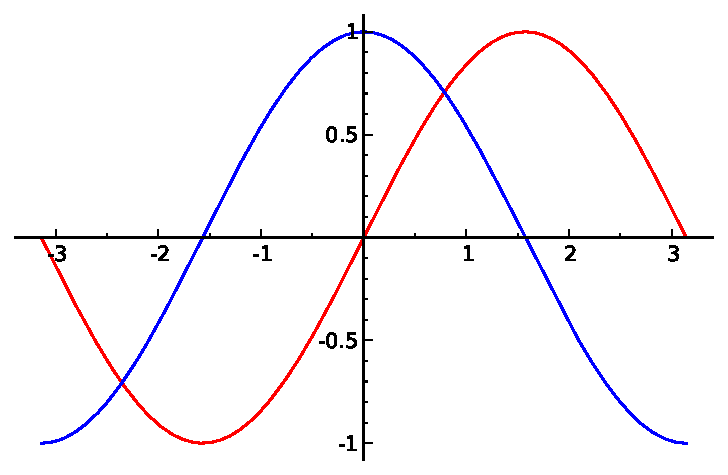
\includegraphics[width=6cm]{sincos2.pdf} 
\end{center}

Plot von $f(x,y)=\sin(y^2+x)-\cos(y-x^2)$ auf $[0,\pi]^2$:
\begin{sagein}
f(x,y) = sin(y^2+x)-cos(y-x^2)
plot3d(f,(x,0,pi),(y,0,pi))
plot3d(f,(x,0,pi),(y,0,pi),plot_points=[10,10])
\end{sagein}
\medskip
Plot von $f(x,y)=\cos (20 \exp(-x^2-y^2 ))$ auf $[-1,1] \times [-1,1]$:
\begin{sagein}
g(x,y) = cos(20*exp(-x^2-y^2))
plot3d(g,(x,-1,1),(y,-1,1))
plot3d(g,(x,-1,1),(y,-1,1),plot_points=[80,80])
\end{sagein}
\begin{center}
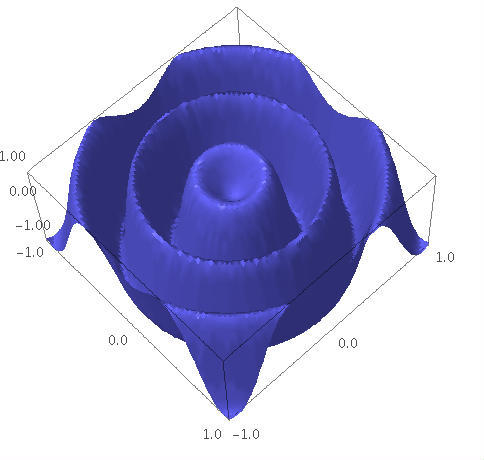
\includegraphics[width=4cm]{cosexp_trim.jpg} 
\end{center}

\begin{sagein}
W = plot3d(sin(pi*((x)^2+(y)^2))/2,(x,-1,1),(y,-1,1), frame=False, color='purple', opacity=0.8) 
S = sphere((0,0,0),size=0.3, color='red', aspect_ratio=[1,1,1])
show(W + S, figsize=8)
\end{sagein}
\begin{center}
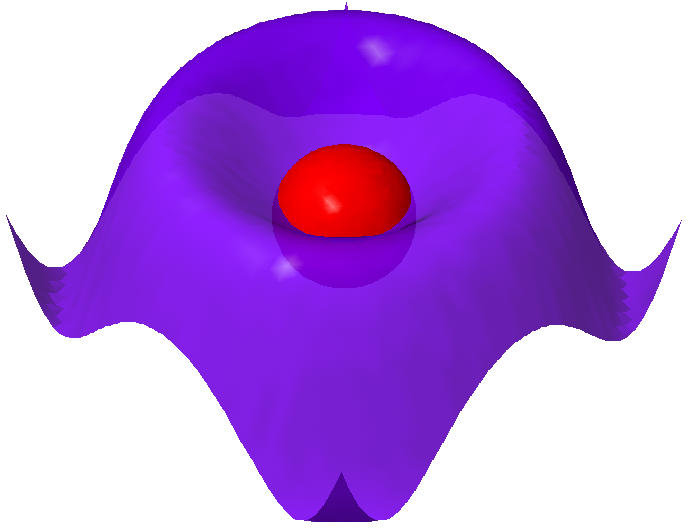
\includegraphics[width=7cm]{ball.jpg} 
\end{center}

KURV

Parameterdarstellung: 
\[
 \{(x(t),y(t)) \in \mathbb{R}^2 \;|\; t \in [a,b]\}.
\]
\[
 \{(x(t),y(t),z(t)) \in \mathbb{R}^3 \;|\; t \in [a,b] \}.
\]
%Graph einer Funktion $f(x)$, $x \in [a,b]$: $t,f(t)$ mit  $t \in [a,b]$. 
\begin{sagein}
parametric_plot([x(t),y(t)], (t,a,b), optionen, ...)
parametric_plot([x(t),y(t),z(t)], (t,a,b), optionen, ...)
\end{sagein}
%$x$, $y$ und $z$ sind Ausdrücke mit der Unbekannten $t$. 

2D KURV

\begin{sagein}
_=var('t');f1 = parametric_plot([t,sin(t)],(t,0,2*pi),color='red')
f2 = parametric_plot([t,cos(t)],(t,0,2*pi),color='green')
f3 = parametric_plot([cos(t),sin(t)],(t,0,2*pi))
(f1+f2+f3).show(figsize=7)
\end{sagein}
\begin{center}
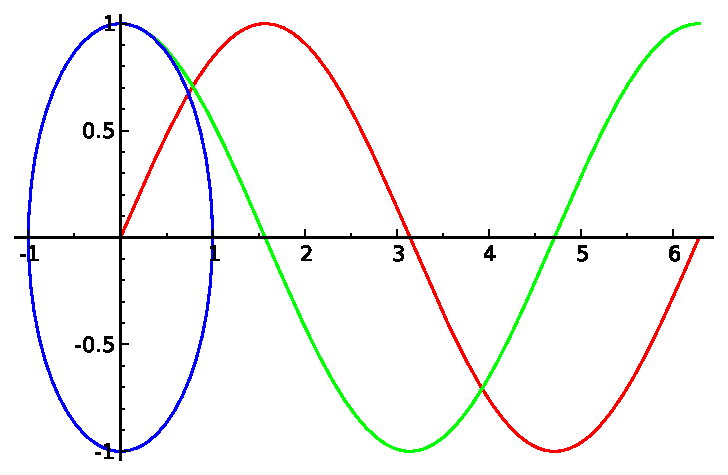
\includegraphics[width=7cm]{parametric2d.pdf} 
\end{center}

\begin{sagein}
[parametric_plot([cos(t),sin(t)],(t,0,2*pi),plot_points=2*k+1,randomize=False,adaptive_recursion=0 ) for k in [2..10]]
\end{sagein}
\begin{center}
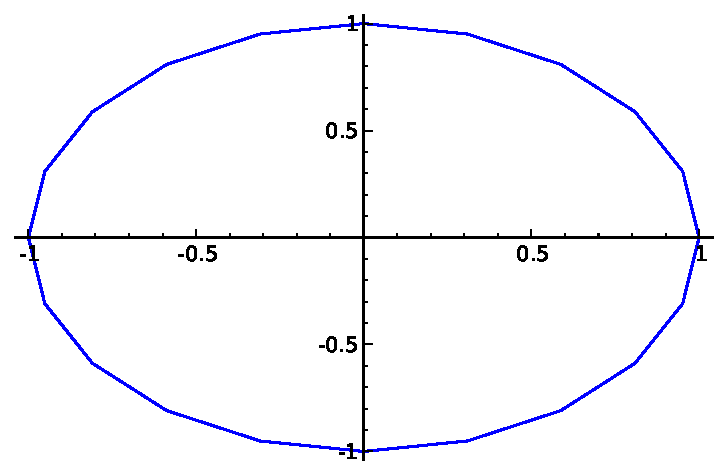
\includegraphics[width=7cm]{parametric2d_2.pdf} 
\end{center}

3D KURV

\begin{sagein}
parametric_plot([(1-t*t)*cos(99*t),(1-t*t)*sin(99*t),t], (t,0,1),plot_points=400)
\end{sagein}
\begin{center}
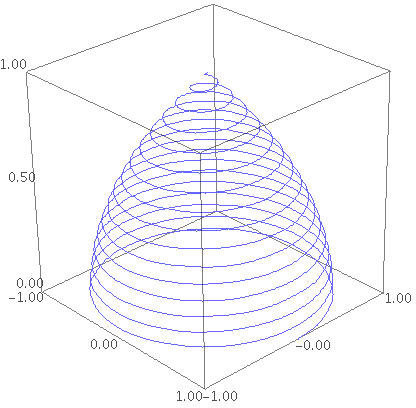
\includegraphics[width=7cm]{parametric3d.jpg} 
\end{center}

FLÄ

Fläche des $\mathbb{R}^3$ in Parameterdarstellung:
\[
 \{(x(t1,t2),y(t1,t2),z(t1,t2)) \in \mathbb{R}^3 \;|\; t1 \in [a,b], t2 \in [c,d] \}.
\]
Befehl: 
\begin{sagein}
parametric_plot([x(t1,t2), y(t1,t2), z(t1,t2)], (t1,a,b), (t2,c,d), optionen, ...)
\end{sagein}
%  Beispielsweise lassen sich Graphen von Funktionen $f:[a
%    ,b]\times [c,d]
%    \ \rightarrow \ \mathbb{R}$ als Flächen
% \[ x=t_1, \ y=t_2, \ z=f(t_1,t_2) \]
% mit $a \leq t_1 \leq b, \ c \leq
%    t_2 \leq d$ erklären.

BSP

Ellipsoid-Oberfläche
\[ 
x=r \cos(t_1) \sin(t_2), \ y=2r \sin (t_1) \sin (t_2),\ z =r \cos(t_2) 
\]
 mit $0 \leq t_1 \leq 2 \pi, 0 \leq t_2 \leq \pi.$ 
\begin{sagein}
_=var('t1,t2');r=1
x=r*cos(t1)*sin(t2)
y=2*r*sin(t1)*sin(t2)
z=r*cos(t2)
parametric_plot3d([x,y,z],(t1,0,2*pi),(t2,0,pi),aspect_ratio=1)
\end{sagein}
\begin{center}
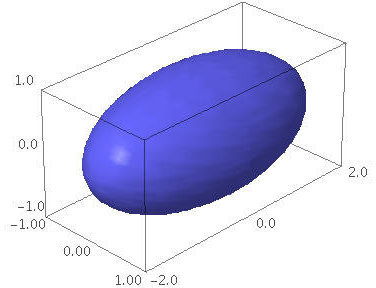
\includegraphics[width=4.5cm]{surface.jpg} 
\end{center}

KONTUR

Zweidimensionale Grafik für $f:\mathbb{R}^2 \rightarrow \mathbb{R}$:
\emph{Niveaulinien} (z.B. Höhenmeter auf einer
Landkarte):
\[ 
\{(x,y) \in \mathbb{R}^2 \;|\; f(x,y)=c, c \in \mathbb{R}\}
\]

\begin{sagein}
contour_plot(f, (x,a,b), (y,c,d), contours=[c1,c2,...], optionen, ...)
\end{sagein}
Dabei geben $c1,c2,\ldots$ die entsprechenden Niveaulinien an.

  \isage{fill=True}: Fläche zwischen den Linien ausfüllen.
  \isage{labels=True}: Automatische Kennzeichnung der Konturlinien.


BSP

Zeichnen die Niveaulinien für $-0.5, 0, 0.5$ der Funktion $\sin(4\pi x)y$. 
\begin{sagein}
contour_plot(sin(pi*4*x)*y,(x,-1,1),(y,-1,1),contours = [-0.5, 0, 0.5],fill=False,labels=True)
\end{sagein}
\begin{center}
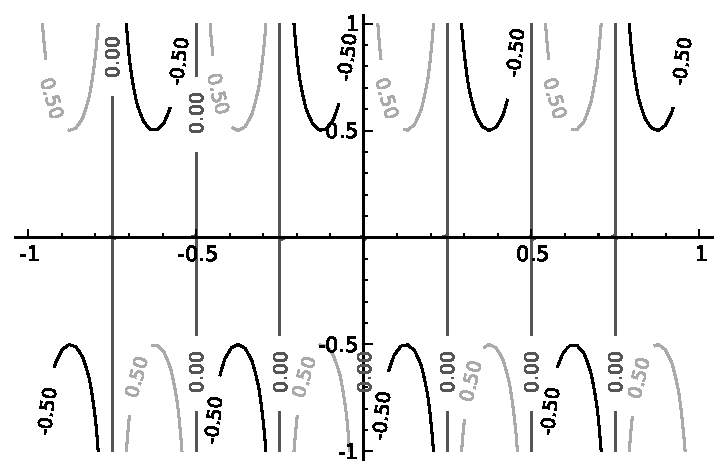
\includegraphics[width=7.5cm]{contour.pdf} 
\end{center}

paint()

Mittels {\color{blue} \isage{point}} 
können Punkte gezeichnet werden.

\textbf{Beispiel:}
\begin{sagein}
point([(i,sin(i*6.28/50)) for i in [0..50]],color='red', pointsize=30) 
point2d.options
\end{sagein}
\begin{center}
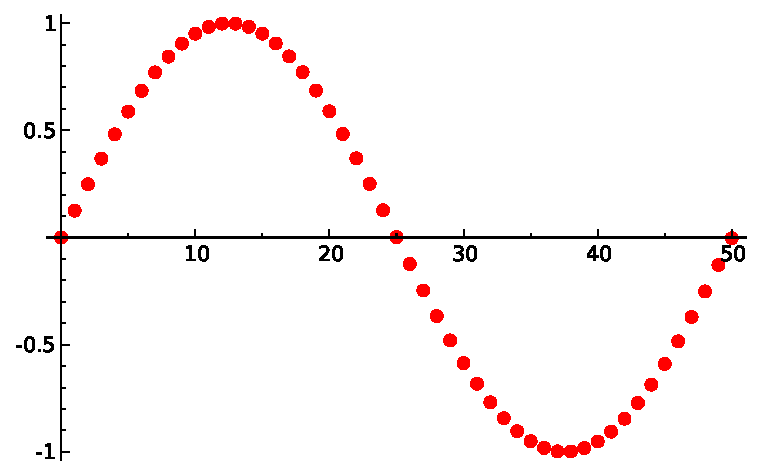
\includegraphics[width=7cm]{point2d.pdf} 
\end{center}

COLLATZ

Sei $x_0\in \mathbb{N}$. Dann definiert man die folgende Folge
\[ x_n:= \left \{ \begin{array}{ll}
 x_{n-1}/2, & \mbox{falls } x_{n-1} \mbox{ gerade ist} \\
3x_{n-1}+1 & \mbox{falls } x_{n-1} \mbox{ ungerade ist} 
\end{array} \right. . \] 
Man kann zeigen, dass für alle Startwerte ein $N_0$ existiert mit $x_{N_0}=1$.

\begin{sagein}
def collatz(n):
    """ Collatz problem """
    sequence = [n]; next_value = n;
    while next_value > 1:
        if next_value % 2 == 0:
            next_value = next_value/2
        else:
            next_value = 3*next_value+1
        sequence.append(next_value)
    Objekt = point([(i,sequence[i]) for i in [0..len(sequence)-1] ]) 
    Objekt.show()   
    return sequence
\end{sagein}
\begin{center}
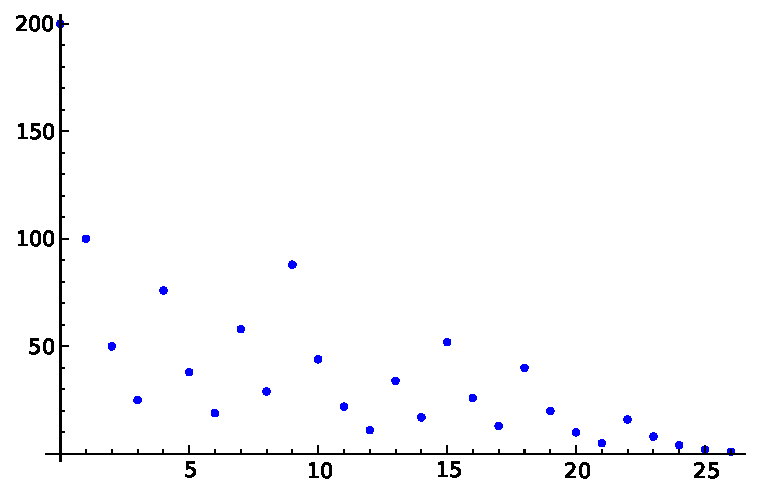
\includegraphics[width=5cm]{collatz.pdf} 
\end{center}

animate()

Der Befehl 
\begin{sagein}
animate([<graph1,graph2,...>], optionen, ... ) 
\end{sagein}
erstellt Animationen aus 2D plots. Optionen: \isage{xmin, xmax, ymin, ymax}.

\textbf{Beispiel:}
\begin{sagein}
a = animate([plot(a*x^2, (x,-5,5)) for a in [-10..10]],ymin=-100,ymax=100)
a.show(iterations=1)
\end{sagein}
\begin{center}
% \animategraphics[height=4cm]{2}{anime_}{0}{20}
\end{center}
%  Dreidimensionales Beispiel
% \begin{sagein}
% plotfunc3d(cos(j^0.5*PI*exp(-x^2-y^2)), 
%    x=-1..1, y=-1..1, j=1..30, Mesh=[40,40])
% \end{sagein}

%%%%%%%%%%%%%%%%%%%%%%%%%%%%%%%%%%%%%%
\chapter{Differentiation, Taylorsche Formel, Integration}
\section{Differentiation}
%%%%%%%%%%%%%%%%%%%%%%%%%%%%%%%%%%%%%%

DIFF

Eine Funktion $f: D \ \rightarrow \mathbb{R}$ heißt {\color{red}  differenzierbar} an
der Stelle $x_0 \in D$, wenn 
\[ \lim_{x \rightarrow x_0} \frac{f(x)-f(x_0)}{x -x_0} \]
existiert. \\
Der Grenzwert wird {\color{red} Ableitung} oder {\color{red} Differentialquotient}
von $f$ an $x_0$ genannt und mit $f\,'(x_0)=f^{\,(1)} (x_0)$ bezeichnet.

BEM


 $f$ {\color{red} differenzierbar} (auf $D$): Wenn $f$ an jeder
Stelle von $D$ differenzierbar ist. 
 {\color{red} Ableitung} von $f$: $f\,'$ für die gilt $f$ differenzierbar auf $D$.
 Eine Funktion $f:D \rightarrow \mathbb{R}$ ist an $x_0 \in D$
genau dann differenzierbar, wenn es eine lineare Abbildung
$T:\mathbb{R} \rightarrow \mathbb{R}$ gibt, so dass 
\[ f(x_0+h)=f(x_0) +Th + R(h)h, \quad \lim_{h \rightarrow 0} R(h)=0 \]
gilt ($T$ und $R$ hängen i.A. von $x_0$ ab). 
 $f$ an $x_0 \in D$ differenzierbar => stetig.


BSP


 $(x^n)'=n x^{n-1}$
 $(e^x)'=e^x$
 $(\log(x))'= \frac{1}{x}$, $x>0$
 $(\sin(x))'=\cos(x)$
 $(\cos(x))'=-\sin(x)$


LANDAU

Sei $f$ eine Funktion, die auf einem Intervall definiert ist, das $0$
enthält. 

  {\color{red} $f(x)=O(x^n)$}: Es gibt eine Kontante $C >0$, so dass
\[  \lim_{x \rightarrow 0} \frac{|f(x)|}{|x|^n} \leq C\]
($f(x)$ geht gegen $0$ mindestens so schnell wie $x^n$)
 {\color{red} $f(x)=o(x^n)$}: 
\[  
 \lim_{x \rightarrow 0} \frac{|f(x)|}{|x|^n}=0
\]
($f(x)$ geht schneller gegen $0$ als $x^n$)


HÖH ABL


 \emph{$f$ $n$-mal differenzierbar, $f^{\,(n)}$}: Ist $f:D
\rightarrow \mathbb{R}$ $(n-1)$-mal differenzierbar mit der
$(n-1)$-ten Ableitung $f^{\,(n-1)}$ und ist $f^{\,(n-1)}$ wiederum
differenzierbar.
 Ist $f$ $n$-mal differenzierbar und ist die $n$-te Ableitung $f^{\,(n)}$
stetig, so heißt $f$ $n$-mal {\color{red} stetig differenzierbar}.
 $f$ heißt {\color{red} unendlich oft differenzierbar}, wenn $f$ $n$-mal
differenzierbar ist für alle $n\in \mathbb{N}$. 


inSAGE

\begin{sagein}
diff(<Ausdruck>,x) 
\end{sagein}
wird ein Ausdruck oder eine Funktion nach $x$ abgeleitet. \\
\textbf{Beispiele:}
\begin{sagein}
diff(sin(x),x)
\end{sagein}
\begin{sage}
cos(x)
\end{sage}
\begin{sagein}
diff(x^x,x)
\end{sagein}
\begin{sage}
(log(x) + 1)*x^x
\end{sage}

\begin{sagein}
diff(<Ausdruck>,x1,x2,x3,...)
diff(<Ausdruck>,x,<anzahl>) 
\end{sagein}
Ableitung bzgl. der Unbekannten $x1$, dann der entstehende Ausdruck bzgl. $x2$, etc. 
In der 2ten Form gibt \isage{<anzahl>} die Anzahl der Ableitung bzgl. \isage{x} an.\\
\textbf{Beispiele:} 
\begin{sagein}
_=var('x,y,a'); diff(x^2*y^2+a,x,y)
\end{sagein}
\begin{sage}
4*x*y
\end{sage}
\begin{sagein}
diff(1/x,x,10)
\end{sagein}
\begin{sage}
3628800/x^11
\end{sage}

ABL BSP

\begin{sagein}
f(x) = log(cos(x))
f.diff(); diff(f); diff(f,x,x)
\end{sagein}
\begin{sage}
x |--> -sin(x)/cos(x)
x |--> -sin(x)/cos(x)
x |--> -sin(x)^2/cos(x)^2 - 1
\end{sage}
\begin{sagein}
g(x,y) = sin(x^2+y^2)
g.diff(x,x,y)
\end{sagein}
\begin{sage}
(x, y) |--> -8*x^2*y*cos(x^2 + y^2) - 4*y*sin(x^2 + y^2)
\end{sage}

REGELN

Seien $f,g:D \rightarrow \mathbb{R}$ differenzierbare Funktionen und
$x_0 \in D$. Dann gilt

 \emph{Summe}: $(f+g)'(x_0)=f\,'(x_0)+ g\,'(x_0)$
 \emph{Produktregel}: \[(f \cdot g)'(x_0) = f\,'(x_0) \cdot g(x_0) + f(x_0)g\,'(x_0)\] 
 \emph{Quotientenregel}: \[\left(\frac{f}{g}\right)'(x_0) = \frac{f\,'(x_0) g(x_0) - f(x_0)
g'(x_0)}{(g(x_0))^2}\]
falls $g(x_0) \neq 0$ .
 \emph{Kettenregel}: Seien $f:D_f \rightarrow \mathbb{R}$ und $g:D_g
\rightarrow \mathbb{R}$ mit $f(D_f) \subset D_g$. Ferner seien $f$ an
$x_0 \in D_f$ und $g$ an $y_0=f(x_0)$ differenzierbar. Dann gilt
\[ (g \circ f)(x_0) = g\,'(y_0) \cdot f\,'(x_0).  \]
 \emph{Leibnizsche Regel}:
\[
(f \cdot g)^{(n)} = \sum_{k=0}^n \binom{n}{k} f^{\,(k)} g^{\,(n-k)}.
\]
 \emph{Umkehrfunktion $f^{\,-1}$}:
\[(f^{\,-1})' \circ f = \frac{1}{f\,'}.\]


SÄTZE


Ist eine Funktion $f$ an $x_0$ differenzierbar und hat sie ein
lokales Extremum, so gilt $f\,'(x_0)=0$.

Mittelwertsatz 
Sei $f$ eine in dem Intervall $[a,b]$ stetige
und in $(a,b)$ differenzierbare Funktion. Dann gibt es ein $\xi \in
(a,b)$, so dass gilt
\[ \frac{f(b)-f(a)}{b-a}= f\,'(\xi). \]  

Eine differenzierbare Funktion auf dem Intervall $I$ ist genau
dann konstant, wenn $f\,'(x)$ auf $I$ identisch verschwindet.

L'Hospital

Seien $f,g: D \rightarrow \mathbb{R}$
differenzierbar, und $g\,'(x) \neq 0$, $x \in D$ und 
{\color{red} $\lim_{x \rightarrow a} f(x) = \lim_{x \rightarrow a} g(x)= 0$}. Dann gilt
\[ \lim_{x \rightarrow a} \frac{f(x)}{g(x)} =  \lim_{x \rightarrow a}
\frac{f\,'(x)}{g\,'(x)}, \]
falls der Limes auf der rechten Seite existiert.

Der Fall $a=\pm\infty$ ist auch erlaubt!

\textbf{Bemerkung}: Die Aussage gilt auch für $\lim_{x \rightarrow a} f(x)=\lim_{x \rightarrow a} g(x)= \infty$ 

BSP


 Bestimmung von $ \lim_{x \rightarrow \infty} \frac{ln(x)}{x^\alpha}$, $\alpha >0$
\begin{sagein}
var('a');f(x) = log(x); g(x) = x^a
assume(a > 0)
limit(diff(f(x),x)/diff(g(x),x),x=oo)
\end{sagein}
\begin{sage}
  0
\end{sage}
\begin{sagein}
assume(a,'integer')
limit(f(x)/g(x),x=oo)
\end{sagein}
\begin{sage}
  0
\end{sage}
 Bestimmung von $\lim_{x \rightarrow 0} \frac{\sin(x)}{x}$:
\begin{sagein}
f(x) = sin(x); g(x) = x 
limit(f(x)/g(x), x=0)
\end{sagein}
\begin{sage}
  1
\end{sage}
\begin{sagein}
diff(f(x),x);diff(g(x),x)
\end{sagein}
\begin{sage}
cos(x) 
1
\end{sage}
\begin{sagein}
limit(diff(f(x),x)/diff(g(x),x),x=0)
\end{sagein}
\begin{sage}
1
\end{sage}


%%%%%%%%%%%%%%%%%%%%%%%%%%%%%%%%%%%%%%
\section{Taylor}
%%%%%%%%%%%%%%%%%%%%%%%%%%%%%%%%%%%%%%

TAYLOR

Sei $f:I \rightarrow \mathbb{R}$ $(n+1)$-mal differenzierbar und seien
$x,x_0 \in I$, $x \neq x_0$. Dann gibt es $\xi \in \mathbb{R}$, so
dass
\begin{eqnarray*}
f(x)& = & f(x_0) + \frac{f\,'(x_0)}{1!}(x-x_0)+
\frac{f\,''(x_0)}{2!}(x-x_0)^2\\[0.5cm]
 & & + \cdots + \frac{f^{\,n}(x_0)}{n!}(x-x_0)^n +R_n(x,x_0) 
\end{eqnarray*}
gilt mit dem  {\color{red} Lagrangschen Restglied}
\[ R_n(x,x_0) := \frac{f^{\,(n+1)}(\xi)}{(n+1)!} (x-x_0)^{n+1}. \]

REST

Für das Restglied gibt es noch andere Darstellungen:

 Darstellung von \emph{Cauchy}
\[ R_n(x,x_0)= \frac{f^{\,(n+1)}(\xi)}{n!} (x- \xi)^{n}(x-x_0).\]
 \emph{Integraldarstellung}
\[ R_n(x,x_0)= \int_{x_0}^x \frac{f^{\,(n+1)}(t)}{n!}  (x-t)^n dt.\]


REIHE

Sei $f:I \rightarrow \mathbb{R}$ unendlich oft  differenzierbar und seien
$x,x_0 \in I$, $x \neq x_0$. Dann nennt man die Reihe
\[ \sum_{n=0}^\infty \frac{f^{\,(n)}(x_0)}{n!}(x-x_0)^n \]
die {\color{red} Taylorreihe} von $f(x)$ um den Entwicklungspunkt
{\color{red} $x_0$}.

\bigskip
Die Taylorreihe stellt die Funktion $f$, wenn das Restglied $R_n(x,x_0)$ für $n
\rightarrow \infty$ gegen $0$ geht.

HIN BED


 Die Funktion $f$ läßt sich auf $I\cap (x_0-\delta, x_0+\delta)$ durch die Taylorreihe darstellen, wenn
\[
\delta:= \frac{1}{\limsup_{n \rightarrow \infty} \sqrt[n]{A_n}}>0
 \]
mit $A_n=\sup_{x \in I}  \frac{|f^{\,(n)}(x)|}{n!}$ gilt.
 Gibt es ein $M>0$, so dass $|f^{\,(n)}(x)|\leq M^n$ ist für $x \in
I$, $n \in \mathbb{N}$, so läßt sich $f$ auf $I$ durch die Taylorreihe
darstellen.
 Es gebe ein $M$ mit  $f^{\,(n)}(x)\geq -M^n$, $x \in [a,b]$. Dann
gilt die Taylorreihendarstellung für alle $x \in [a,b]$ mit
$|x-x_0|<b-x$. 


BSP


 Ist $f(x) = \sum_{n=0}^k a_n x^n$ ein Polynom, so gilt für jeden Punkt $x_0 \in \R$
\[
 f(x) = \sum_{n=0}^\infty \frac{f^{\,(n)}(x_0)}{n!}(x-x_0)^n 
 = \sum_{n=0}^k  \frac{f^{\,(n)}(x_0)}{n!}(x-x_0)^n
\]
 Für $f(x)=\exp(x)$ und $x_0 \in \mathbb{R}$ gilt 
\[ \exp(x)= \sum_{n=0}^\infty \frac{\exp(x_0)}{n!} (x-x_0)^n, \quad x
\in \mathbb{R}.\]
 Für $f(x)=\log(x)$ und $x_0=1$ gilt
\[ \log (x) = \sum_{n=1}^\infty \frac{(-1)^{n-1}}{n}(x-1)^n, \quad 0 <
x \leq 2.\]
 Für $f(x)= (1+x)^a$, $a\in \mathbb{R}$  und $x_0=0$ gilt
\[ (1+x)^a= \sum_{n =0}^\infty \binom{a}{n}{x^n}, \quad -1 <
x < 1. \]


VIS

Entwickle $f(x)=exp(x)$ um $x_0=0$. Wir entwickeln gemäß der Taylorformel und erhalten die
Approximationen $g_0(x):=1$, $g_1(x):=1+x$,
$g_2(x):=1+x+\frac{1}{2}x^2$, $g_3(x)=\sum_{i=0}^3 \frac{x^i}{i!}$ und 
$g_4(x)=\sum_{i=0}^4 \frac{x^i}{i!}$.

\begin{sagein}
var('n,k');f(x) = exp(x)
g = [sum(x^k/factorial(k),k,0,n) for n in [0..4]]; g
\end{sagein}
{\color{blue}\[ \left[1, x + 1, \frac{1}{2} \, x^{2} + x + 1, \frac{1}{6} \, x^{3} +
\frac{1}{2} \, x^{2} + x + 1, \frac{1}{24} \, x^{4} + \frac{1}{6} \,
x^{3} + \frac{1}{2} \, x^{2} + x + 1\right]\]}
% \begin{sage}
% [1, x + 1, 1/2*x^2 + x + 1, 1/6*x^3 + 1/2*x^2 + x + 1, 1/24*x^4 +
% 1/6*x^3 + 1/2*x^2 + x + 1]
% \end{sage}
\begin{sagein}
p = plot(f,(-3,2),color='black')
for n in [0..4]:
    p += plot(g[n],(-3,2),rgbcolor=hue(n/5),label=n)
p.show()
\end{sagein}
 \begin{center}
  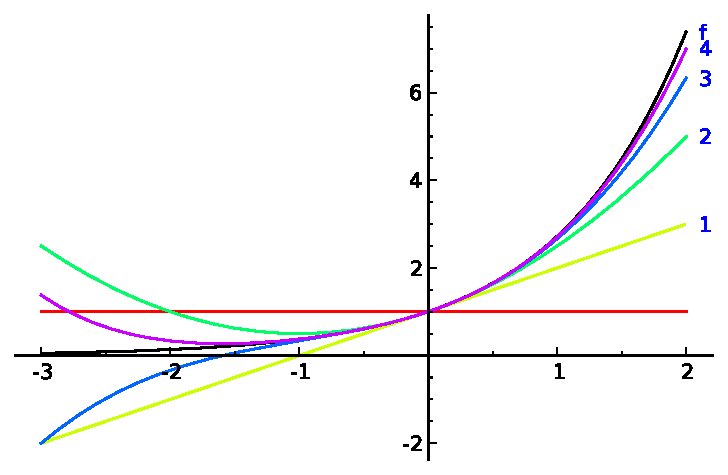
\includegraphics[width=\textwidth]{taylorexp.pdf}
 \end{center}

GEGEN

Die Funktion
\[ f(x) = \left \{ \begin{array}{ll}
\exp(-1/x^2), & \mbox{ für } x \neq 0\\
0, & \mbox{ für } x = 0\\
\end{array} \right. \]
ist nicht durch ihre Taylorreihe an $x_0=0$ darstellbar. Die Taylorreihe zu $f$
ist identisch $0$, da $f^{\,n}(0)=0$ ist für alle $n \in \mathbb{N}$. \\
\begin{sagein}
plot(exp(-1/x^2),(-0.5,0.5)) 
\end{sagein}
\begin{center}
  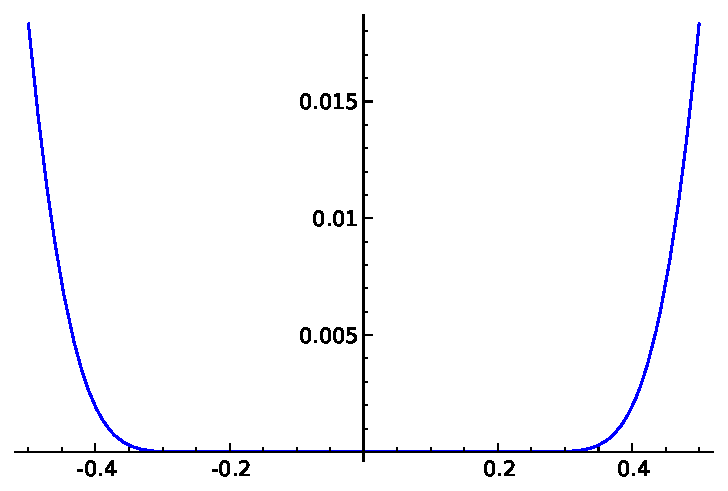
\includegraphics[height=4cm]{taylorgegen.pdf}
 \end{center}

inSAGE

\begin{sagein}
taylor(f, x, x0, n)
\end{sagein}
Taylorpolynom $(n-1)$-ten Grades zu einem Ausdruck $f$ 
(mit Unbekannten $x$) am Entwicklungspunkt $x0$. \\
\textbf{Beispiele}:
\begin{sagein}
taylor(1/(1-x),x,0,5)
\end{sagein}
{\color{blue}\[ x^{5} + x^{4} + x^{3} + x^{2} + x + 1\]}
\begin{sagein}
taylor(sin(x),x,2,5)
\end{sagein}
{\small\color{blue}\[ \frac{1}{24} \, {\left(x - 2\right)}^{4} \sin\left(2\right) -
\frac{1}{6} \, {\left(x - 2\right)}^{3} \cos\left(2\right) - \frac{1}{2}
\, {\left(x - 2\right)}^{2} \sin\left(2\right) + {\left(x - 2\right)}
\cos\left(2\right) + \sin\left(2\right)\]}

%%%%%%%%%%%%%%%%%%%%%%%%%%%%%%%%%%%%%%
\section{Integration}
%%%%%%%%%%%%%%%%%%%%%%%%%%%%%%%%%%%%%%

BEGRIFFE


  Sei $[a,b]$ ein Intervall. Gilt $a=a_0 < a_1 <a_2 < \dots <
                                 a_n=b$, so nennt man $Z=(a_0, \dots
                                 ,a_n)$ eine {\color{red} Zerlegung} von
                                 $[a,b]$.
 Eine Funktion $\phi:[a,b] \rightarrow \mathbb{R}$ heißt {\color{red}
                                 Treppenfunktion}, wenn es eine
                                 Zerlegung $Z$ von $[a,b]$ gibt, so dass
                                 $\phi$ konstant ist auf jedem
                                 Teilintervall $(a_i,a_{i+1})$ von $Z$.
 Wir erklären das Integral einer Treppenfunktion $\phi$ durch
\[\int_Z \phi := \sum_{k=1}^n c_k (a_k -a_{k-1}).\]
Dabei ist $Z$ die zugehörige Zerlegung und $c_k=\phi(x)$, $x\in
(a_{k-1},a_k)$.  
 Die Menge aller Treppenfunktionen auf $[a,b]$ sei $T[a,b]$.


Für eine beschränkte Funktion $f[a,b]\rightarrow \mathbb{R}$
heißt
\[ \int^*f:= \inf  \{ \int \psi \ | \ \psi \in T[a,b], f \leq \psi \}. \]
das {\color{red} Oberintegral} und 
\[ \int_*f:= \sup  \{ \int \psi \ | \ \psi \in T[a,b], f \geq \psi \}.\]
das {\color{red} Unterintegral}. Es gilt für $\phi, \psi \in T[a,b]$ mit
$\phi \leq f \leq \psi$ die Ungleichung
\[ \int \phi \leq \int_* f \leq \int^* f \leq \int \psi.\]

VIS

\begin{sagein}
f = Piecewise([[(-pi,0),(cos(x)).function(x)]])
rsf = f.riemann_sum(10,mode="midpoint")
P = f.plot(rgbcolor=(0.7,0.1,0.5), plot_points=40)
Q = rsf.plot(rgbcolor=(0.7,0.6,0.6), plot_points=40)
L = add([line([[b,0],[b,f(x=b)]],rgbcolor=(0.7,0.6,0.6))+line([[a,0],[a,f(x=a)]],rgbcolor=(0.7,0.6,0.6)) for (a,b),f in rsf.list()])
(P + Q +L)
\end{sagein}
\begin{center}
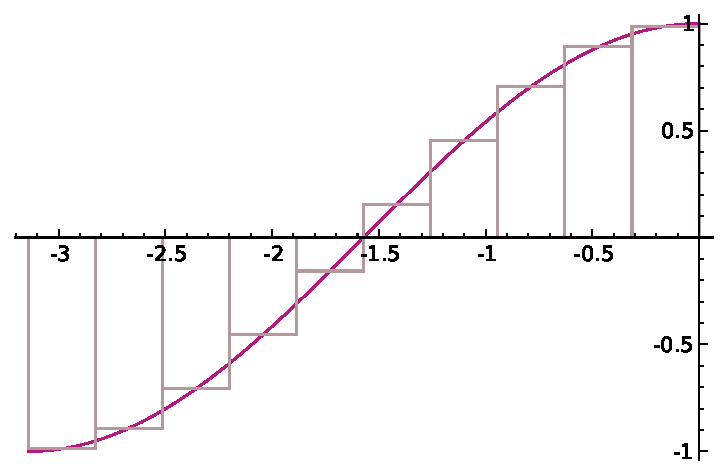
\includegraphics[width=6cm]{riemann.pdf}
\end{center}

RIE

Eine beschränkte Funktion $f:[a,b] \rightarrow \mathbb{R}$ heißt {\color{red}
integrierbar}, wenn Ober- und Unterintegral von $f$ auf $[a,b]$ übereinstimmen.\\
Der gemeinsame Wert heißt das {\color{red} Integral} von $f$ und wird mit 
\[ \int_a^b f(x)dx \]
bezeichnet.\\ 
($f$ der Integrand, $x$ Integrationsvariable, $a$, $b$ Integrationsgrenzen).

EIG


 Linearität
\[ \int_a^b (\alpha f + \beta g) dx = \alpha \int_a^b fdx + \beta
\int_a^b g dx \]
 Monotonie
\[  f \leq g \quad \Rightarrow \quad \int_a^b f dx \leq \int_a^b g
dx.\]
 Ist $f,g$ integrierbar, so auch $f+g$, $f*g$, $f-g$,
$\max\{f,g\}$, $\min \{f,g \}$. 


SÄTZE


 {\color{red} Stammfunktion} $F$: Ist $f$ stetig auf einem Intervall $I$ und $a \in I$, so ist 
\[F(x)= \int_a^x f(t) dt, x \in I \] eine differenzierbare Funktion mit
$F\,'(x)=f(x)$. 
 \emph{Unbestimmtes Integral}: alternative Notation für eine Stammfunktion $F$:  $\int f(x) dx$ 
 Ist $f$ stetig auf $[a,b]$, so gibt es ein $\xi \in [a,b]$ mit
\[\int_a^b f(x)dx = f(\xi) (b-a)\]


inSAGE


  Bestimmte Integrale der Form $\int_a^b f(x) dx$
\begin{sagein}
integrate(f,x,a,b) 
\end{sagein}
Dabei ist \isage{f} ein Ausdruck.
 Unbestimmte Integrale:
\begin{sagein}
integrate(f,x)
\end{sagein}
 Numerische Approximationen:
\begin{sagein}
numerical_integral(f,a,b) 
\end{sagein}
(benutzt die GSL-library).


BSP

\begin{sagein}
 integrate(sin(x),x,0,6)
\end{sagein}
\begin{sage}
-cos(6) + 1
\end{sage}
\begin{sagein}
integrate(exp(x)*x,x,2,3),integrate(exp(x)*x,x)
\end{sagein}
{\color{blue}\[\left(-e^{2} + 2 \, e^{3}, {\left(x - 1\right)} e^{x}\right)\]}
% \begin{sage}
% -e^2 + 2*e^3
% \end{sage}
\begin{sagein}
integrate(1/x^2,x,1,oo)
\end{sagein}
\begin{sage}
  1
\end{sage}
\begin{sagein}
numerical_integral(sin(1/x)*x,1,2)
\end{sagein}
\begin{sage}
  (0.91905916759870254, 1.0203606488609102e-14)
\end{sage}
\begin{sagein}
assume(a<>-1)
integrate(x^a*b,x)
\end{sagein}
{\color{blue} \[ \frac{b x^{{\left(a + 1\right)}}}{a + 1}\]}
% \begin{sage}
% b*x^(a + 1)/(a + 1)
% \end{sage}
\begin{sagein}
forget();a=-1
integrate(x^a*b,x)
\end{sagein}
{\color{blue} \[ b \log\left(x\right)\]}
% \begin{sage}
%  b*log(x)
% \end{sage}

UNEIG INT

Sei $f$ auf $[a,b)$ erklärt (eventuell $b=\infty$) und sei $f$ auf jedem
abgeschlossenen Teilintervall integrierbar. Man definiert
\[  \int_a^b f(x)dx := \lim_{z \rightarrow b (-0)} \int_a^z f(x)dx,\]
falls der Limes existiert. Man spricht von einem {\color{red}
uneigentlichen Integral}.

FKT FOLG


 Sei $(f_n)_n$ eine Folge integrierbarer Funktionen auf
$[a,b]$. Konvergiert $(f_n)_n$ gleichmäßig, so ist die Grenzfunktion
integrierbar mit
\[ \int_a^b \lim_{n \rightarrow \infty} f_n(x) dx = \lim_{n
\rightarrow \infty} \int_a^b f_n(x) dx .\]
 Sei $(f_n)_n$ eine Folge differenzierbarer Funktionen auf
$[a,b]$. $(f\,'_n)_n$ konvergiere gleichmäßig und es existiere ein $x_0
\in [a,b]$ für den $f_n(x_0)$ konvergiert. Dann konvergiert $(f_n)_n$
gleichmäßig mit $( \lim_{n \rightarrow \infty} f_n(x))' = \lim_{n
\rightarrow \infty} f\,'_n(x)$.  


%%%%%%%%%%%%%%%%%%%%%%%%%%%%%%%%%%%%%%
\chapter{bessereUeberschriftenFinden...}
\section{Umgang mit Strings}
%%%%%%%%%%%%%%%%%%%%%%%%%%%%%%%%%%%%%%

STRINGS


 Zeichenketten (engl. {\color{red} strings}) sind eine geordnete
Aneinanderreihung von Zeichen. Zeichen sind z.B. Buchstaben, Ziffern,
Sonderzeichen,...
 Mit ihnen kann man in Sage Texte gestalten. Sie sind wichtig
für die Ausgabe der Ergebnisse.
 Datentyp \isage{str}.
 eingeschlossen in Hochkommas oder Anführungszeichen.


BSP

\begin{sagein}
text1 = 'Dies ist ein String.'; text1
\end{sagein}
\begin{sage}
'Dies ist ein String.'
\end{sage}
\begin{sagein}
text2 = "Dies ist noch ein String."; text2
\end{sagein}
\begin{sage}
'Dies ist noch ein String.'
\end{sage}
\begin{sagein}
type(text1)
\end{sagein}
\begin{sage}
<type 'str'>
\end{sage}figures/

ZUGRIFF


 Indexoperator {\color{blue}$[\ ]$}:
\begin{sagein}
text1[0], text1[3], text1[2:4], text1[0:4:2]
\end{sagein}
\begin{sage}
('D', 's', 'es', 'De')
\end{sage}
 Ersetzungen innerhalb des Strings:
\begin{sagein}
text1.replace('Dies','Das')
\end{sagein}
\begin{sage}
'Das ist ein String.'
\end{sage}


OPERATIONEN


 Zusammenhängen von Strings
\begin{sagein}
A='Letzte '; B='Vorlesung'; A+B
\end{sagein}
\begin{sage}
'Letzte Vorlesung'
\end{sage}
 \isage{len()} gibt die Anzahl der Zeichen in einer Zeichenkette
an.
\begin{sagein}
a=len(A+B); a
\end{sagein}
\begin{sage}
  16
\end{sage}
  Zugriffe beginnend vom Ende
\begin{sagein}
(A+B)[-1]
\end{sagein}
\begin{sage}
  'g'
\end{sage}
 {\color{blue} \isage{str()}} wandelt Objekte in einen String um.
\begin{sagein}
str(x^2+2), str([1,2,3])
\end{sagein}
\begin{sage}
('x^2 + 2', '[1, 2, 3]')
\end{sage}
 \isage{find()}: Strings durchsuchen
\begin{sagein}
'Hallo'.find('lo')
\end{sagein}
\begin{sage}
3
\end{sage}
 
\begin{sagein}
'Hallo'.find('gnu')
\end{sagein}
\begin{sage}
-1
\end{sage}
 \isage{split()}: Aufspalten von Texten
\begin{sagein}
text = 'Dies ist ein Satz, und ein Nebensatz'
text.split() 
\end{sagein}
\begin{sage}
 ['Dies', 'ist', 'ein', 'Satz,', 'und', 'ein', 'Nebensatz']
\end{sage}
\begin{sagein}
text.split('i')
\end{sagein}
\begin{sage}
['D', 'es ', 'st e', 'n Satz, und e', 'n Nebensatz']
\end{sage}


print/Formate

\begin{sagein}
  print 'Text %<format> und %<format> ... ' % (x,y,...)
 \end{sagein}
\isage{<format>}:
\begin{sagein}
%[<flag>][<minwidth>][.<precision>]converter 
\end{sagein}

 \isage{flag}: 0 für das Auffüllen mit Nullen
 \isage{minwidth}: Minimale Breite der Darstellung
 \isage{precision}: Genauigkeit (Nachkommastellen)
 \isage{converter}:
\begin{tabular}{cp{10cm}}
\isage{'i'} & ganze Zahl mit Vorzeichen\\
\isage{'e'} & Gleitkommazahl mit exponentialformat (kleingeschrieben).\\
\isage{'f'} &Gleitkommazahl im Dezimalformat.\\
\isage{'g'} &Gleitkommazahl. Benutzt kleingeschriebene Exponentialform wenn der Exponent kleiner als -4 oder der Genauigkeit ist, ansonsten Dezimalformat.
\end{tabular}


BSP

\begin{sagein}
print '%5s | %7s' % ('Index','Wert')
for k in srange(1,25,9.55): 
    print '%5i | %07.3f' % (k,k^2) 
\end{sagein}
\begin{sage}
Index |    Wert
    1 | 001.000
   10 | 111.303
   20 | 404.010
\end{sage}
figures/
interact

\begin{sagein}
@interact
def _(b = range_slider(-20, 20, 1, default=(-19,3), label='Range')):
    plot(sin(x)/x, b[0], b[1]).show(xmin=b[0],xmax=b[1]) 
\end{sagein}
\begin{center}
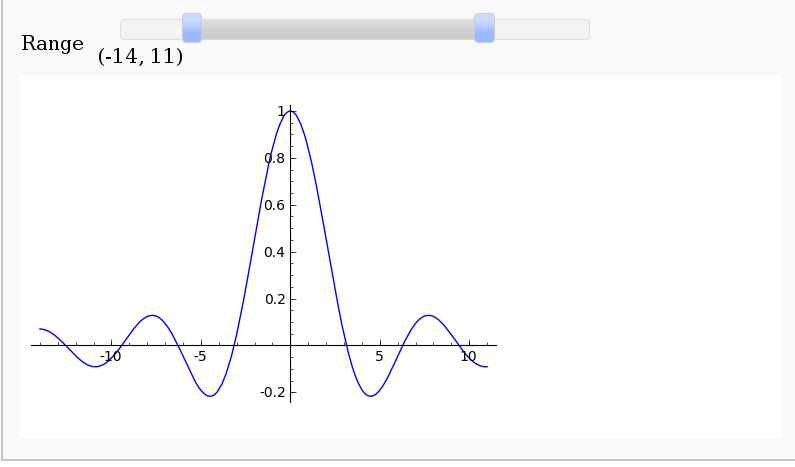
\includegraphics[width=0.8\textwidth]{interact_basis.png}
\end{center}


 Regler mit Werten von vmin bis vmax
\begin{sagein}
u=slider(vmin, vmax=, step_size=1, default=, label=) 
\end{sagein}
 Regler eines Intervalles
\begin{sagein}
u=range_slider(vmin, vmax=, step_size=1, default=, label=)
\end{sagein}
 Eine Ankreuzfeld
\begin{sagein}
u=checkbox(default=True, label=)
\end{sagein}
 Ein Aufklappmenü oder Knöpfe (Knöpfe wenn nrows, ncols, oder buttons gesetzt ist, sonst Aufklappmenü)
\begin{sagein}
u=selector(values, label=, nrows=, ncols=, buttons=False)
\end{sagein}
 Ein Textblock
\begin{sagein}
u=text_control(value='')
\end{sagein}



TAYLOR

\begin{center}
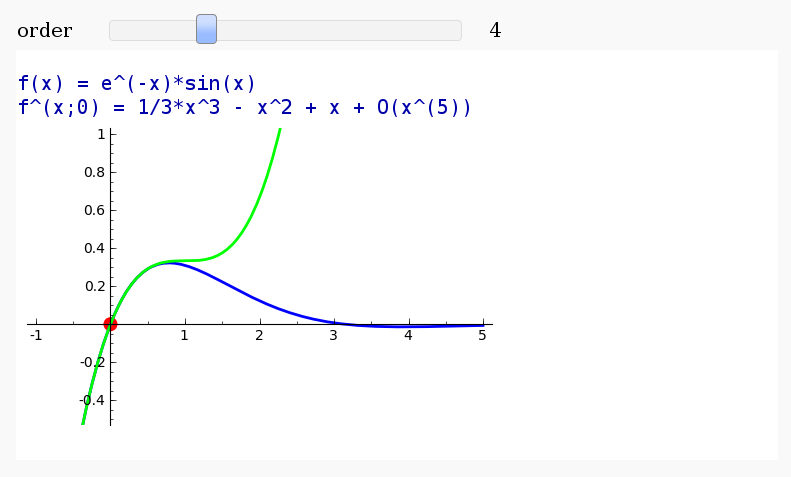
\includegraphics[width=\textwidth]{interact1.png}
\end{center}

\begin{sagein}
var('x')
x0  = 0
f   = sin(x)*e^(-x)
p   = plot(f,-1,5, thickness=2)
dot = point((x0,f(x=x0)),pointsize=80,rgbcolor=(1,0,0))
@interact
def tayl(order=slider(1,12,1,label='order')):
    ft = f.taylor(x,x0,order)
    pt = plot(ft,-1, 5, color='green', thickness=2)
    print ('f(x) = %s'% f)
    print ('f^(x;%s) = %s + O(x^(%s))'%(x0,ft,order+1))
    show(dot + p + pt, ymin = -.5, ymax = 1)
\end{sagein}

ABSTAND

\begin{center}
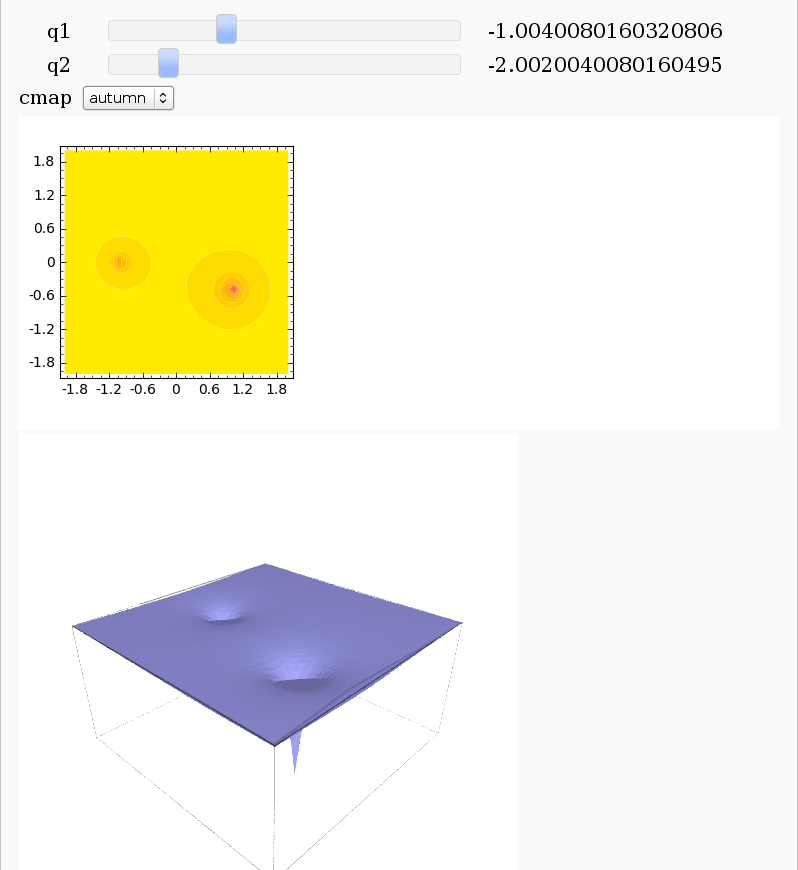
\includegraphics[width=7.5cm]{interact2.png}
\end{center}

\begin{sagein}
@interact
def _(q1=slider(-3,3,default=-1), q2=slider(-3,3,default=-2), cmap=selector(['autumn', 'bone', 'cool', 'copper', 'gray', 'hot', 'hsv','jet', 'pink', 'prism', 'spring', 'summer','winter'])):
     x,y = var('x,y')
     f = q1/sqrt((x+1)^2 + y^2) + q2/sqrt((x-1)^2+(y+0.5)^2)
     C = contour_plot(f, (x,-2,2), (y,-2,2), plot_points=30, contours=15, cmap=cmap)
     show(C, figsize=3, aspect_ratio=1)
     show(plot3d(f, (x,-2,2), (y,-2,2)), figsize=5, viewer='tachyon')
\end{sagein}

GeoGebra


  In GeoGebra: Erstellen eines Objektes
 In GeoGebra: File> Export> Dynamic worksheet.
 In Sage notebook: Data> Die .jar (von GeoGebra) und die .ggb hochladen.
 Aus dem Exportierten .html den Teil mit <applet> kopieren und im worksheet in Sage unter Edit kopieren( Edit> Paste ).
 Im Editier-tab die codebase zu "./data/" ändern
 Fertig!


\begin{center}
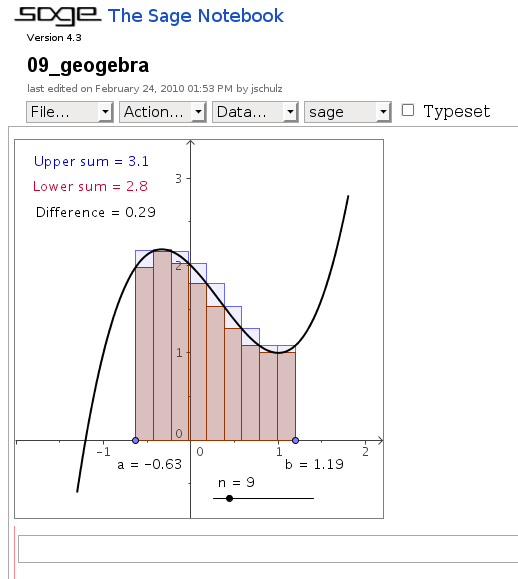
\includegraphics[width=0.6\textwidth]{geogebra.png}
\end{center}

%%%%%%%%%%%%%%%%%%%%%%%%%%%%%%%%%%%%%%
\section{Vertiefung Programmierung}
%%%%%%%%%%%%%%%%%%%%%%%%%%%%%%%%%%%%%%

GGT

Berechnung des ggT von natürlichen Zahlen $a$ und $b$ mit Hilfe des
euklidischen Algorithmus.
\bigskip

\textbf{Idee:} Es gilt:

  $ggT(a,b)=ggT(a,b-a)$ für $a<b$.
 $ggT(a,b)=ggT(b,a)$.
 $ggT(a,a)=a$.


\textbf{Algorithmus:}

Wiederhole,  bis $a=b$
 
 Ist $a>b$, so $a=a-b$.
 Ist $a<b$, so $b=b-a$ 


\begin{sagein}
def ggT(a,b):  
    """Bestimme den ggT von a und b"""
    while a<>b:
        if a>b:
            a = a-b
        else: 
            b = b-a
    return a
ggT(6,9)
\end{sagein}
\begin{sage}
3  
\end{sage}

PRIM TWIN

\begin{sagein}
T = []; anz = 0
for i in [2..100]:
    if (is_prime(i) and is_prime(i+2)):
        anz += 1
        T.append([i,i+2])
print('Anzahl = %s' % anz);T
\end{sagein}
\begin{sage}
Anzahl = 8
[[3, 5], [5, 7], [11, 13], [17, 19], [29, 31], [41, 43], [59, 61], [71,
73]]
\end{sage}

ABS

\begin{sagein}
def betrag(a):
    if a in ZZ or a in QQ or a in RR:
        if a>0:
            y = a
        else:
            y = -a
    elif a in CC:
        y = sqrt(real(a)^2+imag(a)^2)
    else:
        return 'Falscher Eingabetyp'
    return y
betrag([1,2]), betrag(2+I*2)
\end{sagein}
\begin{sage}
('Falscher Eingabetyp', 2*sqrt(2))
\end{sage}

GÜLT VAR


 Mit der Gültigkeit von Variablen ist die Bestandsdauer von
   Variablen bzw. der Werten dieser Variablen gemeint.
 \emph{globale Variablen}: Im aktuellen Worksheet sind alle Variablen/Funktionen global, 
d.h. die den Variablen zugewiesenen Werte bleiben für die
gesamte Laufzeit vom jeweiligen worksheet erhalten bis sie geändert werden. 
Man kann auf die Variablen jederzeit zugreifen und die Werte der Variablen
ändern.
 \emph{lokale Variablen}: Diese sind nur innerhalb einer Prozedur/Funktion 
gültig. Nach Beenden der Prozedur werden
diese Variablen wieder gelöscht. 


MANDELBROT

Die Mandelbrot-Menge ist die Menge von Punkten $c \in \mathbb{C}$
bei denen die Folge $(z_n)_n$, die durch
\[ z_0:=c, \qquad  z_{n+1} = z_n^2 +c, \quad n \in \mathbb{N}\]
definiert ist, beschränkt ist.

\begin{sagein}
def mandel(x,y):
    c = (x + I*y).n()
    z = c
    it = 0
    max_it = 150
    while abs(z)<2 and it<max_it:
        z = z^2 + c
        it += 1
    return float(it/max_it)
\end{sagein}
Die Funktion \isage{mandel} gibt zu $x+iy$ die relative Anzahl der
Iterationsschritte zurück.

\begin{sagein}
density_plot(mandel, (-2.1,1.2), (-1.1,1.1), plot_points=100)
\end{sagein}
\begin{center}
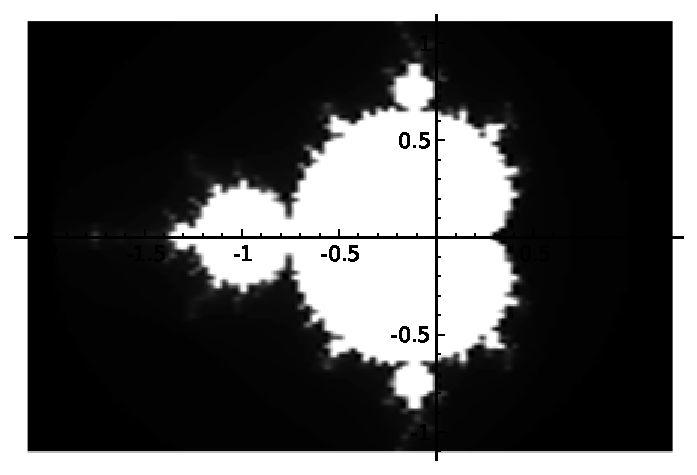
\includegraphics[width=0.8\textwidth]{mandel.pdf} 
\end{center}

PROG REGELN


 \emph{Hilfetext}: Ein Programm sollte im Hilfetext eine gute Beschreibung der Funktionsweise der Funktion enthalten. Dieser sollte insbesondere Ein- und Ausgabe-Variablen genau beschreiben.
 \emph{Kommentieren}: Im Programm sollte durch Kommentare dokumentiert werden, was einzelne, wesentliche Abschnitte/Zeilen im Programm tun.
 \emph{Passende Benennung von Variablen/Funktionen}: Variablen und Funktionen sollten durchdacht benannt werden, d.h. man sollte an ihnen im Optimum direkt erkennen können, welchem Zweck sie im gegebenen Kontext dienen. 


LAST BSP

\begin{sagein}
def Gadisch(x,basis):
    """Berechnung der Darstellung einer natuerlichen Zahl 
x zur Basis b. Rueckgabe des Ergebnis als Liste!"""
    #Abfangen der Eingabe
    if not x in ZZ or x < 0 or basis==1: 
        return 'Eingabe nicht korrekt!'
    T = []  # leere Liste 
    while x>0:
        T.append(x%basis) # Rest der Division
        print '%i : %i = %i Rest %i' % (x,basis,floor(x/basis),x%basis)
        x = floor(x/basis) # Teiler setzen
    # Rueckgabe der Liste
    return T
\end{sagein}

\begin{sagein}
Gadisch(6,2)
\end{sagein}
\begin{sage}
6 : 2 = 3 Rest 0
3 : 2 = 1 Rest 1
1 : 2 = 0 Rest 1
[0, 1, 1]
\end{sage}

\begin{sagein}
Gadisch(3.4,2)
\end{sagein}
\begin{sage}
'Eingabe nicht korrekt!'
\end{sage}

ALLERLAST BSP xD
KOCH


 Seien $y_1,y_2$ zwei Punkte im $\mathbb{R}^2$. 
 Betrachte die Strecke mit Endpunkten $y_1$ und $y_2$.  
 Ersetze  diese Strecke durch 4 Strecken 
$\overline{y_1 z_1}$, $\overline{z_1 z_2}$, $\overline{z_2 z_3}$,
$\overline{z_3 y_2}$ mit Endpunkten 
\begin{eqnarray*}
 z_1 &=&\frac23 y_1 + \frac13 y_2\\[0.5cm]
 z_2 &=& \frac{\sqrt{3}}{6} \left( \begin{array}{cc}
 0 & 1 \\ -1 & 0 \\
 \end{array} \right)
 (y_1 - y_2) + \frac12 (y_1 + y_2)\\[0.5cm]
 z_3 &=&\frac13 y_1 + \frac23 y_2
\end{eqnarray*}
 Dieses Prozedere wird nun für jede einzelne Teilstrecke wiederholt.


\begin{sagein}
def koch(y1,y2,lev):
    Listelinien = []
    if (lev == 0):
        Listelinien.append(line([(y1[0],y1[1]),(y2[0],y2[1])]))
    else:
        # Definieren der neuen Punkte 
        z1 = 2/3 * y1 + 1/3 * y2
        z3 = 1/3 * y1 + 2/3 * y2
        z2 = sqrt(3)/6*matrix([[0, 1],[ -1, 0]])*(y1-y2) + 1/2 * (y1 + y2)
        # Definieren der 4 Strecken
        Listelinien.append(koch(y1, z1, lev-1))
        Listelinien.append(koch(z1, z2, lev-1))
        Listelinien.append(koch(z2, z3, lev-1))
        Listelinien.append(koch(z3, y2, lev-1))
    return add(Listelinien)
\end{sagein}

\begin{sagein}
# Einfacher Fall einer Linie 
koch(vector([0,0]),vector([1,0]),4)
\end{sagein}
\begin{center}
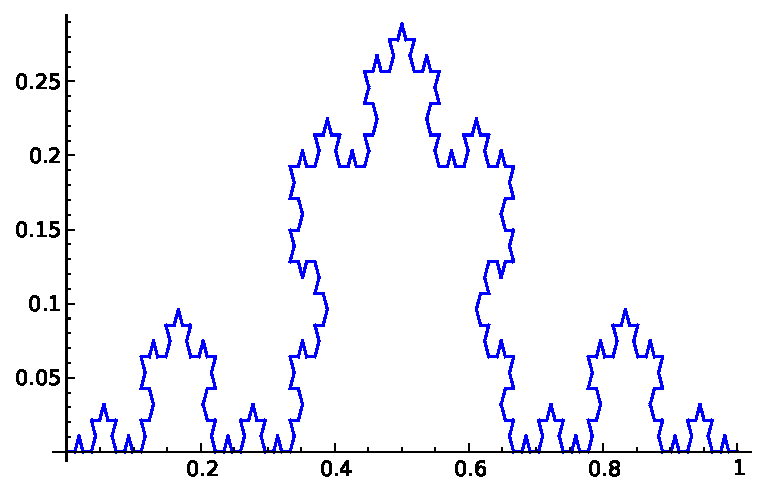
\includegraphics[width=0.7\textwidth]{koch.pdf} 
\end{center}


\end{document}